\documentclass[twocolumn,amsmath,amssymb,pra]{revtex4-2}
\usepackage[utf8]{inputenc}
\usepackage{amsmath}
\usepackage{graphicx}
\graphicspath{ {figures/} }
\usepackage{siunitx}
\usepackage{hyperref}
\usepackage{float}
\usepackage{lipsum}


\begin{document}

\title{Fourier Optics}

\author{Raymond Fang, Jun Sung}

\date{11/11/21}
\begin{abstract}
Abstract: A 4-f apparatus was aligned for the purpose of testing the Fourier transforming properties of a simple optical system. A camera was used to photograph an image of an object, an image at the Fourier plane of the system, and an image at the image plane. We found that the image at the Fourier plane was the Fourier Transform of the object. Great qualitative and quantitative agreement between the image at the Fourier plane and theoretical Fourier Transform was observed. The image at the image plane reconstructed the original image, indicating that the second lens of the 4-f apparatus acted as an inverse Fourier transform. Additionally an aperture was placed at the Fourier plane. We found that placement of an aperture at the Fourier plane acted as a low-pass filter, with smaller aperture sizes corresponding to more blurry features.
      
\end{abstract}
\maketitle

\section{Introduction}
Fourier transforms are a foundational aspect of optics when it comes to describing light propagation. In particular, we have that lenses can be used to generate the Fourier transform of optical fields from a source if one looks at the appropriate plane, which we will refer to as the Fourier plane. This gives us the opportunity to filter optical fields in the Fourier space. In this lab, we shall look at the Fourier transform of various filters, which will allow for us to gain a firm understanding on how lenses transform the optical information emitted by such filters.

\subsection{A Brief Overview of Methods}
This lab consists of two main parts:
\begin{itemize}
    \item Observing the Fourier and inverse Fourier transforms of various filters
    \item Observing how a low-pass filter affects the Fourier transform
\end{itemize}
For the first part, we position the camera in the Fourier and image plane (depicted in Figure \ref{fig:app}) which allows for us to take pictures of the resulting Fourier and inverse Fourier transforms of various filters. We will then compare the captured Fourier transforms with the expected/calculated Fourier transforms (done through Mathematica) for each of the filters.

For the second part, we place a pinhole/variable aperture at the Fourier plane, which will act as a low-pass filter for our Fourier transform. We then place a camera in the image plane, which allows for us to view the resulting inverse Fourier transform. Using Mathematica, we now calculate the Fourier transform of our capture inverse Fourier transform; this allows for us to see the effects of the pinhole/variable aperture on the Fourier transform.

\subsection{Applications}

First and foremost,the principles in Fourier optics are useful in the design of optical systems. For example, one often wants to reduce aberrations in the output of lasers to produce the highest quality data for experiments. Modifications to the shape of the beam at the focal plane can be related to the beam profile at different points in space. As an example, the beam often has an airy disk profile at the focal plane. An aperture can thus be placed at the focal plane to produce a beam with a more smooth intensity profile. In this lab, we shall demonstrate some of the effects of adding a pinhole at the focal plane.

Aside from better understanding optical systems, the principles of Fourier optics also have industrial applications. One interesting example is that of computer-generated holography, where it is desired to generate holographic images of objects in the real world. Initial attempts at this were done from wave front calculations but this proved to be very difficult to do computationally. Computing the Fourier transform is much faster and is often used for computer-generated holography. In this case, the Fourier transform is used to determine what light pattern needs to be inputted into a series of lens to generate a desired image at the holograph plane. Although these calculations initially only worked in two dimensions, researchers have begun to show that three dimensional reconstructions are possible \cite{brown1969computer}! 

\section{Theory}

\subsection{Optical Fourier Transform Produced by a Lens}

To conceptualize how a lens produces the Fourier transform of an object at its focal place, consider incoming light from an object illuminating the lens. The incoming wave from the object can be written as a superposition of plane waves (mathematically this is equivalent to writing an equation as a sum of its basis elements, which are plane waves in this case). The key to understanding the image formed at the focal plane is thus understanding where each component plane wave, which correspond to different spatial frequencies, is positioned at the focal plane\cite{tyson2014principles}. 

The equation for a plane wave is given by Eqn. \ref{Plane_wave}, where the angular wave number is given by Eqn. \ref{Wavevector}. For the purposes of our experiment, we shall assume the beam propagates along the z axis without loss of generality. Using the relation for spatial frequency $\upsilon_x = \frac{k_x}{2\pi}$ (all equations in the x plane can also be similarly written in the y plane), we can write the the plane wave at the initial lens, placed at $z = 0$, as Eqn. \ref{Spatial_Freq}. $\upsilon_x$ has units of cycles per unit distance.

\begin{equation}
    U(x,y,z) = Ae^{(i(k_xx+k_yy+kz_z))}
    \label{Plane_wave}    
\end{equation}

\begin{equation}
    k = (k_x^2+k_y^2+k_Z^2)^{1/2} = \frac{2\pi}{\lambda}
    \label{Wavevector}    
\end{equation}

\begin{equation}
    f(x,y) = Ae^{2i\pi(\upsilon_xx+\upsilon_yy)}
    \label{Spatial_Freq}
\end{equation}

Given that vector k makes an angle $\theta_x = sin^{-1}(\frac{k_x}{k})$ with the z axis (propagation axis), we can relate the spatial frequency with the angle of the wave from the z axis as Eqn. \ref{Spatial_Angle}.

\begin{equation}
    \theta_x = sin^{-1}\lambda\upsilon_x
    \label{Spatial_Angle}
\end{equation}

The paraxial approximation is the condition where the plane waves make small angles relative to the optical axis (which is the z-axis in our case). In other words, the beam travels approximately parallel to the optical axis. The conditions for the paraxial approximation to be true is $k_x<<k$ and $k_y<<k$, which is true for laser beams. Under the paraxial approximation $sin(\theta)\approx \theta$ and we can write the angle the wave makes from the z axis at the lens with Eqn. \ref{Paraxial_Spatial_Freq}. It is noted that the angle is linearly proportional to the spatial frequency along the axis \cite{tyson2014principles}.

\begin{equation}
    \theta_x \approx \lambda\upsilon_x
    \label{Paraxial_Spatial_Freq}
\end{equation}

The lens focus a plane wave propagating with angle ($\theta_x$,$\theta_y$) to the location ($\theta_xf$,$\theta_yf$) in the focal plane, where f is the focal length. Applying Eqn. \ref{Paraxial_Spatial_Freq}, we see that a wave with spatial frequency ($\upsilon_x$,$\upsilon_y$) is focused to position ($\upsilon_x\lambda f$,$\upsilon_y\lambda f$) at the focal plane. Thus the position of a plane wave in the x-y plane at the focal plane is linearly proportion to its spatial frequencies ($\upsilon_x$,$\upsilon_y$). In other words, the image viewed at the focal plane of the lens is simply the Fourier transform of the image \cite{tyson2014principles}. 

\subsection{Inverse Fourier Transform}
Next, we shall see how propagation of light away from the focal plane to the second focusing lens produces the inverse Fourier transform. From  a pure optics perspective, the 4-f apparatus used in the experiment ought to produce an image of the object. Thus it makes intuitive sense that if the light rays at the focal plane produce the Fourier transform, that the second lens must be applying the inverse Fourier transform to create an image of the object. 

Next, we will show mathematically how propagation of the wave from the focus plane produces the inverse Fourier transform. Suppose the focal plane has coordinates z = A and we want to observe the electric field at coordinates z = B = A + d. The electric field from a point source at plane z = A at position ($x_i$,$y_i$) is given by Eqn. \ref{Point Source}:

\begin{equation}
    E(x,y,B) \simeq \frac{1}{d}e^{ikd}e^{ik((x-x_i)^2+(y-y_i)^2)/2d}
    \label{Point Source}
\end{equation}

The electric field at plane z = B would simply be the the superposition of Eqn. \ref{Point Source} for all the point sources at the focal plane z = A, where each point source corresponds to a frequency in the Fourier plane. After dropping some constants and dropping quadratic terms in the integral (which is okay since the field at the focal plane lies close to the z axis or $kx_i^2/2d <<\pi$), the electric field at the far field or after a second lens reduces to Eqn.\ref{IFFT}. This is simply the inverse Fourier transform of the electric field at the focal plane z = A \cite{tyson2014principles}.

\begin{equation}
    E(x,y,B) \simeq \int_{-\infty}^{\infty}\int_{-\infty}^{\infty} E(x_i,y_i,A)e^{-i2\pi(xx_i+yy_i)/\lambda d}dx_idy_i
    \label{IFFT}
\end{equation}

\begin{figure*}[ht]
    \centering
    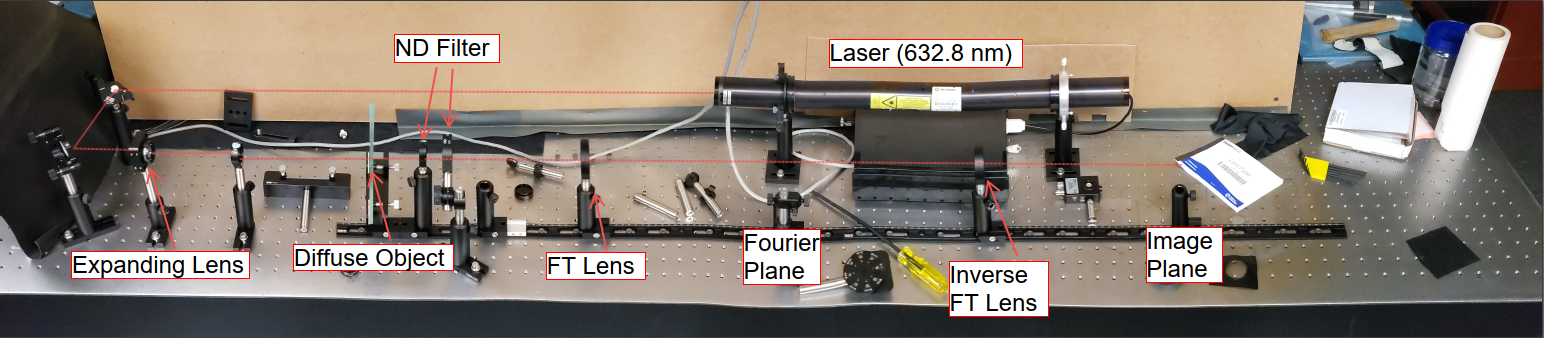
\includegraphics[ width =  \textwidth ]{apparatus.PNG}
    \caption{The apparatus used for this lab}
    \label{fig:app}
\end{figure*}

\section{Apparatus}

\subsection{Apparatus Design}
The design of our apparatus has the purpose of observing the Fourier transform of our diffuse object as well as the image formed after it passes through the inverse Fourier transform lens. A schematic diagram of the "4-$f$" Fourier transform apparatus we used can be seen in Figure \ref{fig:app_schem}, and a labelled photograph of our apparatus can be seen in Figure \ref{fig:app}.
\begin{figure}[H]
    \centering
    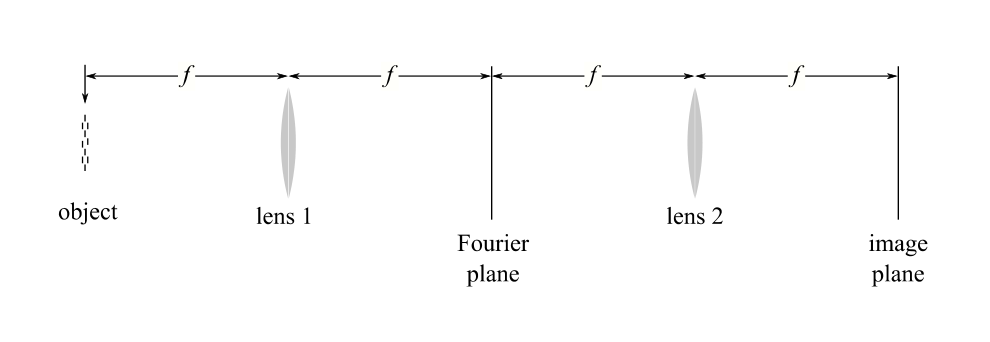
\includegraphics[ width = 0.9 \linewidth ]{schematic_apparatus.PNG}
    \caption{A schematic diagram of the "4-$f$" Fourier transform apparatus}
    \label{fig:app_schem}
\end{figure}
The laser that we used for this lab is the JDS Uniphase 1100 Series red helium-neon laser. In particular, the model number of our laser is 1145P-3494, and the wavelength of the laser is $632.8 \ \si{nm}$. More information on this laser can be found in the manual, location at \cite{laser}.
\begin{figure}[H]
    \centering
    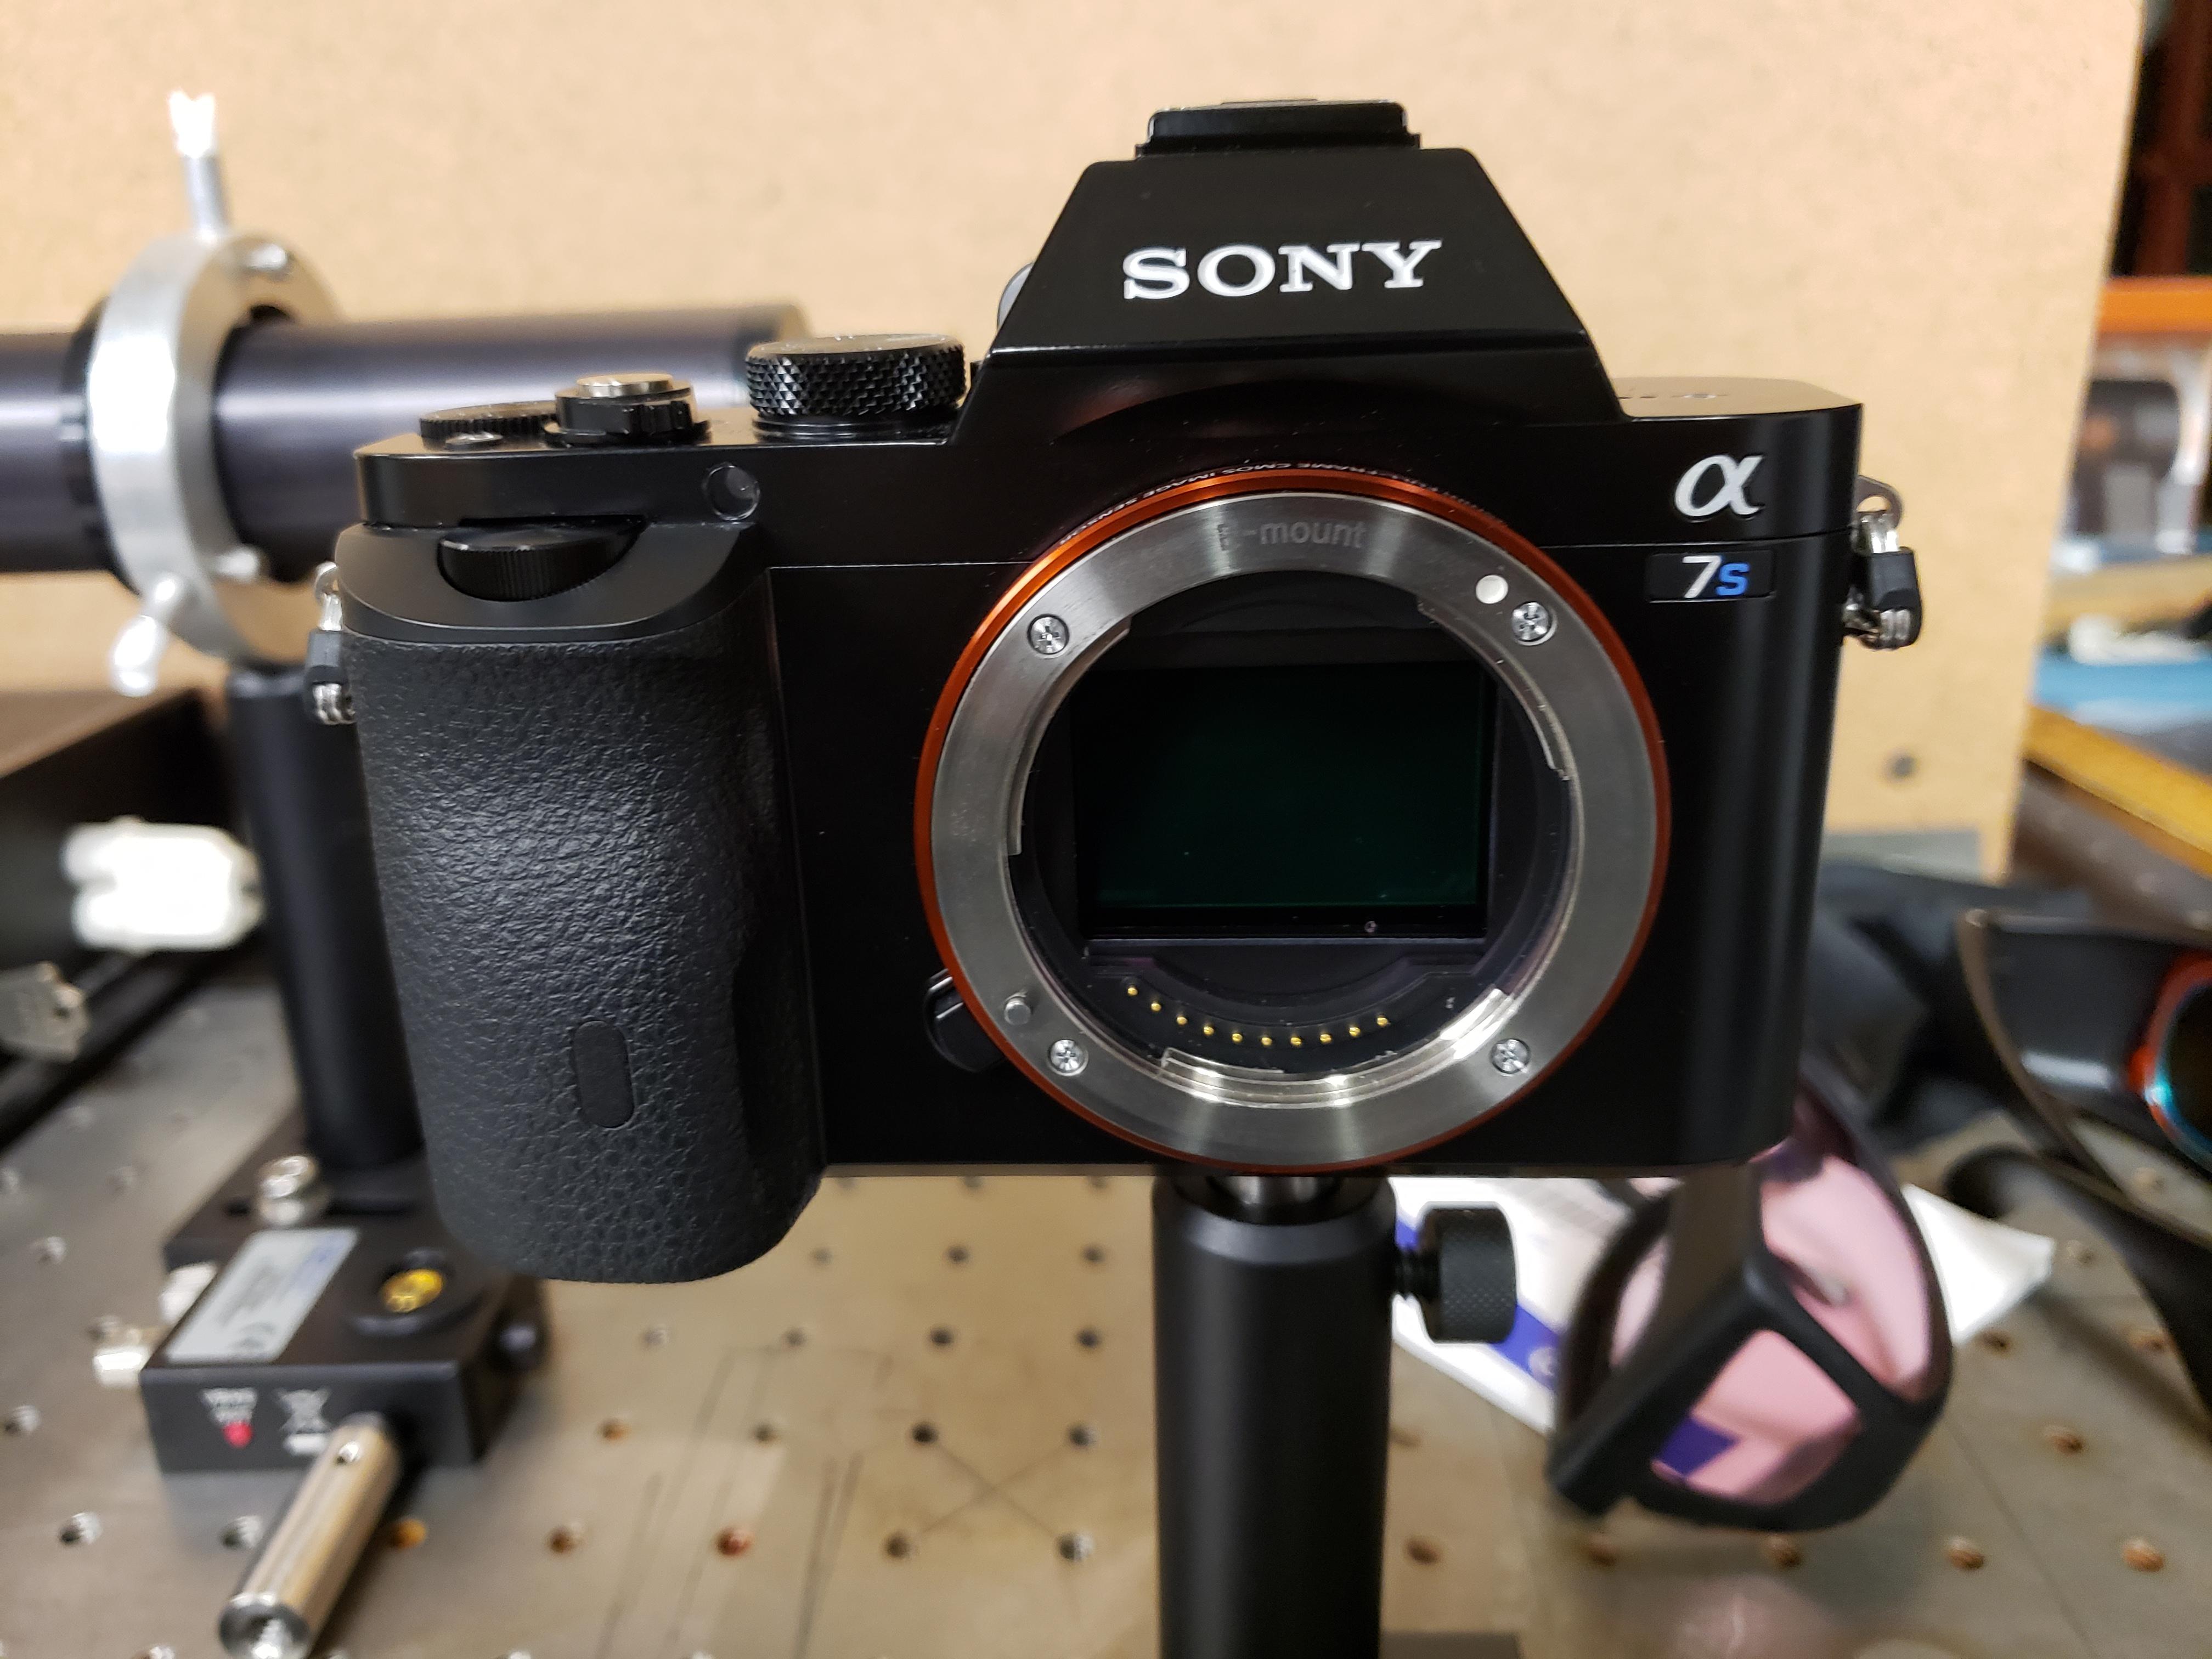
\includegraphics[ width = 0.9 \linewidth ]{camera.jpg}
    \caption{The camera that we used for this lab}
    \label{fig:camera}
\end{figure}
The camera that we used for this lab can be seen in Figure \ref{fig:camera}. The model of this Sony camera is ICLE-7S, and its main function in this lab was to take pictures of the laser at the Fourier and image plane (as shown in Figure \ref{fig:app}). More information on this camera (as well as the manual) can be found at \cite{camera}.

Before we observed the Fourier transform of various filters, we had to make sure that the laser was well-aligned; that is, we needed to make sure that the laser is propagating directly parallel to the axis where our lenses and camera are situated in. To align the laser, we first put two apertures (at their smallest opening) at the Fourier plane and image plane and then adjusted the mirrors left of the expanding lens until we saw the laser going through both of the aperture openings. 

Once the laser was aligned, we then had to make optimize the image that the camera was picking up. We started by collimating our laser by using the expanding lens as shown in Figure \ref{fig:app}. The reason for why we do so is because it magnifies the image that the camera will pick up -- making it easier for us to view the features of our resulting Fourier transform. Once collimated, we then made sure to reduce the intensity of the incoming laser by using two ND filters (as shown in Figure \ref{fig:app} as well), and adjusted the exposure of our camera so that it is at a minimum. By doing so, the image that we capture using the camera is not overly saturated, which results in the features of our resulting Fourier transform to show up more clearly and distinctly.

\subsection{Observing the Fourier Transform}
With the laser well-aligned and the image optimized, all that is left to do is to capture both the Fourier and inverse Fourier transform of various filters (that is configured where the diffuse object is located in Figure \ref{fig:app}). This is done by placing the camera at both the Fourier and image plane, respectively, and taking a picture of the laser. Figure \ref{fig:filters} shows the filters that we used to observe the Fourier and inverse Fourier transform. The resulting images can be seen in the Appendix.
\begin{figure}
    \centering
    \includegraphics[ width = 0.9\linewidth ]{filters.jpg}
    \caption{The filters that we used for this lab. For the rest of this lab, I shall refer to these filters as "filter \#", where the number starts at 1 and increases from left to right, top to bottom.}
    \label{fig:filters}
\end{figure}

\subsection{Observing How a Low-Pass Filter Affects the Fourier Transform}
For this part of the lab, we used a pinhole/variable aperture (as shown in Figure \ref{fig:aperture}) to act as our low-pass filter. 
\begin{figure}
    \centering
    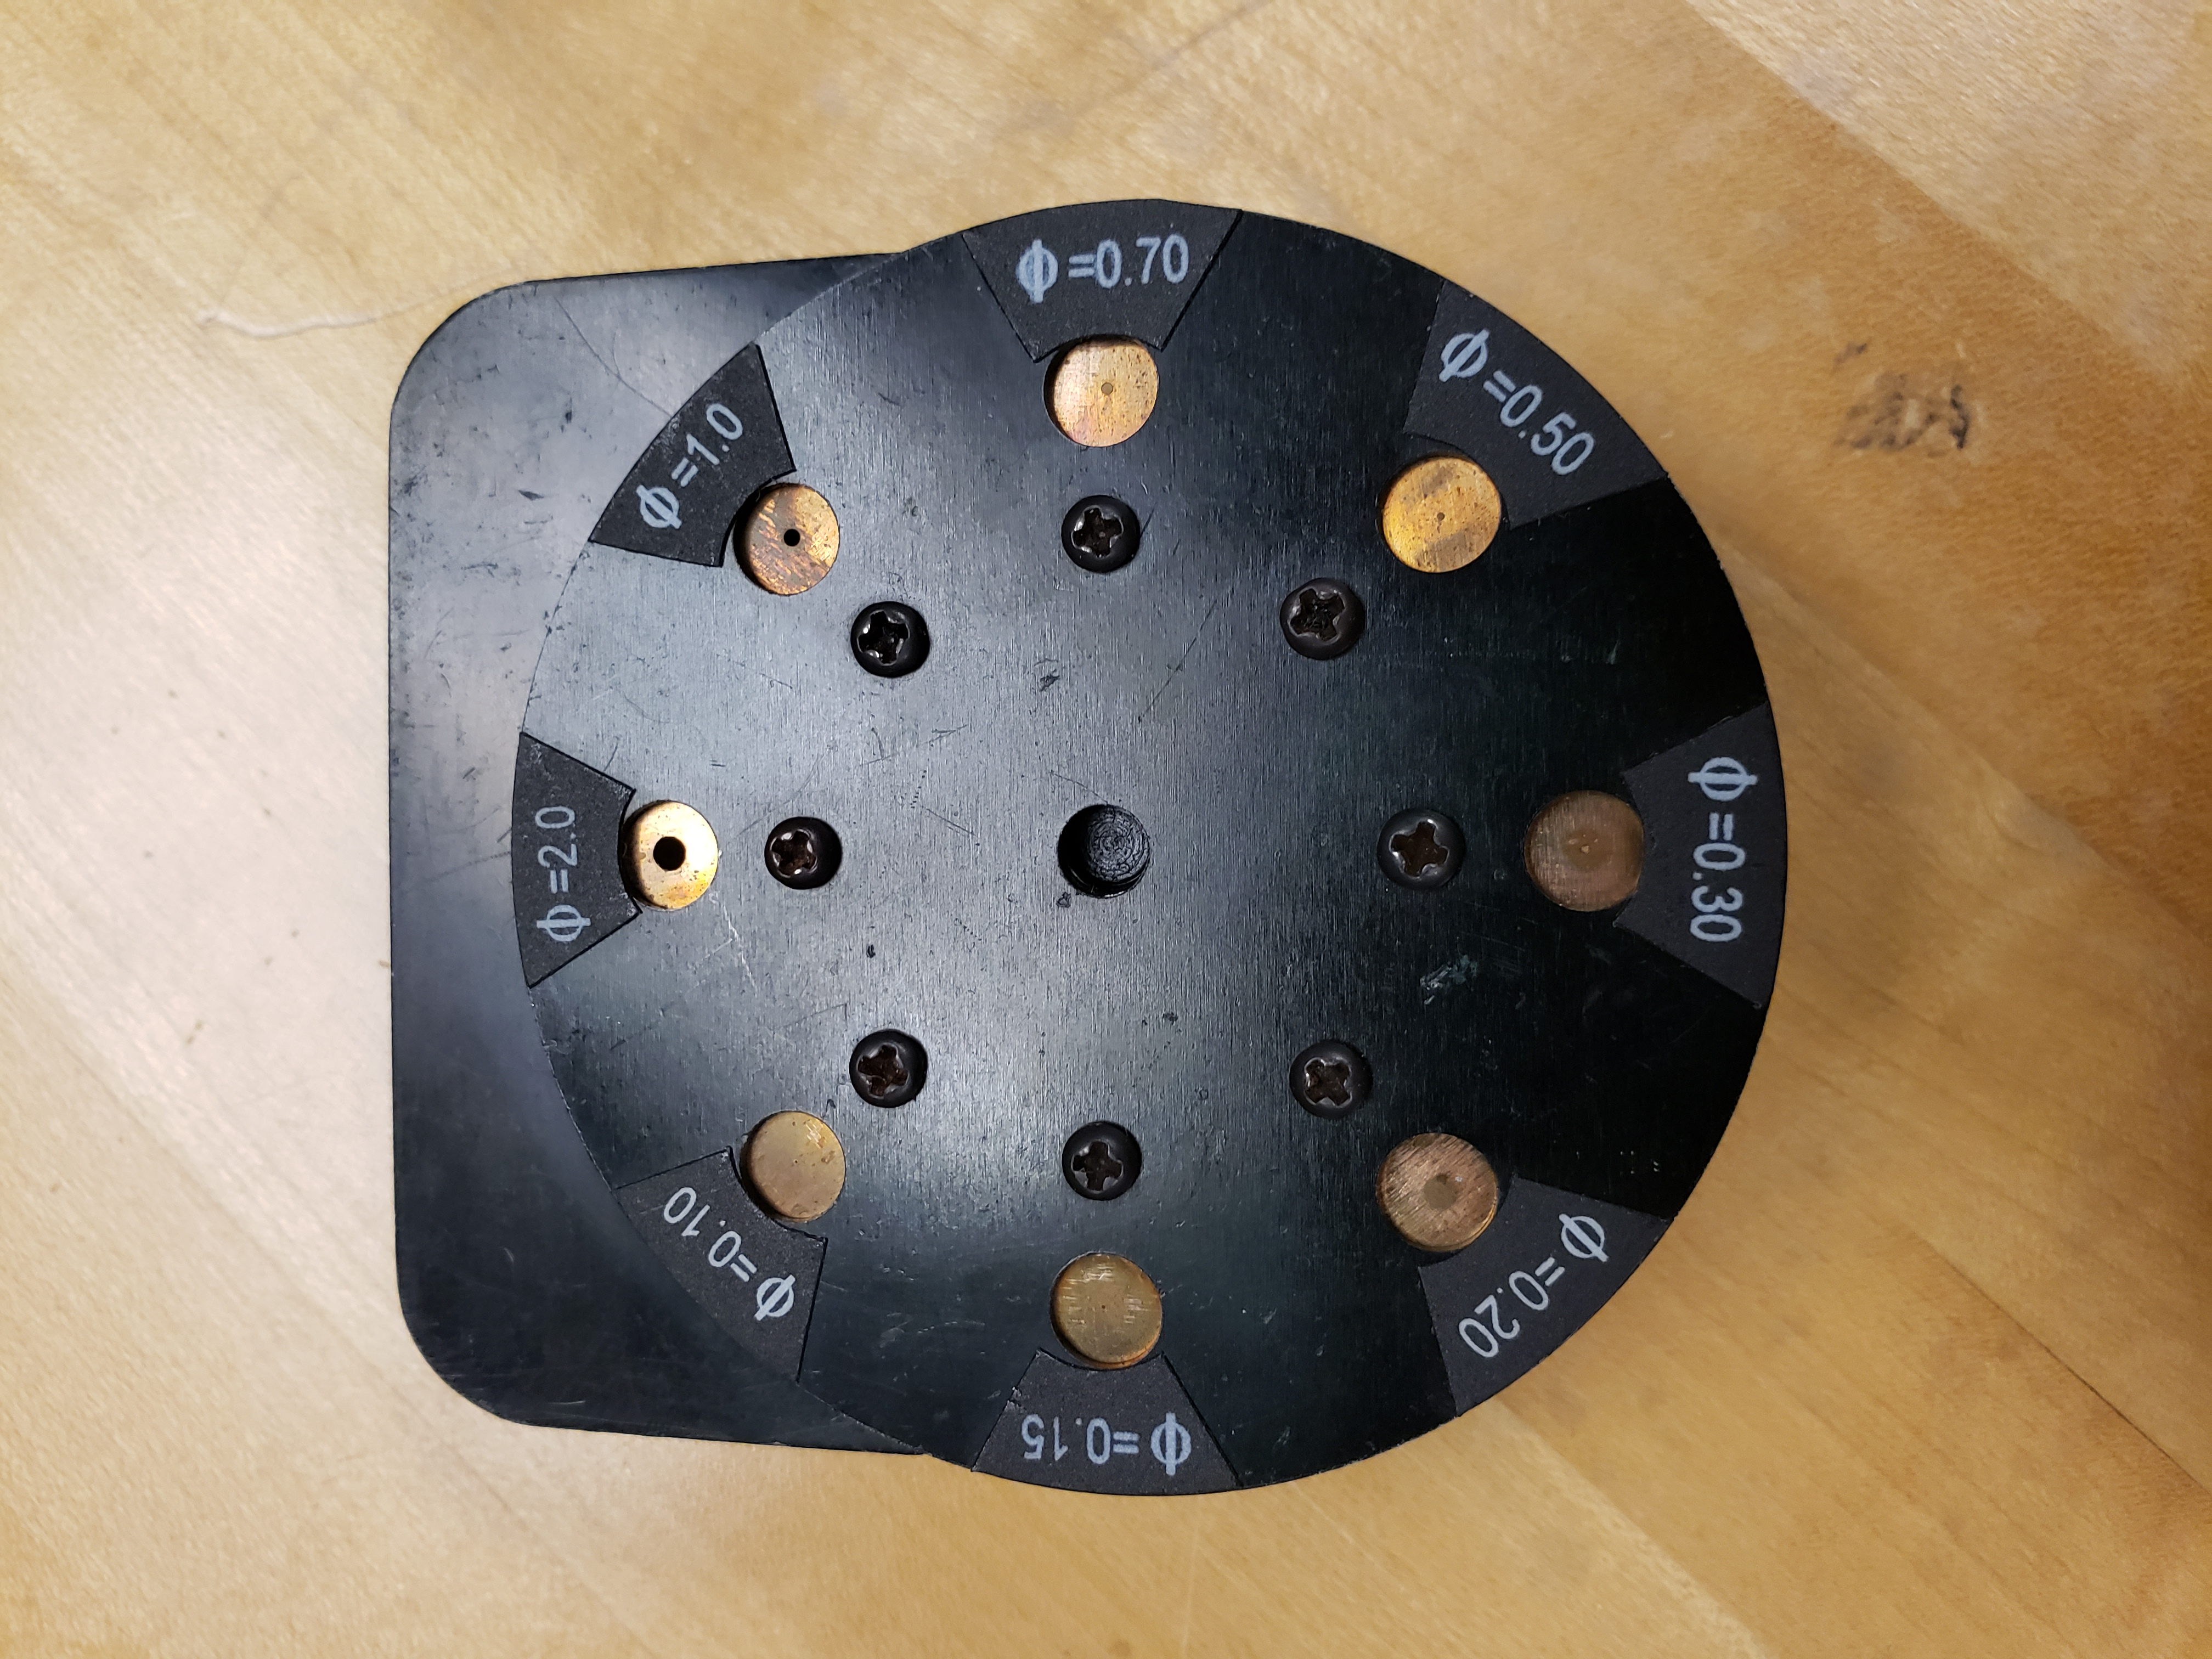
\includegraphics[ width = \linewidth ]{aperture.jpg}
    \caption{The variable aperture used. The numbers shown indicate the diameter (in mm) of the corresponding aperture}
    \label{fig:aperture}
\end{figure}
We placed the pinhole/variable aperture in the Fourier plane and the camera in the image plane. Once both objects were aligned, we then varied the aperture size and took a picture of the corresponding image with the camera. It should be noted that we observed the Fourier transform of filter 3 (shown in Figure \ref{fig:filters}) for this part of the lab.

\section{Measurements and Data Analysis}

\subsection{Data Collection}
\subsubsection{Observing the Fourier Transform}
As mentioned in the apparatus section, we used the camera, placed in the Fourier and image plane, to capture images of the Fourier and inverse Fourier transform, respectively. On top of that, we also used the camera to capture the image of the filter right as the laser passed through it. The images that we captured for this part of the lab can all be found in the Appendix; namely, parts A, B, and C.

Once we have the images, we then used Mathematica to calculate the Fourier transform of the image of the filter right as the laser passed through it. The resulting calculated Fourier transforms can all be found in the Appendix, part D.

\subsubsection{Observing How a Low-Pass Filter Affects the Fourier Transform}
Also mentioned in the apparatus section was how we captured the inverse Fourier transform with a pinhole/variable aperture involved. In short, we placed the camera in the image plane and captured the resulting images, which represent the inverse Fourier transform. As noted in the apparatus section, we used filter 3 for the entirety of this part of the lab.  
To study the effects of the low-pass filter on the Fourier transform, we used Mathematica to calculate the Fourier transform for each of the images that we got using various aperture diameters. 

\subsection{Data Analysis}
\subsubsection{Observing the Fourier Transform}
First, qualitative comparisons of the calculated Fourier Transform from Mathematica and the image at the Fourier Plane were done. We expect these images to be roughly identical. Additionally, qualitative comparisons of the captured image at the image plane (representing the inverse Fourier transform) and initial image after passing through the objects were done. As before, we expect these images to be roughly identical.

After validating that the image at Fourier Plane maintains the qualitative features of the Fourier Transform, we compared the image at the Fourier Plane with the theoretical Fourier Transform for filter 4. Filter 4 is an object consisting of horizontal lines of period 0.6mm as seen in Fig. \ref{fig:Line_Predict}a. Based on the shape of this object, we expected the Fourier Transform to be a vertical line, which was observed in the Fourier Plane as seen in Fig. \ref{fig:Line_Predict}b. Based on the theoretical discussion provided in the Optical Fourier Transform Produced by a Lens section in the introduction, we expected the peaks in the Fourier plane to be $\nu \lambda f$ apart. Given a spatial frequency of $\frac{5}{3}$ cycles per mm, a focal length of 300mm, and a laser wavelength of $632.8 \ \si{nm}$, we expected the peaks to be located $316.4 \mu m$ apart. Using ImageJ, an image processing software, we measured the distance in pixels between 16 peaks and converted to a distance based on the camera pixel resolution of $8.4\mu m$ per pixel. Fig. \ref{fig:Line_Predict}b shows the distances between pixels. A mean and standard error were calculated from these measurements. 

Additionally, the distance between lines was measured in the image plane, corresponding to the inverse Fourier transform of the Fourier transform, using ImageJ, with a mean and standard deviation calculated as before. These values were compared with the theoretical value of 0.6 mm given by the filter design. 

\subsubsection{Observing How a Low-Pass Filter Affects the Fourier Transform}
Apertures of various sizes ranging from 300 $\mu m$ in diameter to 2000 $\mu m$ diameter were placed in the Fourier Plane. Since we expected the placement of an aperture to act as a low pass filter, we computationally calculated the Fourier Transform of the captured image at the image plane. The physical distance between discernible features, illustrated with a blue line in Fig. \ref{fig:Pinhole}b, was measured in ImageJ and compared with the aperture size. We repeated the measurements 16 times to generate a mean and standard error. 

As low pass filters are often used in image blurring and smoothing, we attempted to quantify the impact aperture size had on the sharpness of the features. As shown in Fig. \ref{fig:Pinhole}c, the image gradient of the captured image in the image plane was calculated for each image \cite{feichtenhofer2013perceptual}. A region of interest around each edge was drawn and the mean value along 16 edges was measured. An example region of interest is illustrated by the orange circle in Fig. \ref{fig:Pinhole}c. It is noted that the units of edge gradient are in units of camera pixel intensity per pixel.

As we expect both the furthest distance between features in the calculated Fourier Transform and image sharpness to scale with aperature size, we did a linear fit of the these metrics as a function of aperture size using Python. Error bars in the data were based on the standard error. Uncertainty intervals for the fit were found by taking the uncertainty of fitted parameters, found from taking the square root of the diagonals of the covariance matrix. The plotted upper and lower bounds are the correspond to the 95 percent confidence interval for the fitted distribution, as twice the uncertainty in fitted parameters was used. 

\subsection{Results}

\subsubsection{Captured and Reconstructed Fourier Transform Agree Qualitatively}

First, we sought to verify whether or not the image at the focal plane of the lens indeed produced the Fourier Transform of an image. Fig. \ref{fig:Line_Predict2}c and Fig. \ref{fig:Line_Predict2}d show the image captured at the Fourier plane and the reconstructed Fourier transform of the original object shown in Fig. \ref{fig:Line_Predict2}a. Excellent qualitative similarities in the features between the computed Fourier transform and the image at the Fourier plane was observed. This was true for all six filters examined, where the image at the Fourier plane and computed Fourier transforms can be found in Appendix part B and D.

Next, we sought to compare the image at the Image plane (captures the inverse Fourier transform of the Fourier transform) with the image of the original object. Fig. \ref{fig:Line_Predict2}a Fig. \ref{fig:Line_Predict2}b show an image of the original object and the image at the image plan. As with the Fourier transform, excellent qualitative agreement is noted between the image at the image plane and original object. This was true for all six filters, where the original images and photos at the image plane can be found in Appendix part A and C.
\begin{figure}
    \centering
    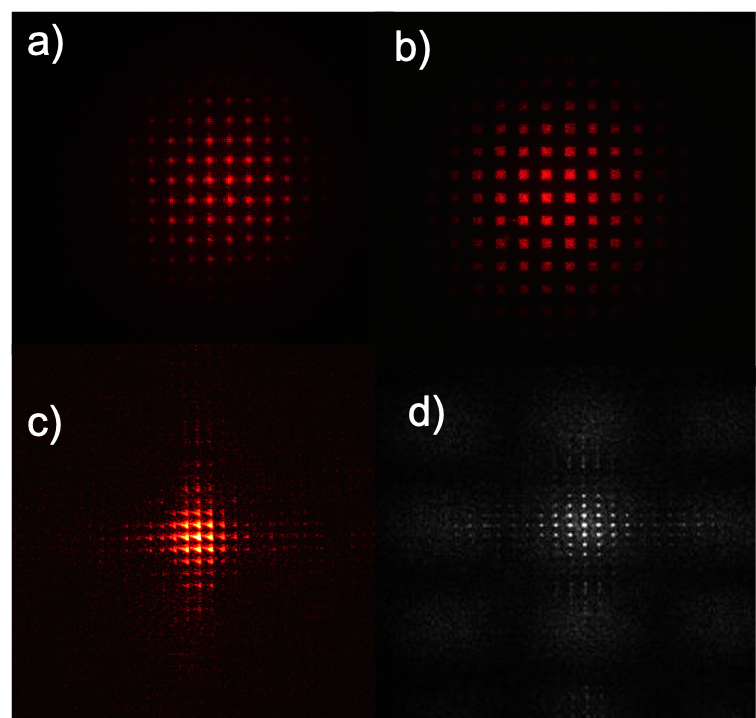
\includegraphics[ width = \linewidth ]{ReconstructionFFT.png}
    \caption{a) Original object after ND filters using filter 5. b) Image at image plane. c) Captured Fourier Transform at Fourier plane. d) Reconstructed Fourier Transform calculated from Mathematica.}
    \label{fig:Line_Predict2}
\end{figure}
\subsubsection{Comparison of Image at Fourier Plane with Predictions from the Paraxial Approximation}

Given the qualitative agreement between the image at the Fourier plane and computed Fourier Transform, we sought to quantitatively compare the two. For this purpose, we measured the distance between features in the Fourier plane and image plane and compared the distances with theoretical values. The object in \ref{fig:Line_Predict2}a shows the original image, which consist of horizontal lines separated by 0.6 mm. 
\begin{figure}
    \centering
    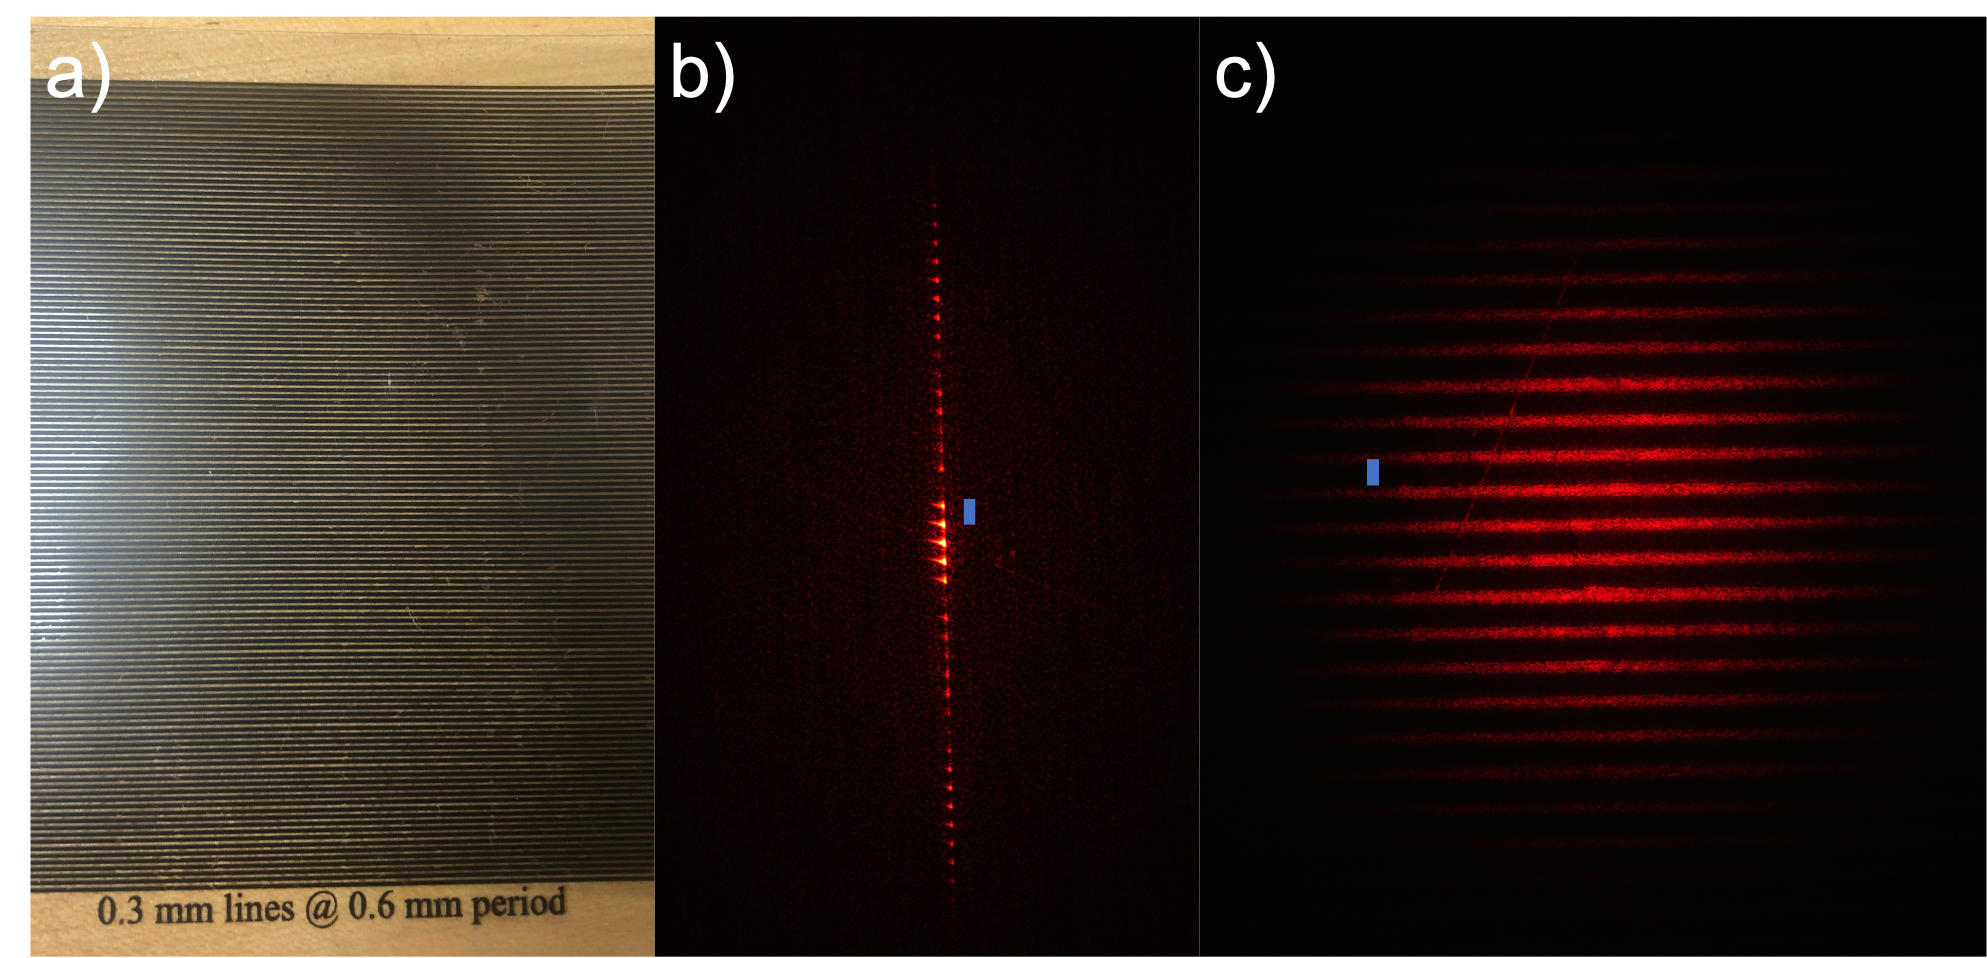
\includegraphics[ width = \linewidth ]{Predictions_Line.png}
    \caption{a) Original physical object using filter 4. b) Image at Fourier Plane. Blue bar shows distance between peaks in Fourier Plane. c) Reconstructed image after inverse Fourier Transform. Blue bar illustrates measurement of distance between lines.}
    \label{fig:Line_Predict}
\end{figure}
Fig. \ref{fig:Line_Predict2}b shows the image at the Fourier Plane, with a blue line drawn on to show the distance between peaks. As expected for this object, the image at the Fourier Plane was a vertical line with peaks spaced along that line. The distance between peaks was compared with the theoretical value (see section IV.B.1). The measured distance, shown in the table below, between peaks was consistent with the theoretically predicted value, with the difference within the standard error for the measured value. 

\begin{center}
\begin{tabular}{||c | c||} 
 \hline
  & Distance in Fourier Plane ($\mu m$)\\ [0.5ex]
 \hline
 Measured & 319.0 $\pm$ 21.4 \\ 
 \hline
 Predicted & 316.4  \\
 \hline
\end{tabular}
\end{center}

Fig. \ref{fig:Line_Predict2}b shows the image at the image plane (also called the Inverse Fourier Plane), with a blue line drawn on to show the distance between horizontal lines. We expect the distance to be the same as the spacing in the original object, which is 0.6 mm. The measured distance, shown in the table below, between peaks was consistent with the theoretically predicted value, with the difference less than the standard error for the measured value.

\begin{center}
\begin{tabular}{||c | c||} 
 \hline
  & Distance in Inverse Fourier Plane ($\mu m$)\\ [0.5ex]
 \hline
 Measured & 593 $\pm$ 16.3 \\ 
 \hline
 Predicted & 600  \\
 \hline
\end{tabular}
\end{center}

\subsubsection{Addition of Pinhole Acts as a Lowpass Filter}

After validating that image at the focal plane of the lens produces a Fourier transform, we added apertures of varying diameter at the focal plane. The addition of the aperture acts as a low pass filter by blocking the high frequency components in the Fourier Plane from contributing to the final image in the image plane. This reduces high spatial frequency features of the image in the image plane such as edges and acts to blur the image. To test this, we placed an aperture of various sizes at the Fourier Plane and captured photos of the image at the image plane. Fig. \ref{fig:aperture}a shows a photo at the image plane when a 2mm diameter aperture was used. The photos corresponding to different aperture sizes can be found in appendix E. As expected, the images become increasingly blurry as the aperture size decreased.  Additionally, the image becomes smaller with smaller apertures, consistent with the aperture blocking light at more oblique angles. These images are found in appendix E and the computed Fourier transforms are found in appendix F. 
\begin{figure}[H]
    \centering
    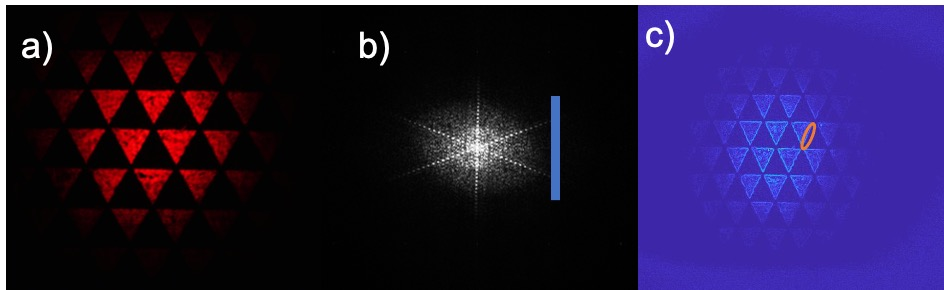
\includegraphics[ width = \linewidth ]{PinholeCalc.jpg}
    \caption{a) Captured image at image plane for 2mm diameter aperture using filter 3. b) Calculated Fourier Transform of image in a). Blue line represents diameter of Fourier Transform. c) Magnitude of image gradient of for image in a). Orange circle shows a region of interest used to calculate gradient at an edge.}
    \label{fig:Pinhole}
\end{figure}
Fig. \ref{fig:aperture}b shows the computed Fourier transform of Fig. \ref{fig:aperture}a. As expected, the size of the computed Fourier transform decreases with smaller apertures, consistent with the aperture acting as a low-pass filter.  To quantify the size of the Fourier transform, we quantified the distance between the furthest features in the computed Fourier transform (see IV.B.2). Fig. \ref{fig:aperture}c shows the gradient of Fig. \ref{fig:aperture}a. The value of the gradient along the edges was used to quantify how sharp the images of the edges were (see IV.B.2). These values are seen in the table below. As expected, both the computed Fourier transform diameter and edge gradient decreased with smaller aperture sizes. Such measurements are consistent with the image becoming more blurry with smaller apertures. Somewhat interestingly, the computed Fourier transform diameter was always bigger than the aperture diameter even though one would expect them to be the same size. It is unclear what the exact reason for this although optical aberrations, measurement errors, and aliasing present in the discrete Fourier transform may be contributing factors. 

\begin{center}
\begin{tabular}{||c | c | c||} 
 \hline
  Aperture Diam ($\mu m$) &  FFT Diam ($\mu m$) &  Edge Gradient\\ [0.5ex] 
 \hline
 No Aperture & 5113.5 $\pm$ 181.4 & 114.3 $\pm$ 25.7 \\ 
 \hline
 2000 &  2307.9 $\pm$ 98.7 & 52.5 $\pm$ 14.3\\
 \hline
 1000 &  1107.1 $\pm$ 39.9 & 24.3 $\pm$ 4.8\\
 \hline
 700 &  987.0 $\pm$ 27.8 & 17.2 $\pm$ 3.9\\
 \hline
 500 &  705.6 $\pm$ 23.1 & 14.8 $\pm$ 2.9\\
 \hline
 300 & 456.1 $\pm$ 14.1 & 10.1 $\pm$ 2.6\\
 \hline
\end{tabular}
\end{center}

A linear fit between FFT diameter and Aperture diameter is plotted in Fig. \ref{fig:ApertureDiam}. A linear fit represents the data fairly well. The error fitted line is within the error bar, corresponding to the standard error, for each of the measurements. This provides good indication that the aperture is indeed filtering out higher frequency components in the Fourier plane. Further, the linear relation suggests that the frequencies filtered out are approximately linearly scaled with aperture diameter as one would expect.
\begin{figure}[H]
    \centering
    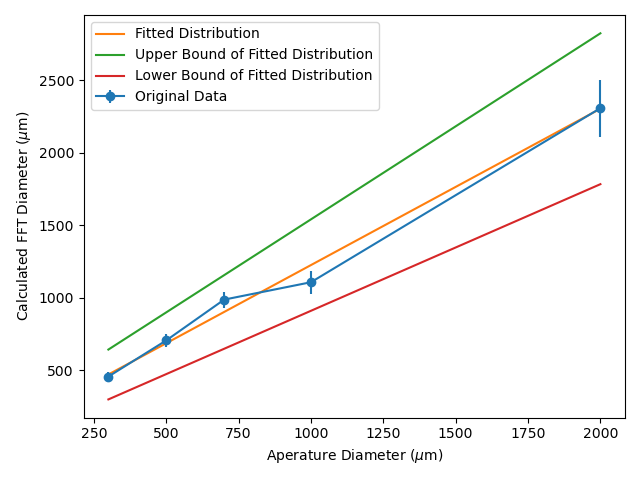
\includegraphics[ width = \linewidth ]{AperatureDiam.png}
    \caption{Diameter of the Fourier Transform plotted as a function of aperture diameter. Linear fit of data plotted. Error bars on data correspond to twice the standard error. Upper and lower bounds of fit correspond to twice the uncertainty in fitted parameters, found by taking the square root of the diagonals of the covariance matrix.}
    \label{fig:ApertureDiam}
\end{figure}
A linear fit between FFT diameter and edge gradient is plotted in Fig. \ref{fig:Edge}. A linear fit represents the data fairly well, with the error bars interesting with the linear fit. This shows that addition of an aperture indeed makes features less sharp, consistent with high frequency features being filtered out.
\begin{figure}
    \centering
    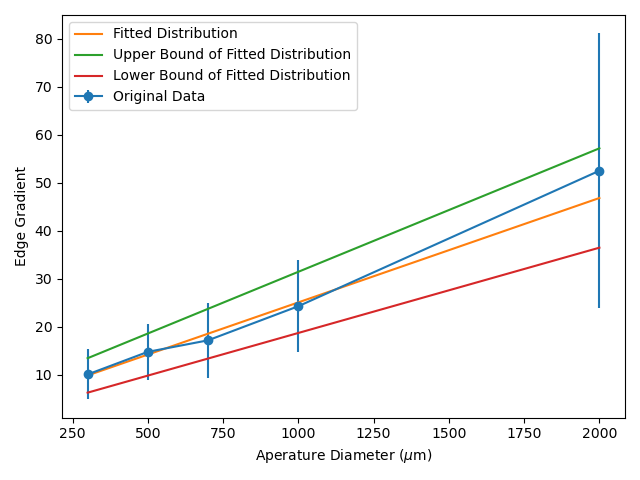
\includegraphics[ width = \linewidth ]{EdgeGradient.png}
    \caption{Edge gradient of image plotted as a function of aperture diameter. Linear fit of data plotted. Error bars on data correspond to twice the standard error. Upper and lower bounds of fit correspond to twice the uncertainty in fitted parameters, found by taking the square root of the diagonals of the covariance matrix.}
    \label{fig:Edge}
\end{figure}
\subsubsection{Reconstructed Fourier Transform Includes Aliasing}

One additional extra feature interesting featured noted was the presence of aliasing when reconstructing the Fourier transform using Mathematica. Fig. \ref{fig:Aliasing} shows the log of the computed Fourier transform of filter 3 to provide additional contrast. We note the presence of aliasing, as seen in the blue circles. If one extends the image, this aliasing was seen in a periodic pattern along both patterns. Aliasing is a feature present in the discrete Fourier Transform due to the finite sampling resolution and portrays low frequency components as higher frequency components. Of note, the image at the Fourier plane does not include aliasing, since the lens acts as a continuous Fourier Transform rather than a discrete Fourier Transform \cite{winograd1978computing}. 
\begin{figure}
    \centering
    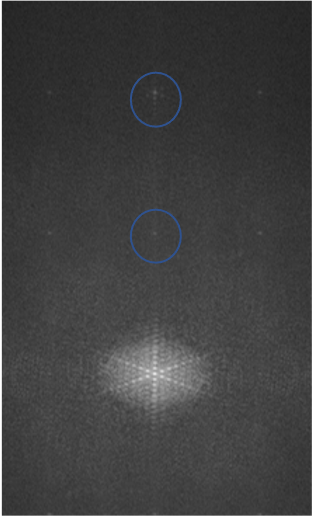
\includegraphics[ width = \linewidth ]{Aliasing.png}
    \caption{Calculated Fourier Transform on log scale using filter 3. Blue circles show 2 examples of aliasing, a result of the discretization involved in the discrete Fourier Transform calculation.}
    \label{fig:Aliasing}
\end{figure}

\section{Discussion}
Our results are largely consistent with theoretical predictions. First, great qualitative agreement was noted between the image at the Fourier Plane and computed Fourier Transform. This suggests that the lens does indeed act as a Fourier Transform when viewed at the Fourier Plane and that the Fourier Transform can be used to model what objects look like at the different planes of an optical system.

Additionally, the image of filter 4 at the focal plane matched well with quantitative observations. The theoretically predicted distances between peaks in the focal plane was $316.4 \mu m$ while the measured distance was $319.0 \pm 21.4 \mu m$, within the standard error to the predicted value. Similarly, the distance between lines in the inverse Fourier Transform plane was  $593.0 \pm 16.3 \mu m$, within a standard error the ground truth value of $600.0 \mu m$. This further suggests that Fourier optics not only qualitatively predicts the shape of a beam within different planes in an optical system, but can also be used to make quantitative assessments. It was somewhat interesting to note that the standard error of measurements of distance between lines in the inverse Fourier plane was smaller between peaks in the Fourier plane despite having a larger value. When manually drawing lines between objects of interest in both of these planes, we found more variation in the distance between features in the Fourier plane. This suggests some optical aberrations may be present in the Fourier plane. One example aberration is Petzval field curvature. The "focal plane" of a lens is not truly a plane but actually a curved surface. Our camera only captures images at a flat plane, meaning that distortions in the focal "plane" to this flat plane may distort the position of the features. Furthermore, distortion is another aberration that would particularly impact measurements. In cases of distortion, the distance of a point to the optical axis is does not scale linearly with the true physical distance of the object prior to the lens. Spherical aberration is another aberration that may be important, as the shape of the lens surface may refract off axis rays differently. Other aberrations that may be present include but are not limited to tilt and astigmatism. One could address these issues with different optical equipment. For example, aspheric lenses can be used to minimize spherical aberration. However, the trade off between cost and buying lenses to minimize aberrations ought to be considered. 

Another factor impacting quantitative measurements of the Fourier transform is if the camera was not placed exactly at the Fourier plane, the focal plane of the lens. Based on the paraxial transform, we would expect deviations of camera position from the focal plane to change the scaling of the distance between features. Further, it is possible that the camera may be tilted such that some parts of the camera are more in focus than others, which would asymmetrically magnify features. However, given the quantitative agreement between distances between peaks described earlier, we believe that the camera was positioned relatively well with respect to the focal plane. One experimental way to adjust for such errors could be placing the camera on a translation and rotational mount. After placement of the camera, a motor could be used to automatically translate and rotate the camera slightly. An image could be taken after each translation and rotation and the image with the best quantitative agreement with the real Fourier Transform could be deemed the optimal position of the camera.

Moreover, we examined the impact of adding an aperture to the focal plane on the image at the image plane. It was determined that placement of an aperture acts as a low pass filter. Qualitative observations of the image with smaller aperture sizes showed more blurry filters. A Fourier transform of these images show that the width of the features in the Fourier plane was reduced. This illustrates that the aperture was indeed cutting off high frequency components of the image. The edge gradient of the captured image was used to represent the sharpness of features. We found that edge gradient decreased with smaller apertures, suggesting that smaller apertures blur features as expected for a low-pass filter. The fits between aperture size versus FFT diameter and aperture size versus edge gradient were well modeled with a linear fit, with the the standard error of the measurements intersecting with the linear fit. This indicates that the cutoff frequency for the low-pass filter scales linearly with aperture diameter as one would expect if the image at the Fourier plane was truly the Fourier transform of the image. 

One source of error in this analysis was that the computed Fourier transform rather than the measured Fourier transform was used in this case. The computed Fourier transform has aliasing due to the discretization of the the signal. Indeed, we observed aliasing in our computed Fourier Transforms. An alternative method would be to test this would be to create the theoretical Fourier transform of the object and apply a digital low pass filter before performing an inverse Fourier transform to compare with the captured images. Another large source of error is perfect alignment of the center pinhole with the center of the optical axis. This would result in the pinhole asymmetrically cutting off frequencies about the origin of the Fourier transform, making the effect of the pinhole much more complication than a simple low-pass filter. Indeed, we found this problem to be particularly large when apertures sizes of less than $300 \mu m$ in diameter were used. One method for aligning the aperture as close to the center of the optical axis as possible would be to place a power meter directly behind the aperture at the focal plane and adjust the position of the aperture until power on that power meter was maximized. Finally, edge gradient is an imperfect measurement of image sharpness and other methods exist. One could choose to test those additional methods.  

Another method of improving the experiment would be to increase the size of the collimated beam input to the physical object. As seen in appendix A, the light passing initial object did not completely illuminate the camera as the beam spot was too small. This makes computing the theoretical Fourier Transform of the object very difficult as the true Fourier Transform would have to take into account the nonuniform beam profile. We measured the collimated beam diameter to be approximately 14mm, indicating that the lenses we choose to place before the diffuse object magnified the input light by about 20 times (input laser diameter is about 0.7 mm in diameter \cite{laser}). The focal lengths of the set of lenses before the object could be tuned to provide an even greater magnification.

\section{Conclusion}
We have discussed how a lens produces the Fourier transform of an object at its Fourier plane, and the key condition that we had to utilize was the paraxial approximation. We have also discussed how the propagation of light away from the Fourier plane to the second focusing lens produces the inverse Fourier Transform. Putting all this discussion into play, we utilized a "4-$f$" Fourier transform apparatus (as shown in Figure \ref{fig:app_schem}) to observe the Fourier and inverse Fourier Transform of various filters (all of which can be shown in Figure \ref{fig:filters}) produced from our lenses. With the help of Mathematica, we were able to calculate the expected Fourier transform of each of the filters, which allowed for us to verify whether or not the image we captured at the Fourier plane was indeed the Fourier transform of our filter.
Finally, we were also able to observe how a low-pass filter (which we emulated using a variable pinhole/aperture) affected the Fourier Transform of our filter by looking at the resulting image formed at the image plane. While we were able to show that the lenses in the "4-$f$" system acts as a Fourier Transform, there are several ways the data quality in this lab could be improved. One method would be to choose lens to reduce aberrations in the Fourier plane. Another method would be to choose optics with suitable focal lengths to expand the diameter of the input beam, so that one could calculate the theoretical Fourier Transform of the objects without needing to worry about beam profile.

\bibliographystyle{unsrt}
\bibliography{References}

\clearpage
\onecolumngrid
\section{Appendix}
Figure \ref{fig:filters} shows the corresponding filters that each of the images in this appendix refers back to.

\subsection{Captured Filter Image}
\begin{figure}[H]
    \centering
    \begin{minipage}{0.45\textwidth}
        \centering
        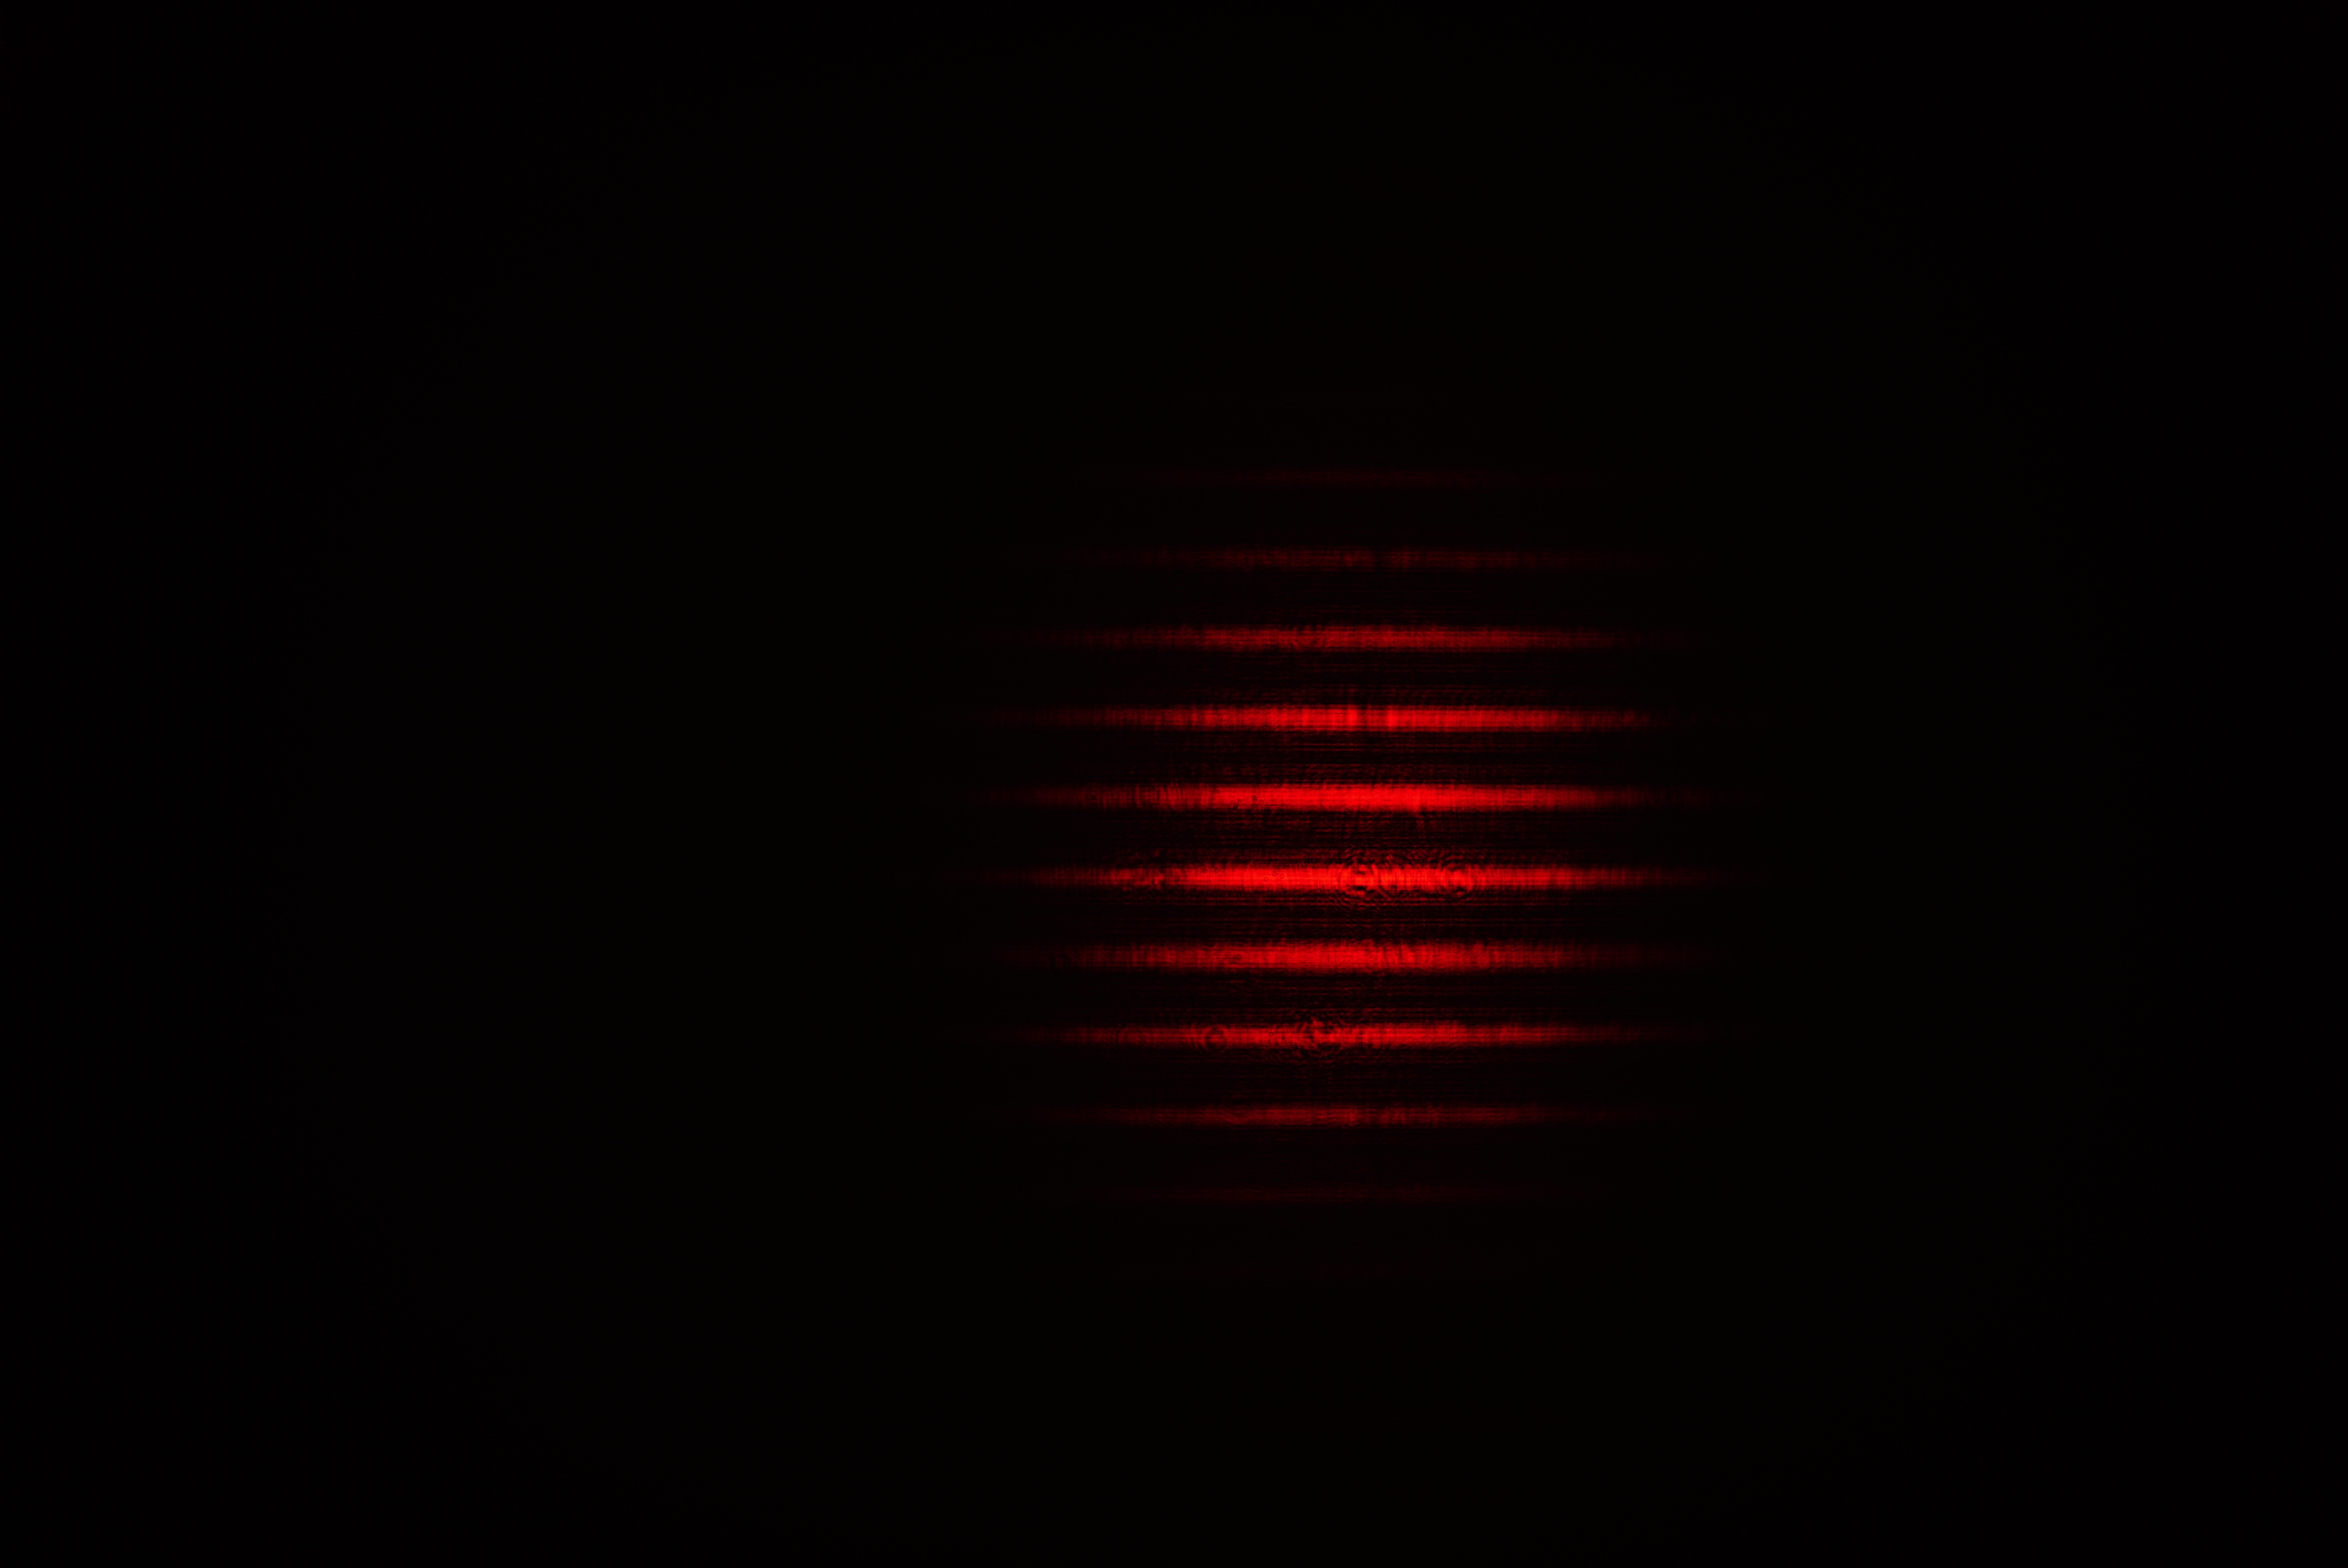
\includegraphics[ width = 0.95 \linewidth ]{figures/FilterImage/DSC01505.JPG}
        \caption{The captured image using filter 1}
    \end{minipage}%
    \begin{minipage}{0.45\textwidth}
        \centering
        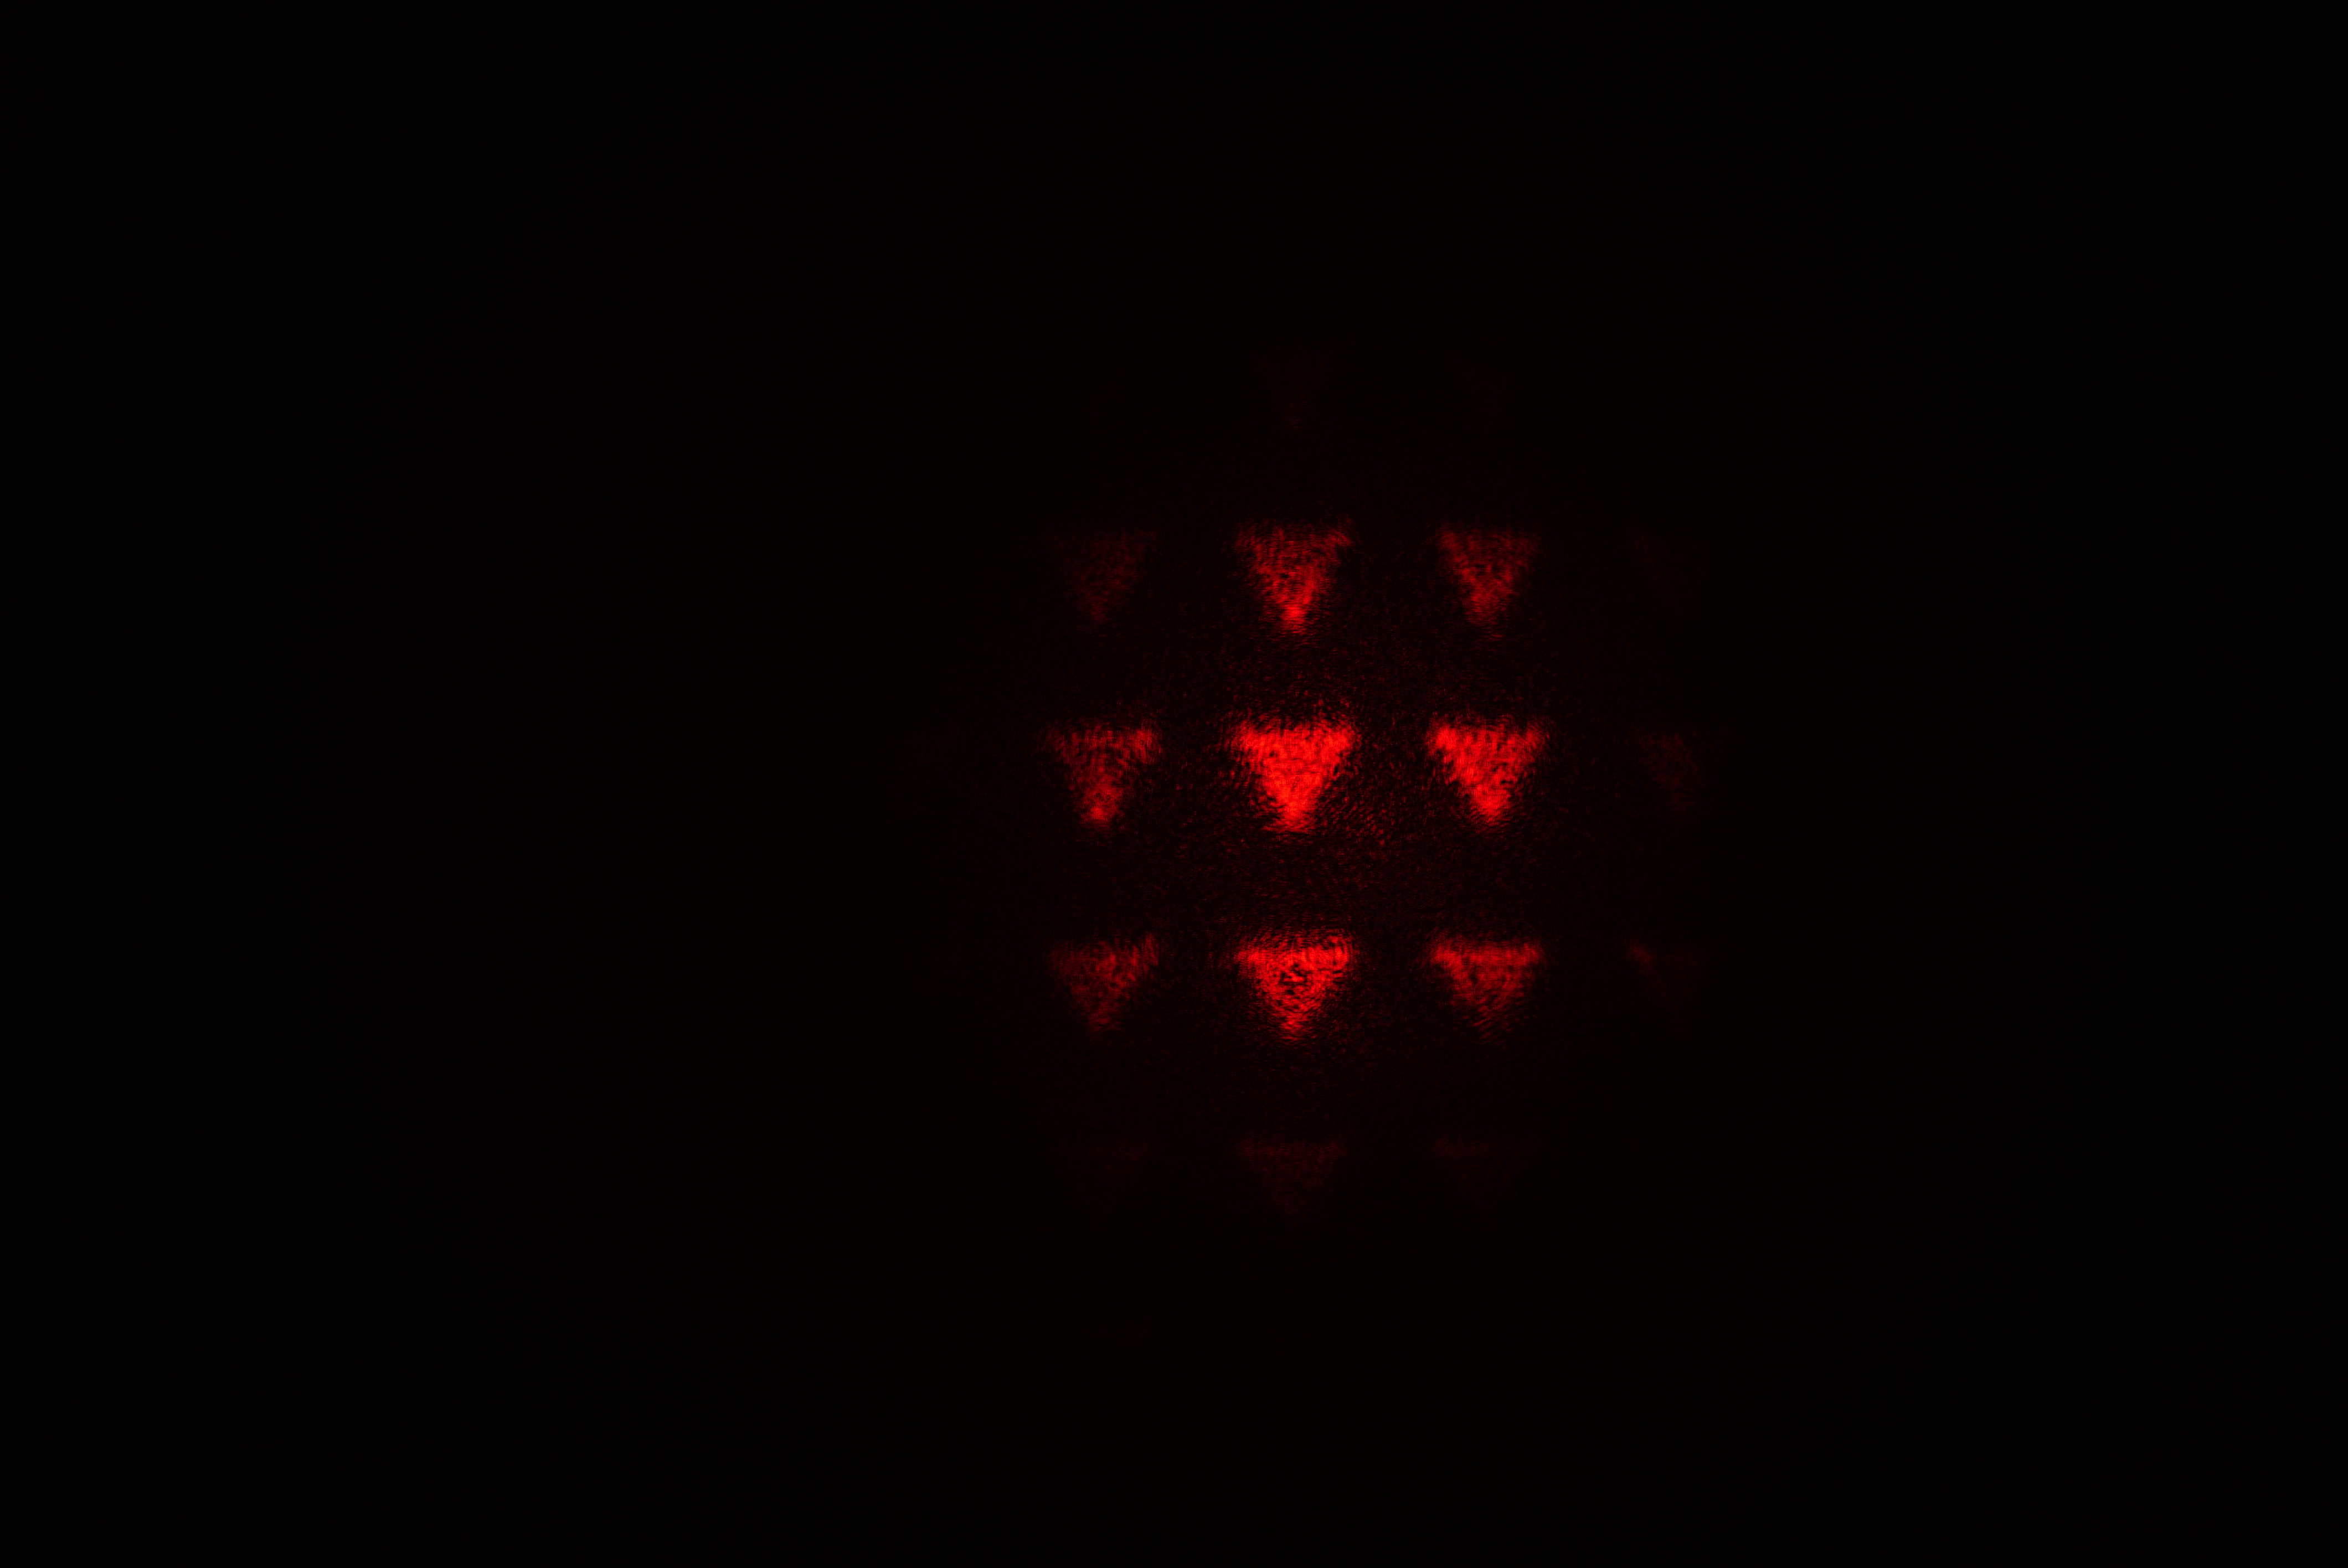
\includegraphics[ width = 0.95 \linewidth ]{figures/FilterImage/DSC01508.JPG}
        \caption{The captured image using filter 2}
    \end{minipage}%
    \vspace{1cm}
    \begin{minipage}{0.45\textwidth}
        \centering
        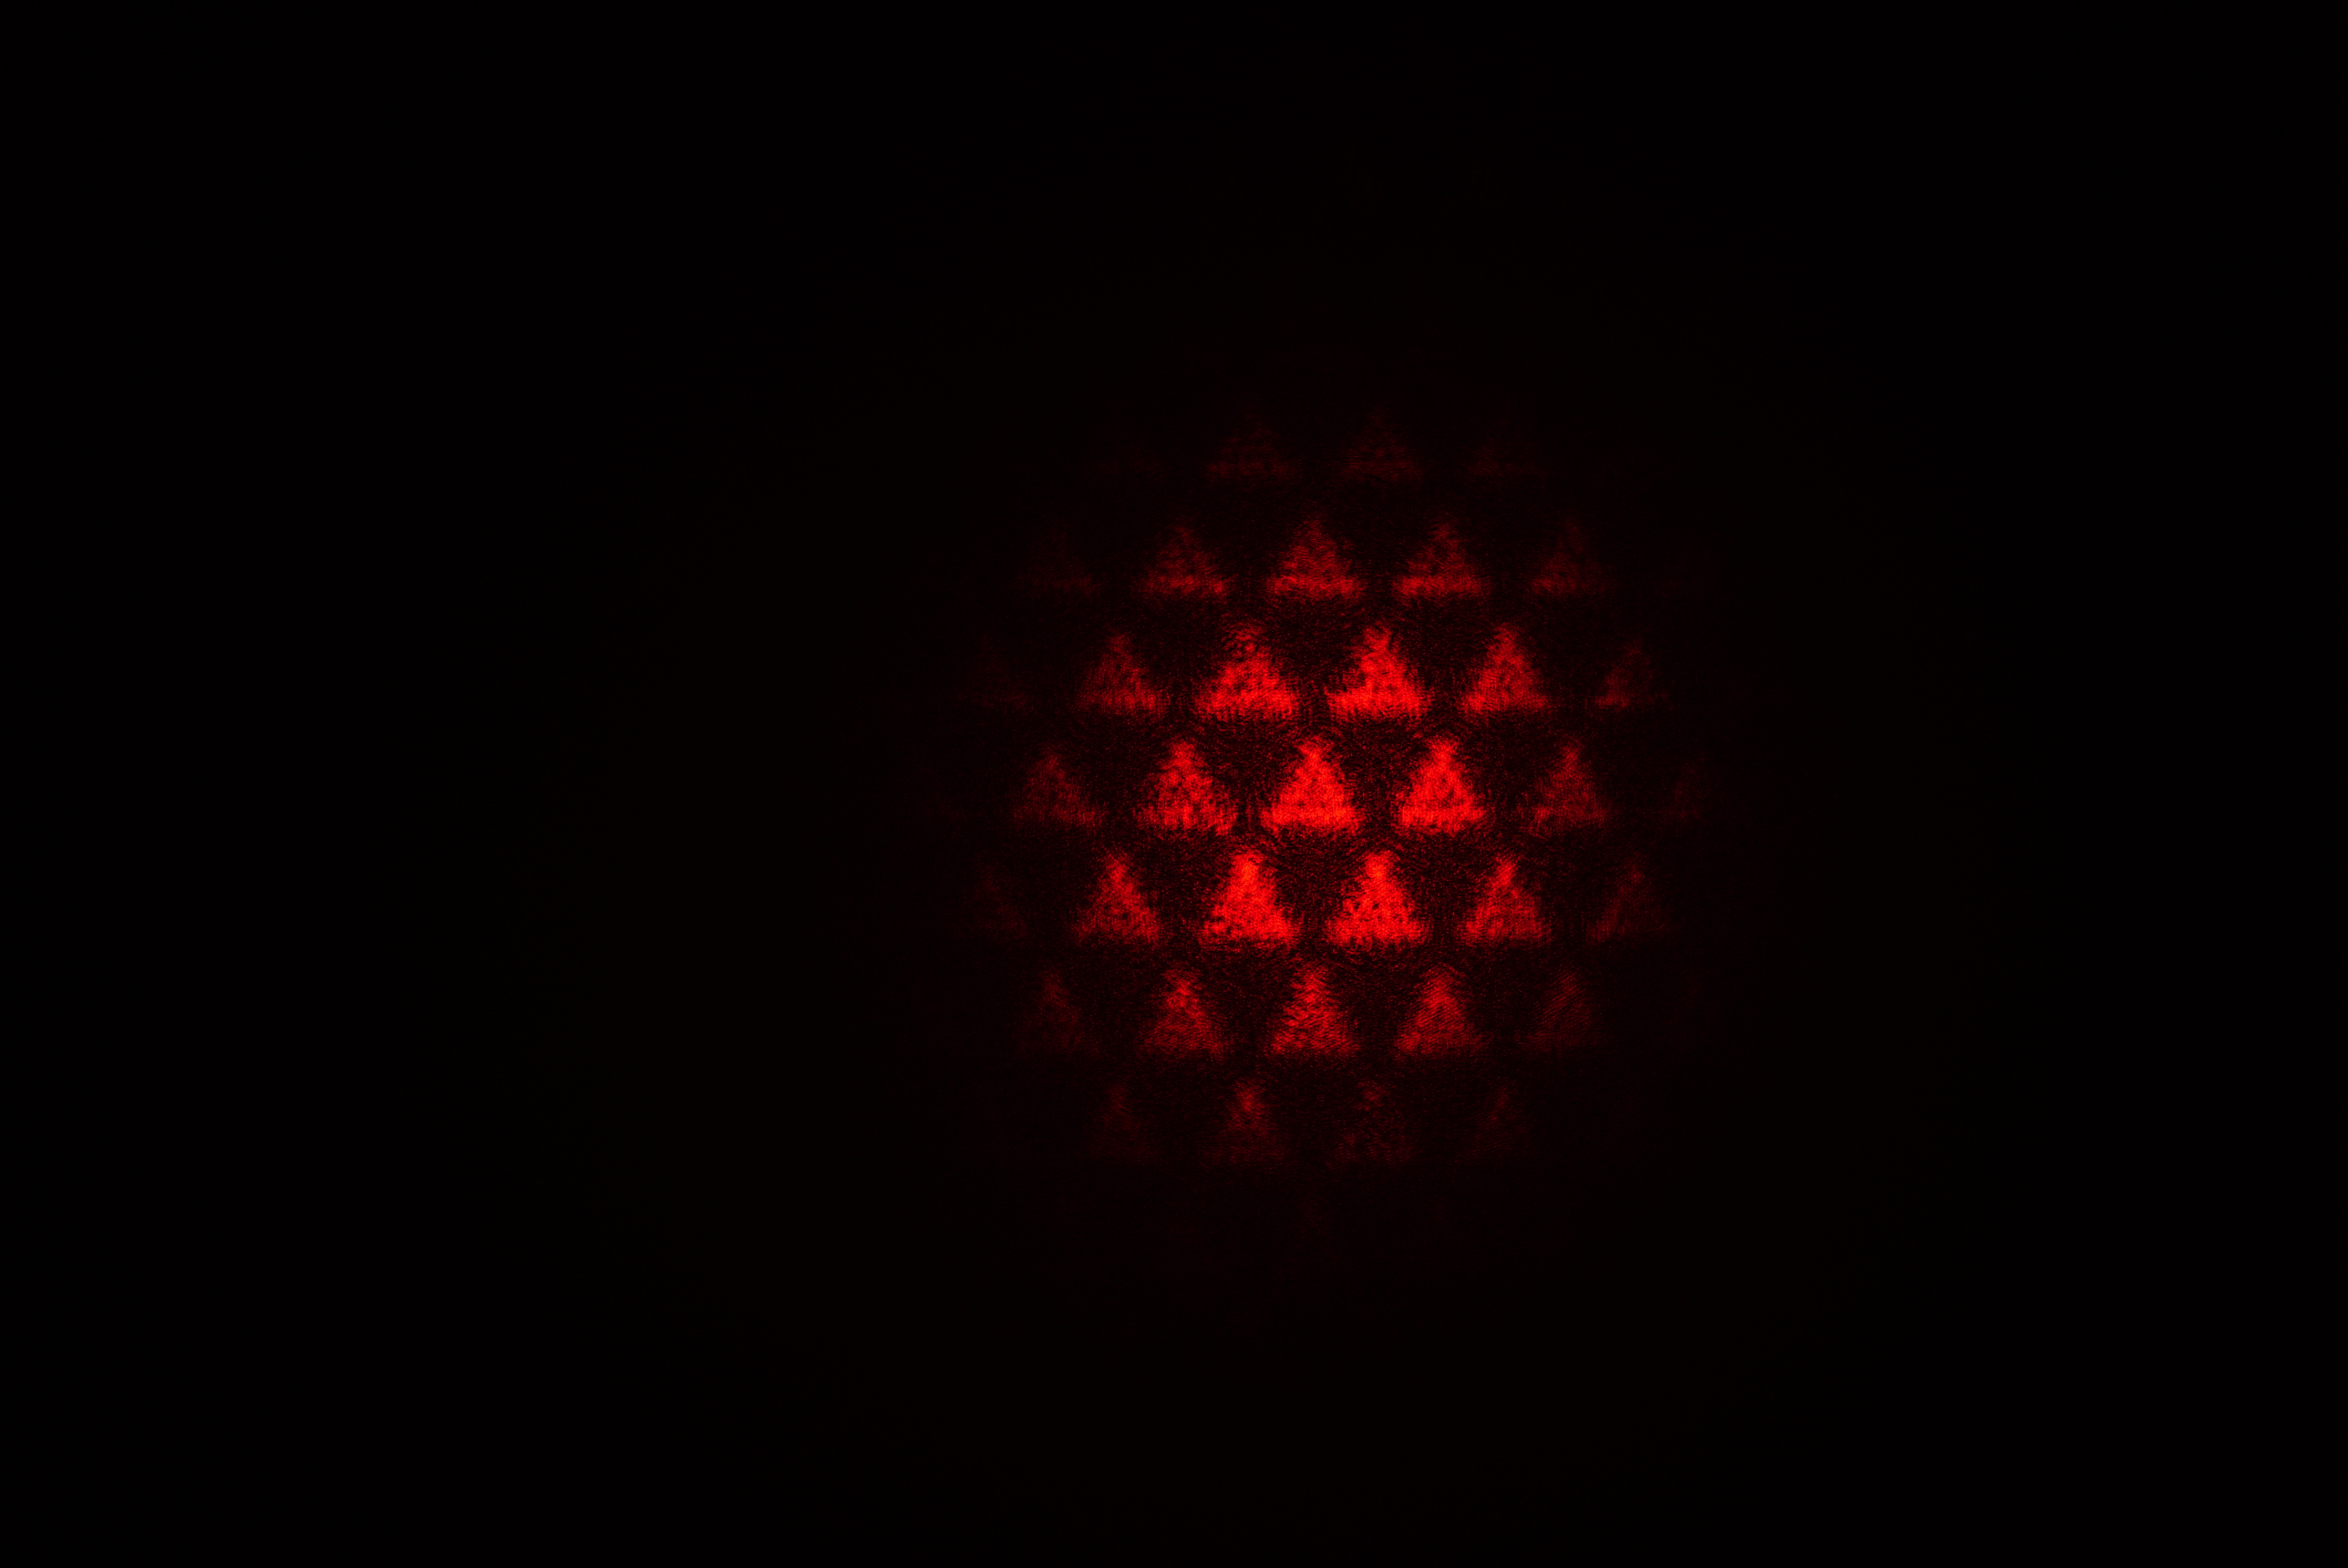
\includegraphics[ width = 0.95 \linewidth ]{figures/FilterImage/DSC01511.JPG}
        \caption{The captured image using filter 3}
    \end{minipage}%
    \begin{minipage}{0.45\textwidth}
        \centering
        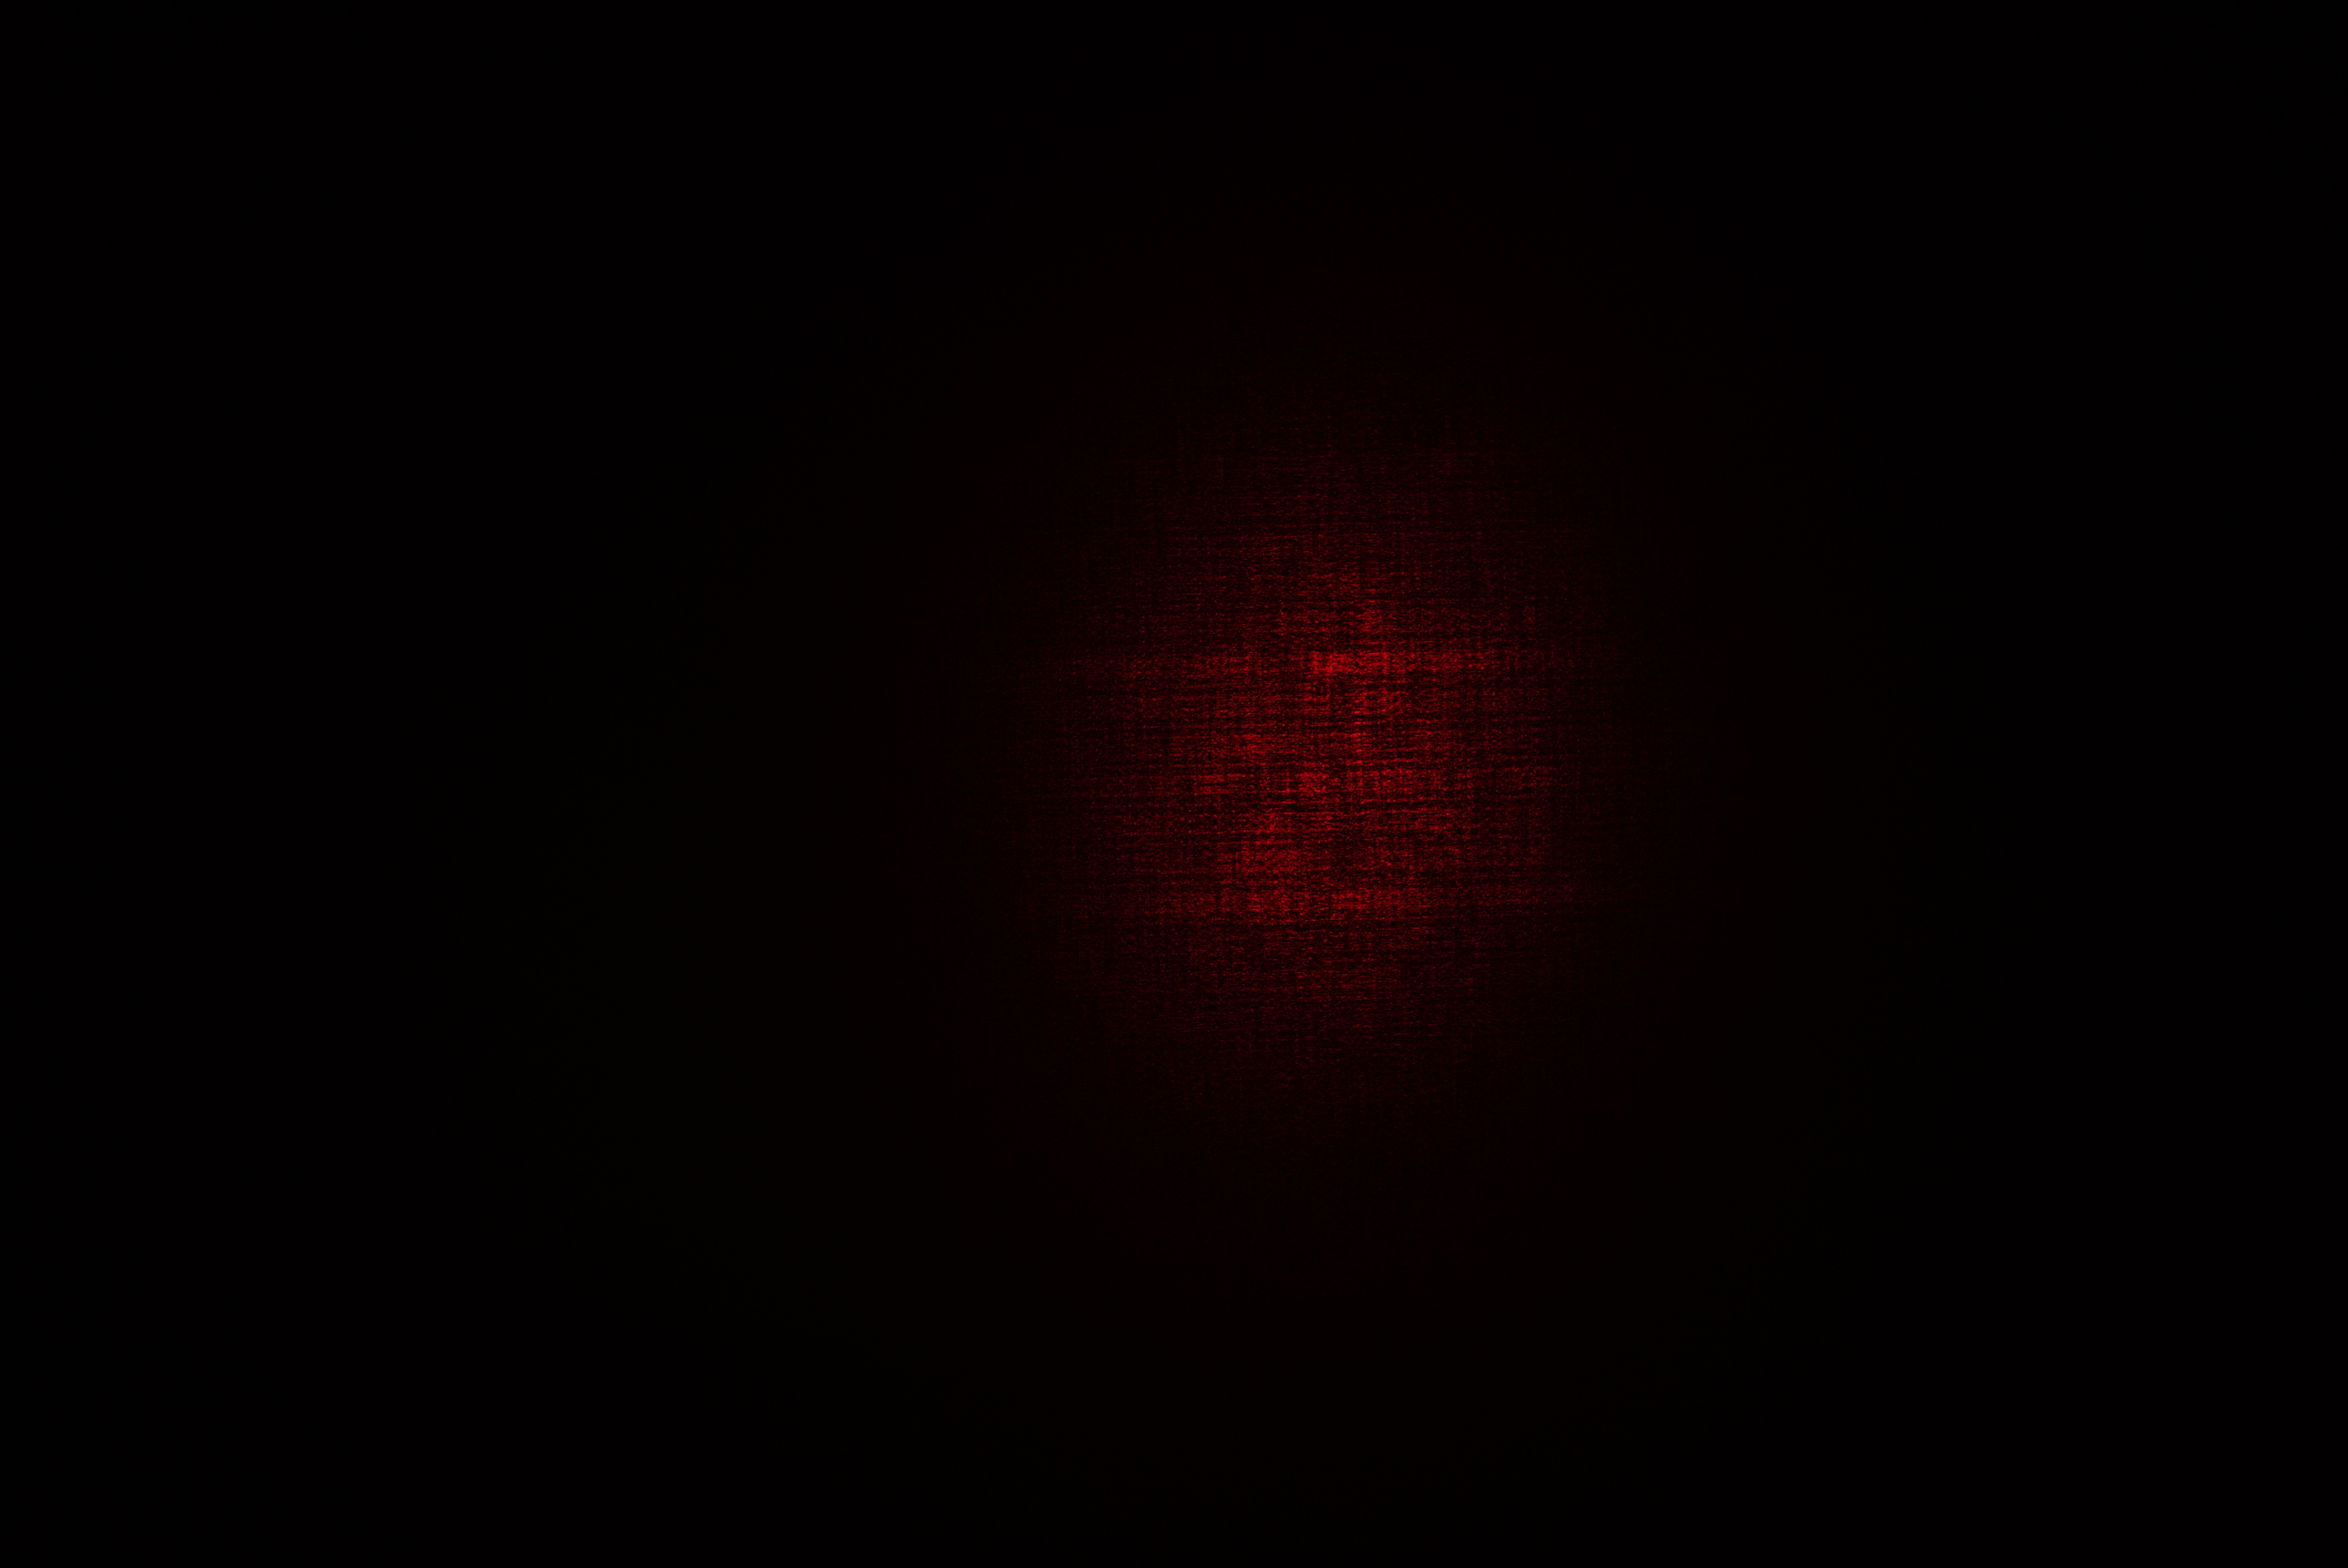
\includegraphics[ width = 0.95 \linewidth ]{figures/FilterImage/DSC01514.JPG}
        \caption{The captured image using filter 4}
    \end{minipage}%
    \vspace{1cm}
    \begin{minipage}{0.45\textwidth}
        \centering
        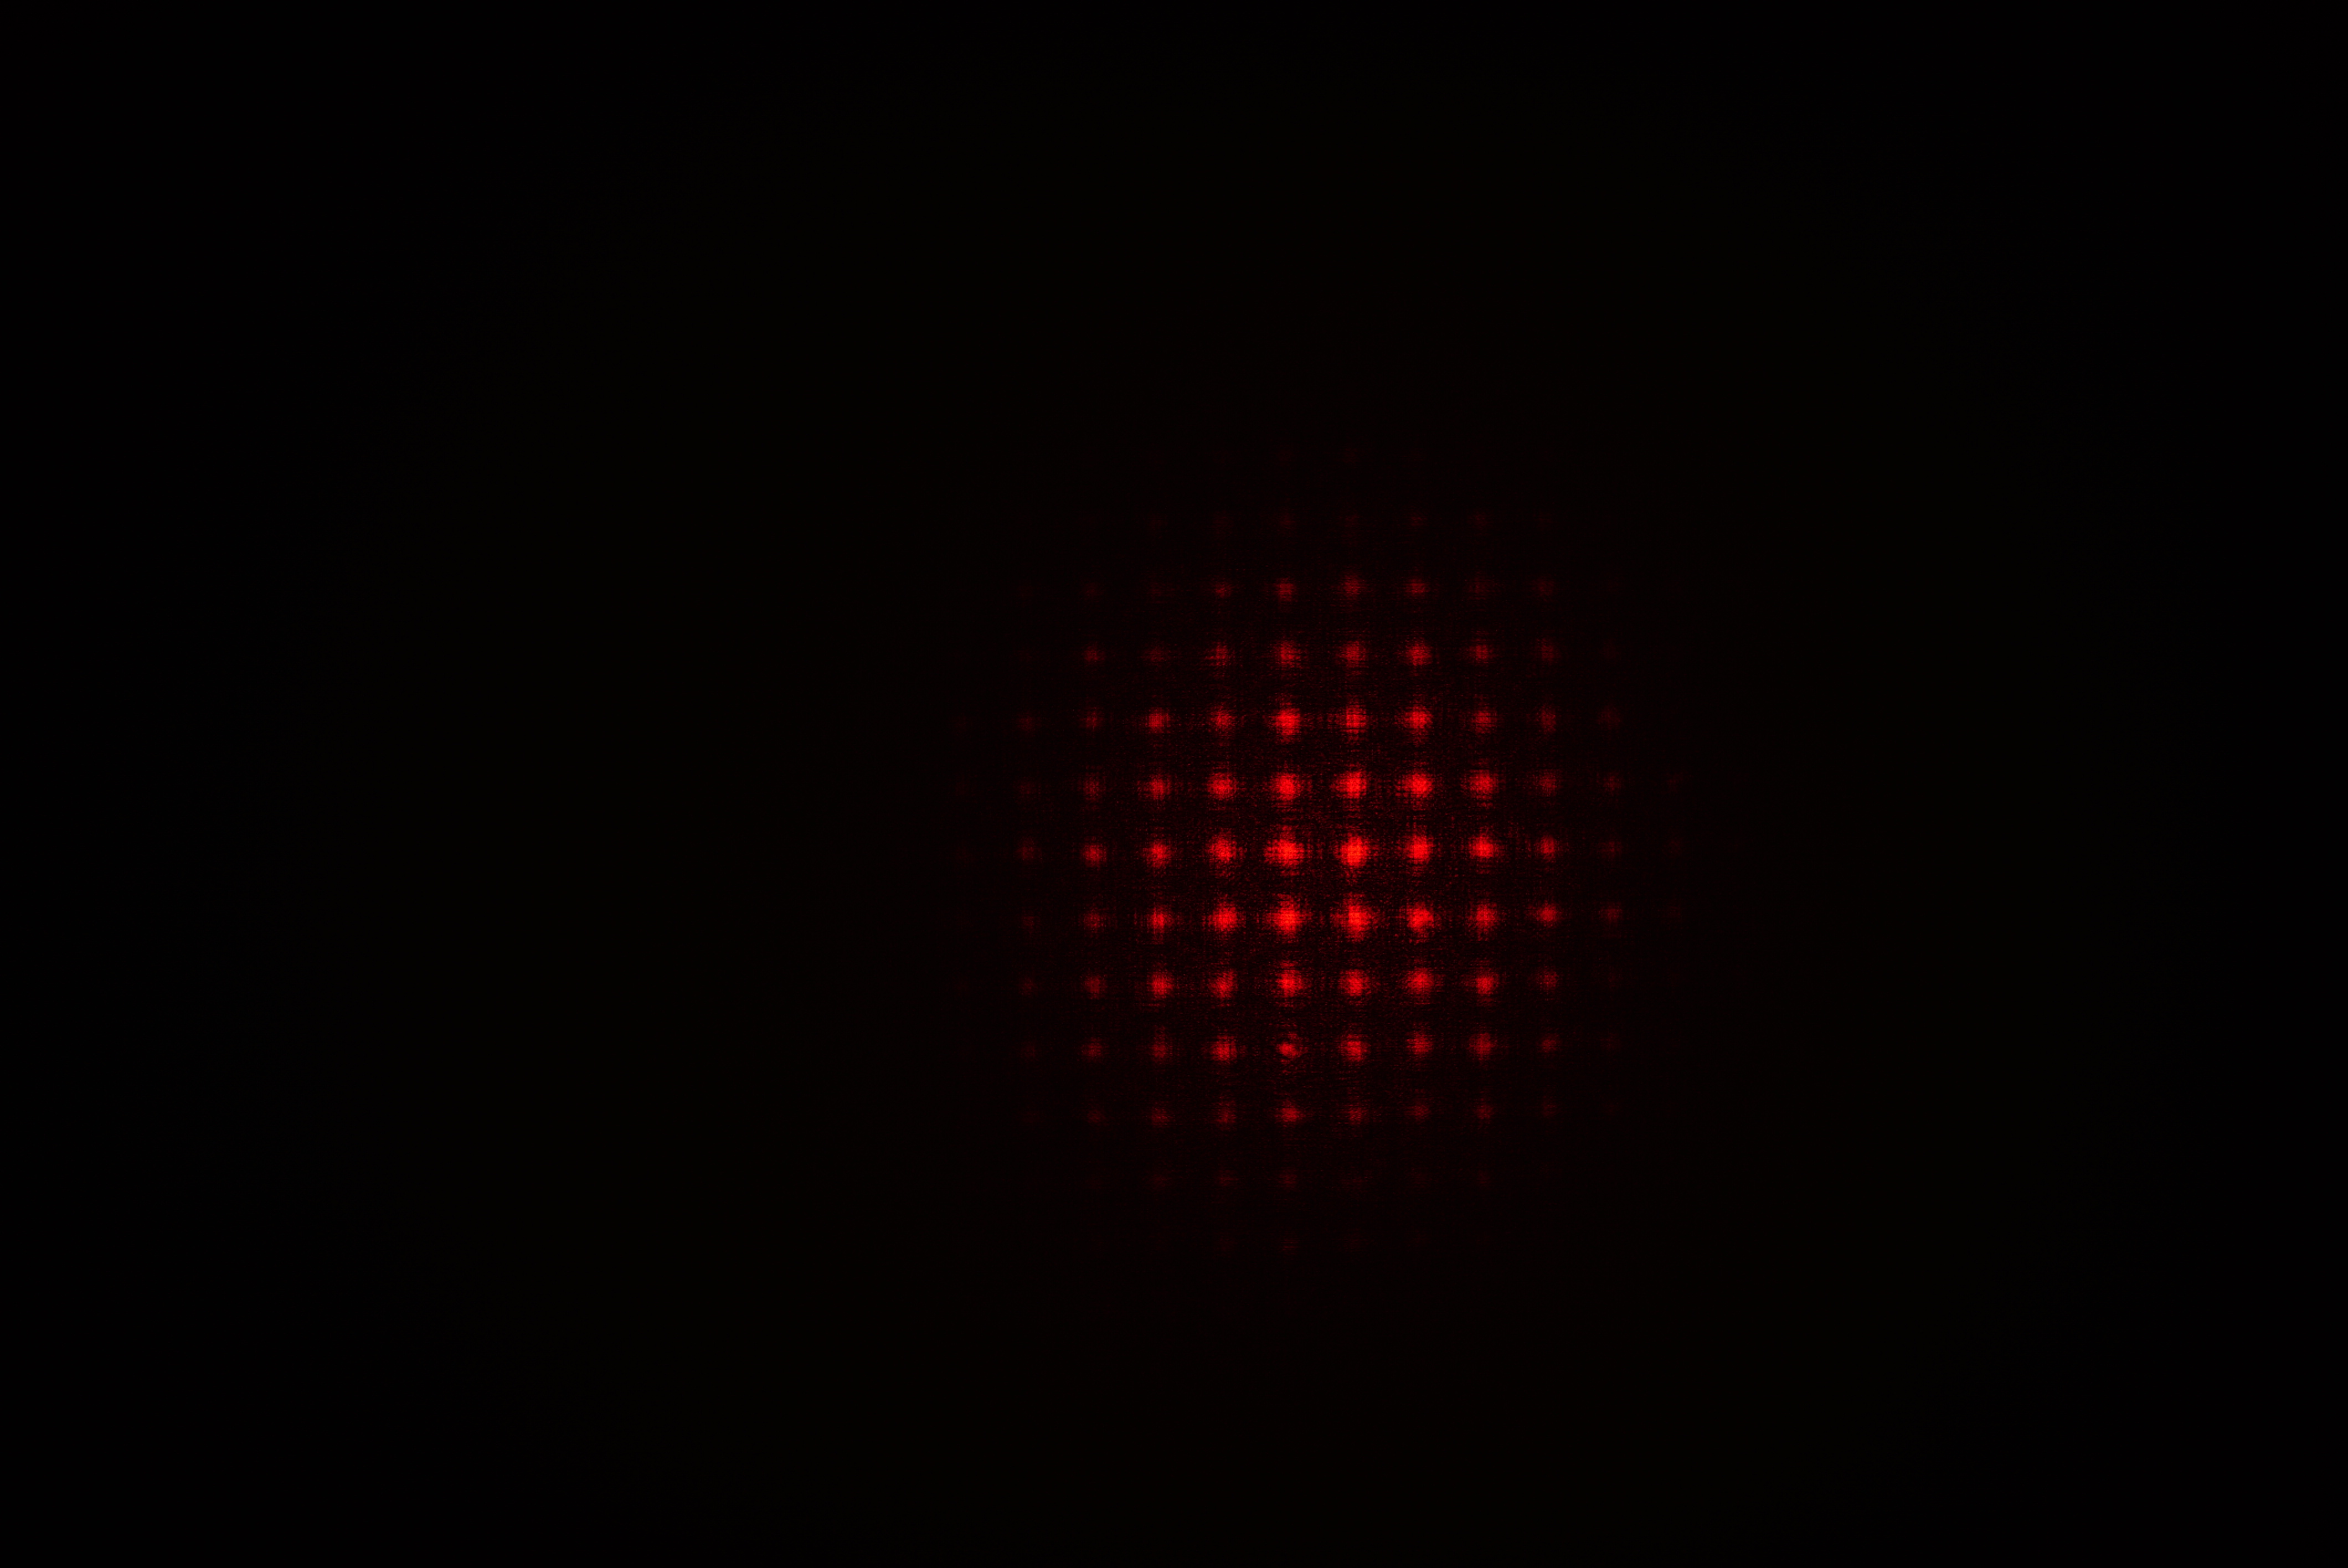
\includegraphics[ width = 0.95 \linewidth ]{figures/FilterImage/DSC01517.JPG}
        \caption{The captured image using filter 5}
    \end{minipage}%
    \begin{minipage}{0.45\textwidth}
        \centering
        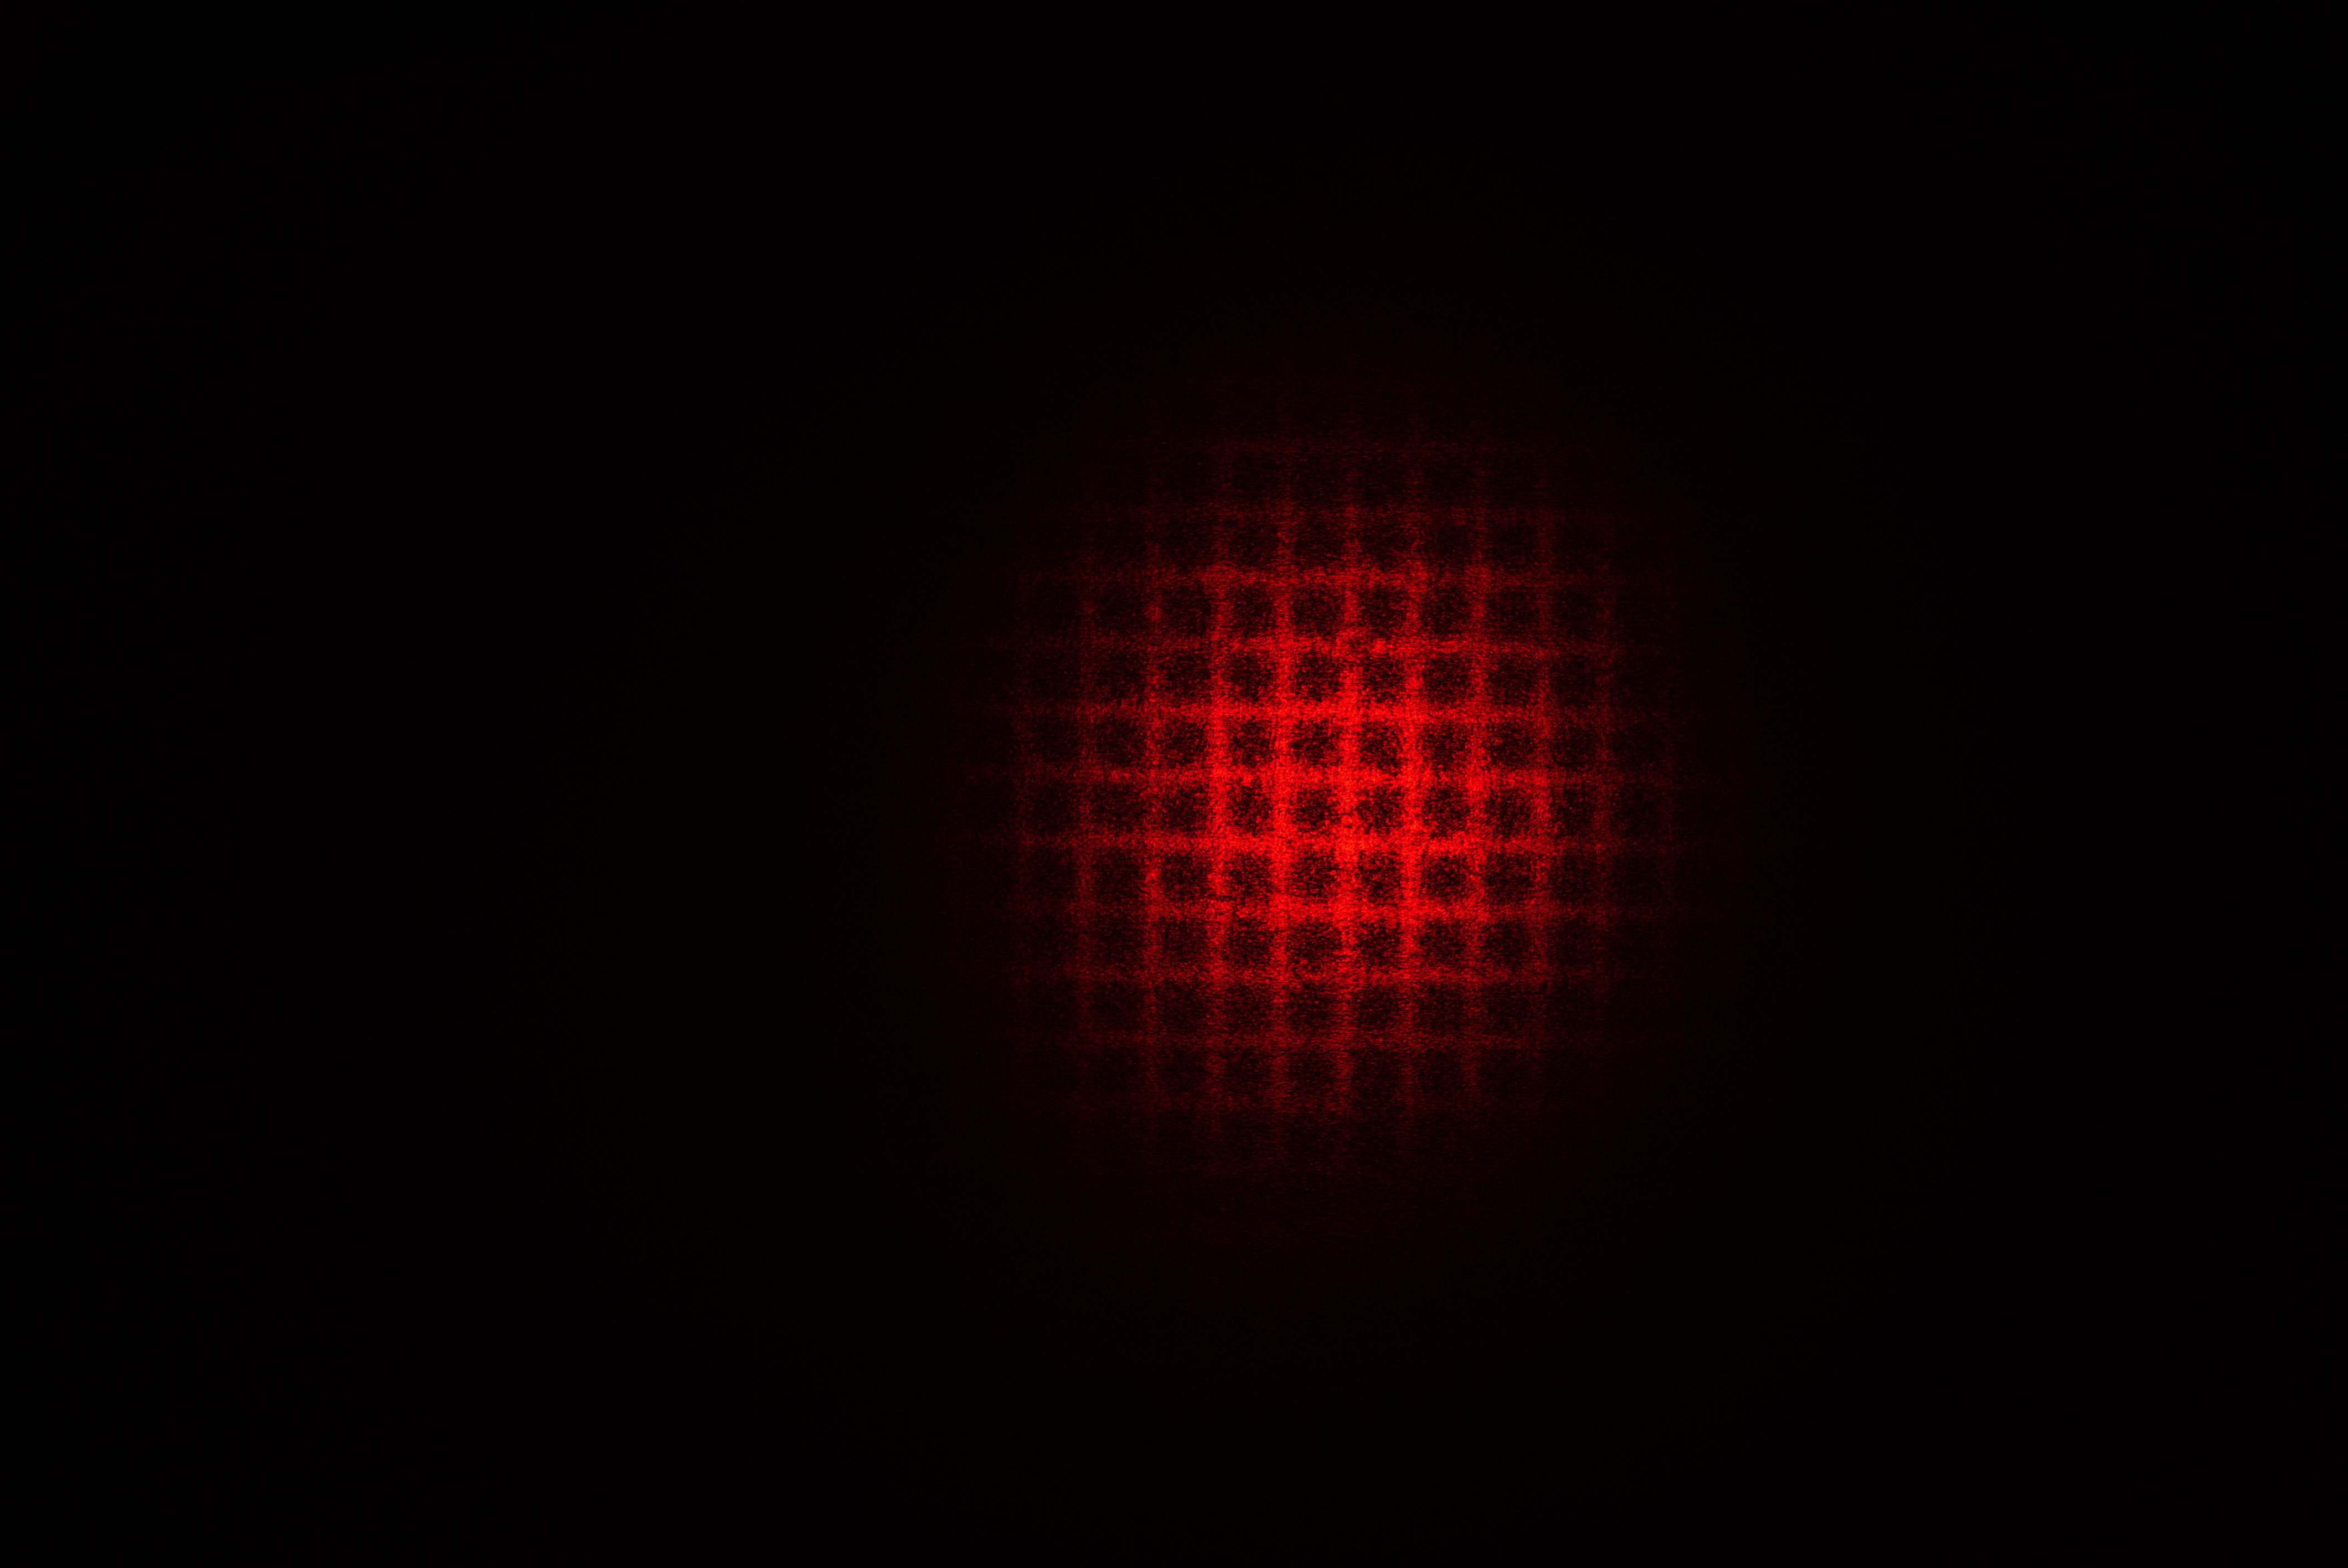
\includegraphics[ width = 0.95 \linewidth ]{figures/FilterImage/DSC01520.JPG}
        \caption{The captured image using filter 6}
    \end{minipage}%
\end{figure}

\subsection{Captured Fourier Transform}
\begin{figure}[H]
    \centering
    \begin{minipage}{0.45\textwidth}
        \centering
        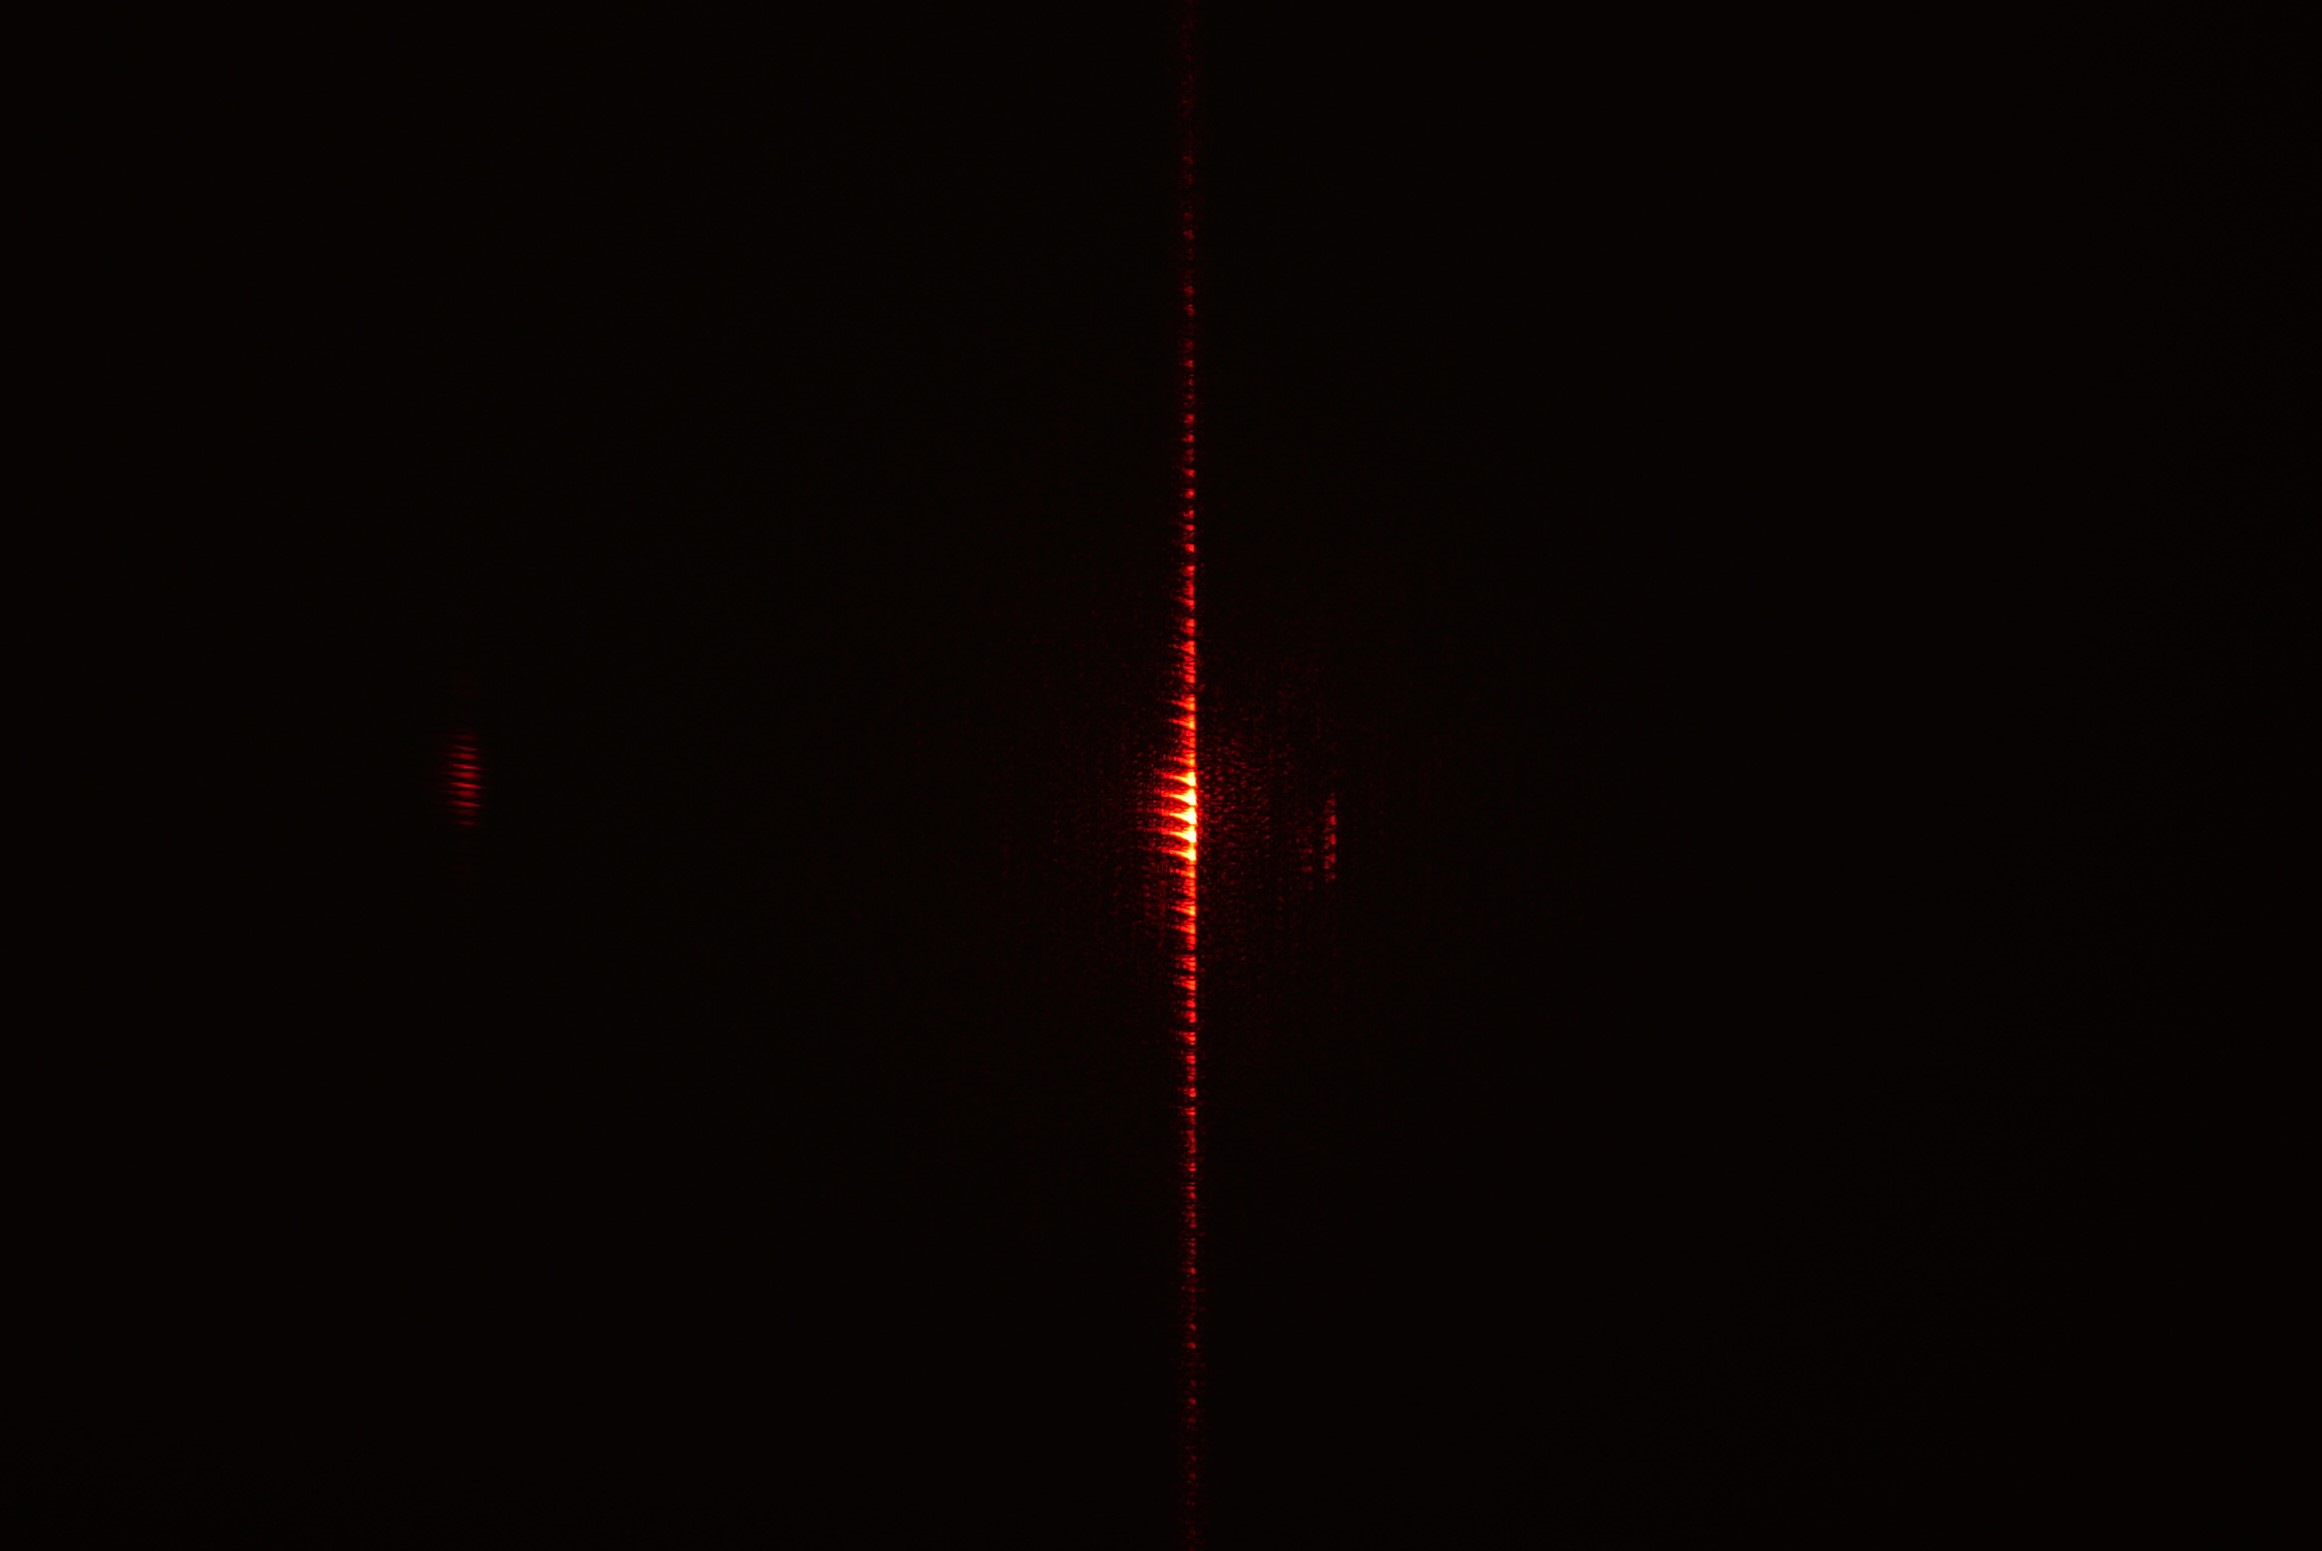
\includegraphics[ width = 0.95 \linewidth ]{figures/FT/DSC01506.JPG}
        \caption{The captured Fourier transform using filter 1}
    \end{minipage}%
    \begin{minipage}{0.45\textwidth}
        \centering
        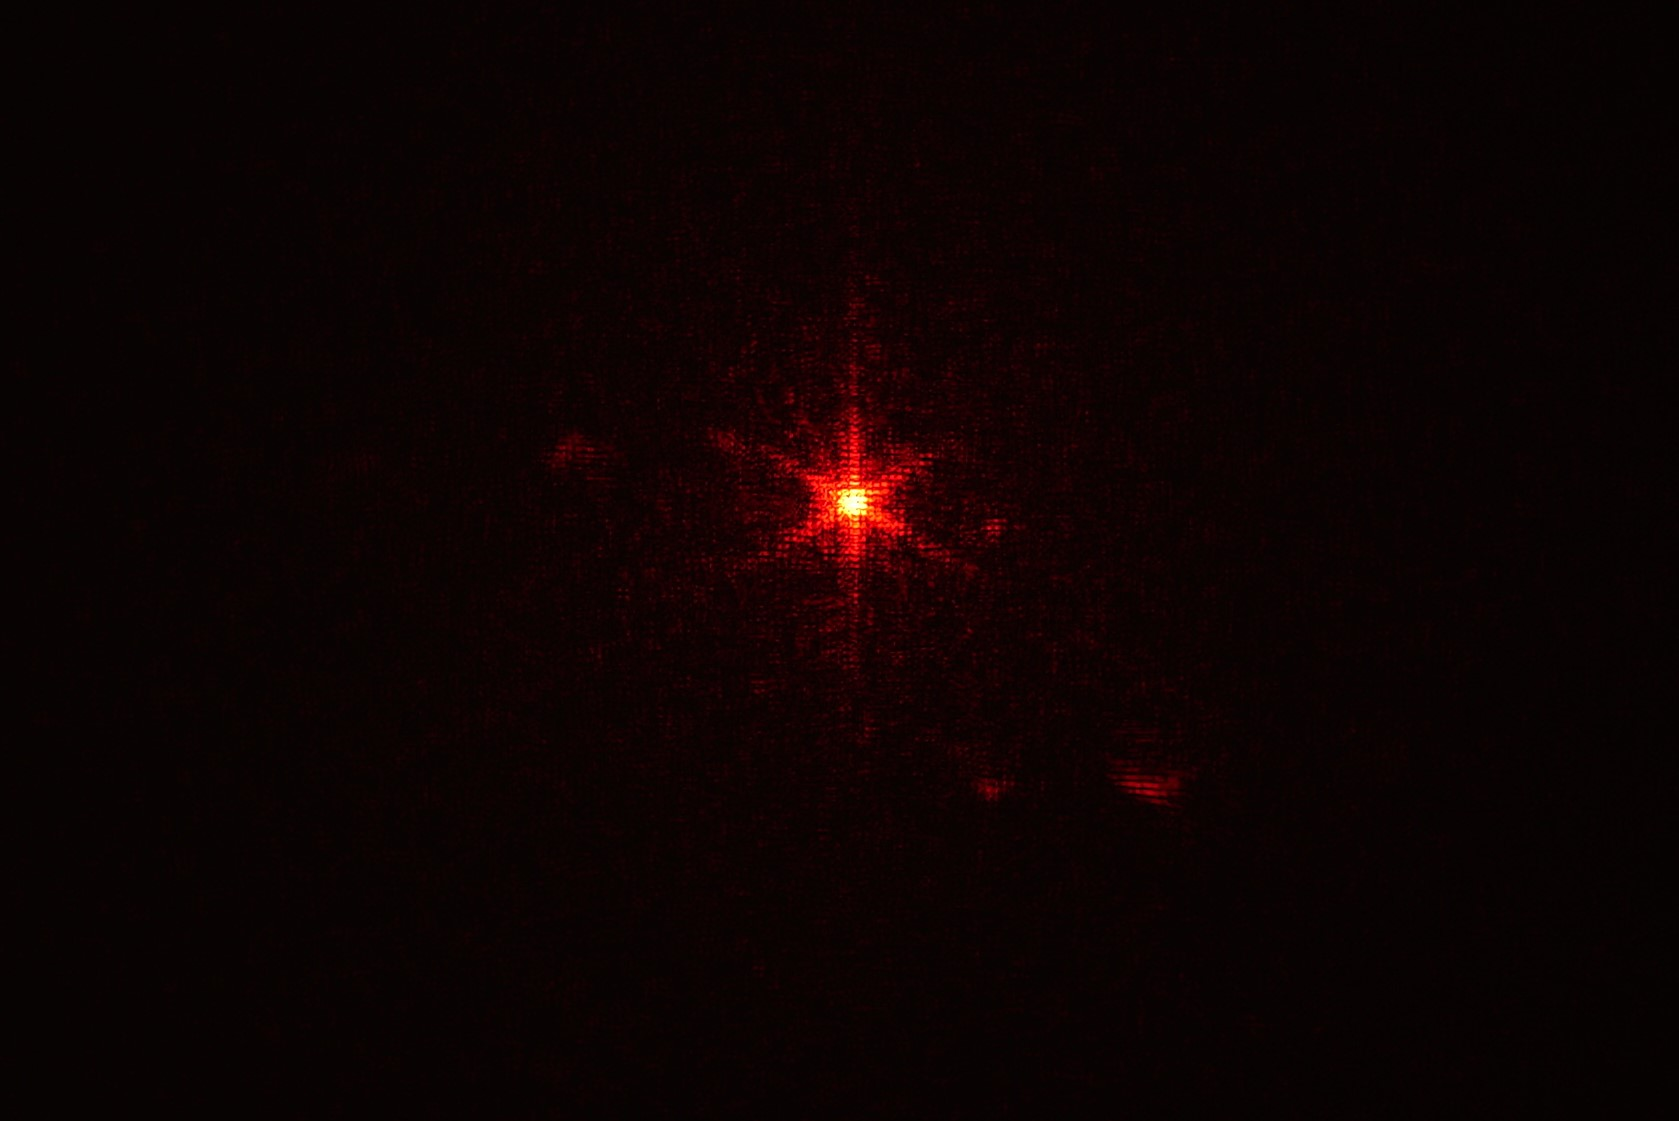
\includegraphics[ width = 0.95 \linewidth ]{figures/FT/DSC01509.JPG}
        \caption{The captured Fourier transform using filter 2}
    \end{minipage}%
    \vspace{2cm}
    \begin{minipage}{0.45\textwidth}
        \centering
        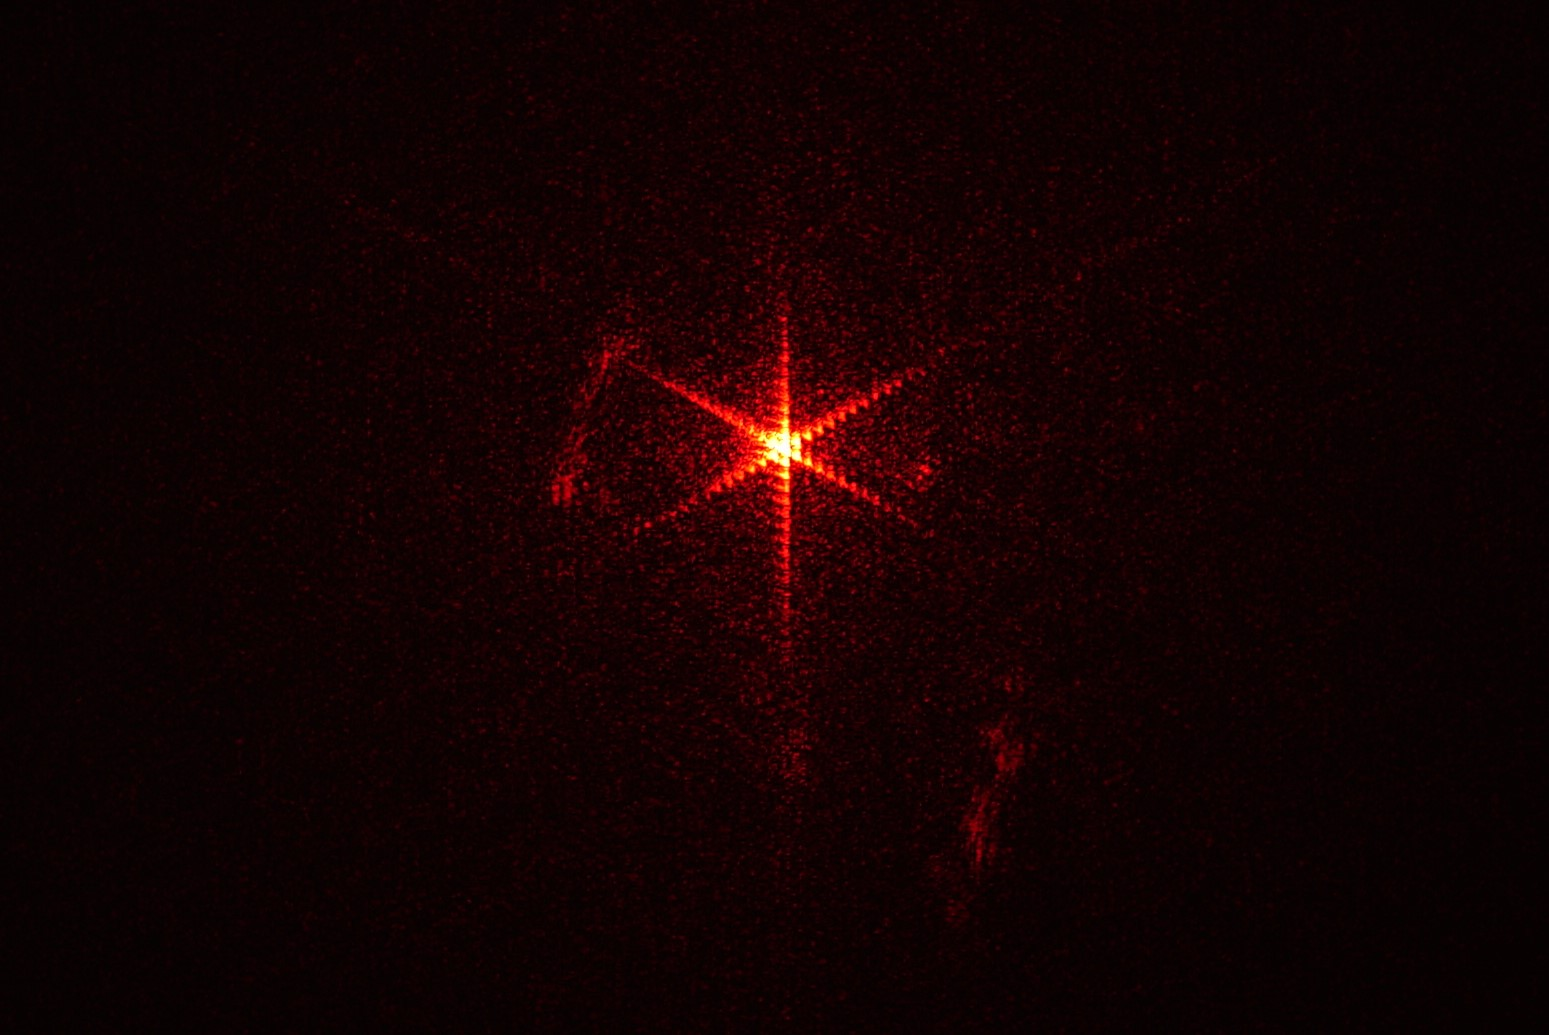
\includegraphics[ width = 0.95 \linewidth ]{figures/FT/DSC01512.JPG}
        \caption{The captured Fourier transform using filter 3}
    \end{minipage}%
    \begin{minipage}{0.45\textwidth}
        \centering
        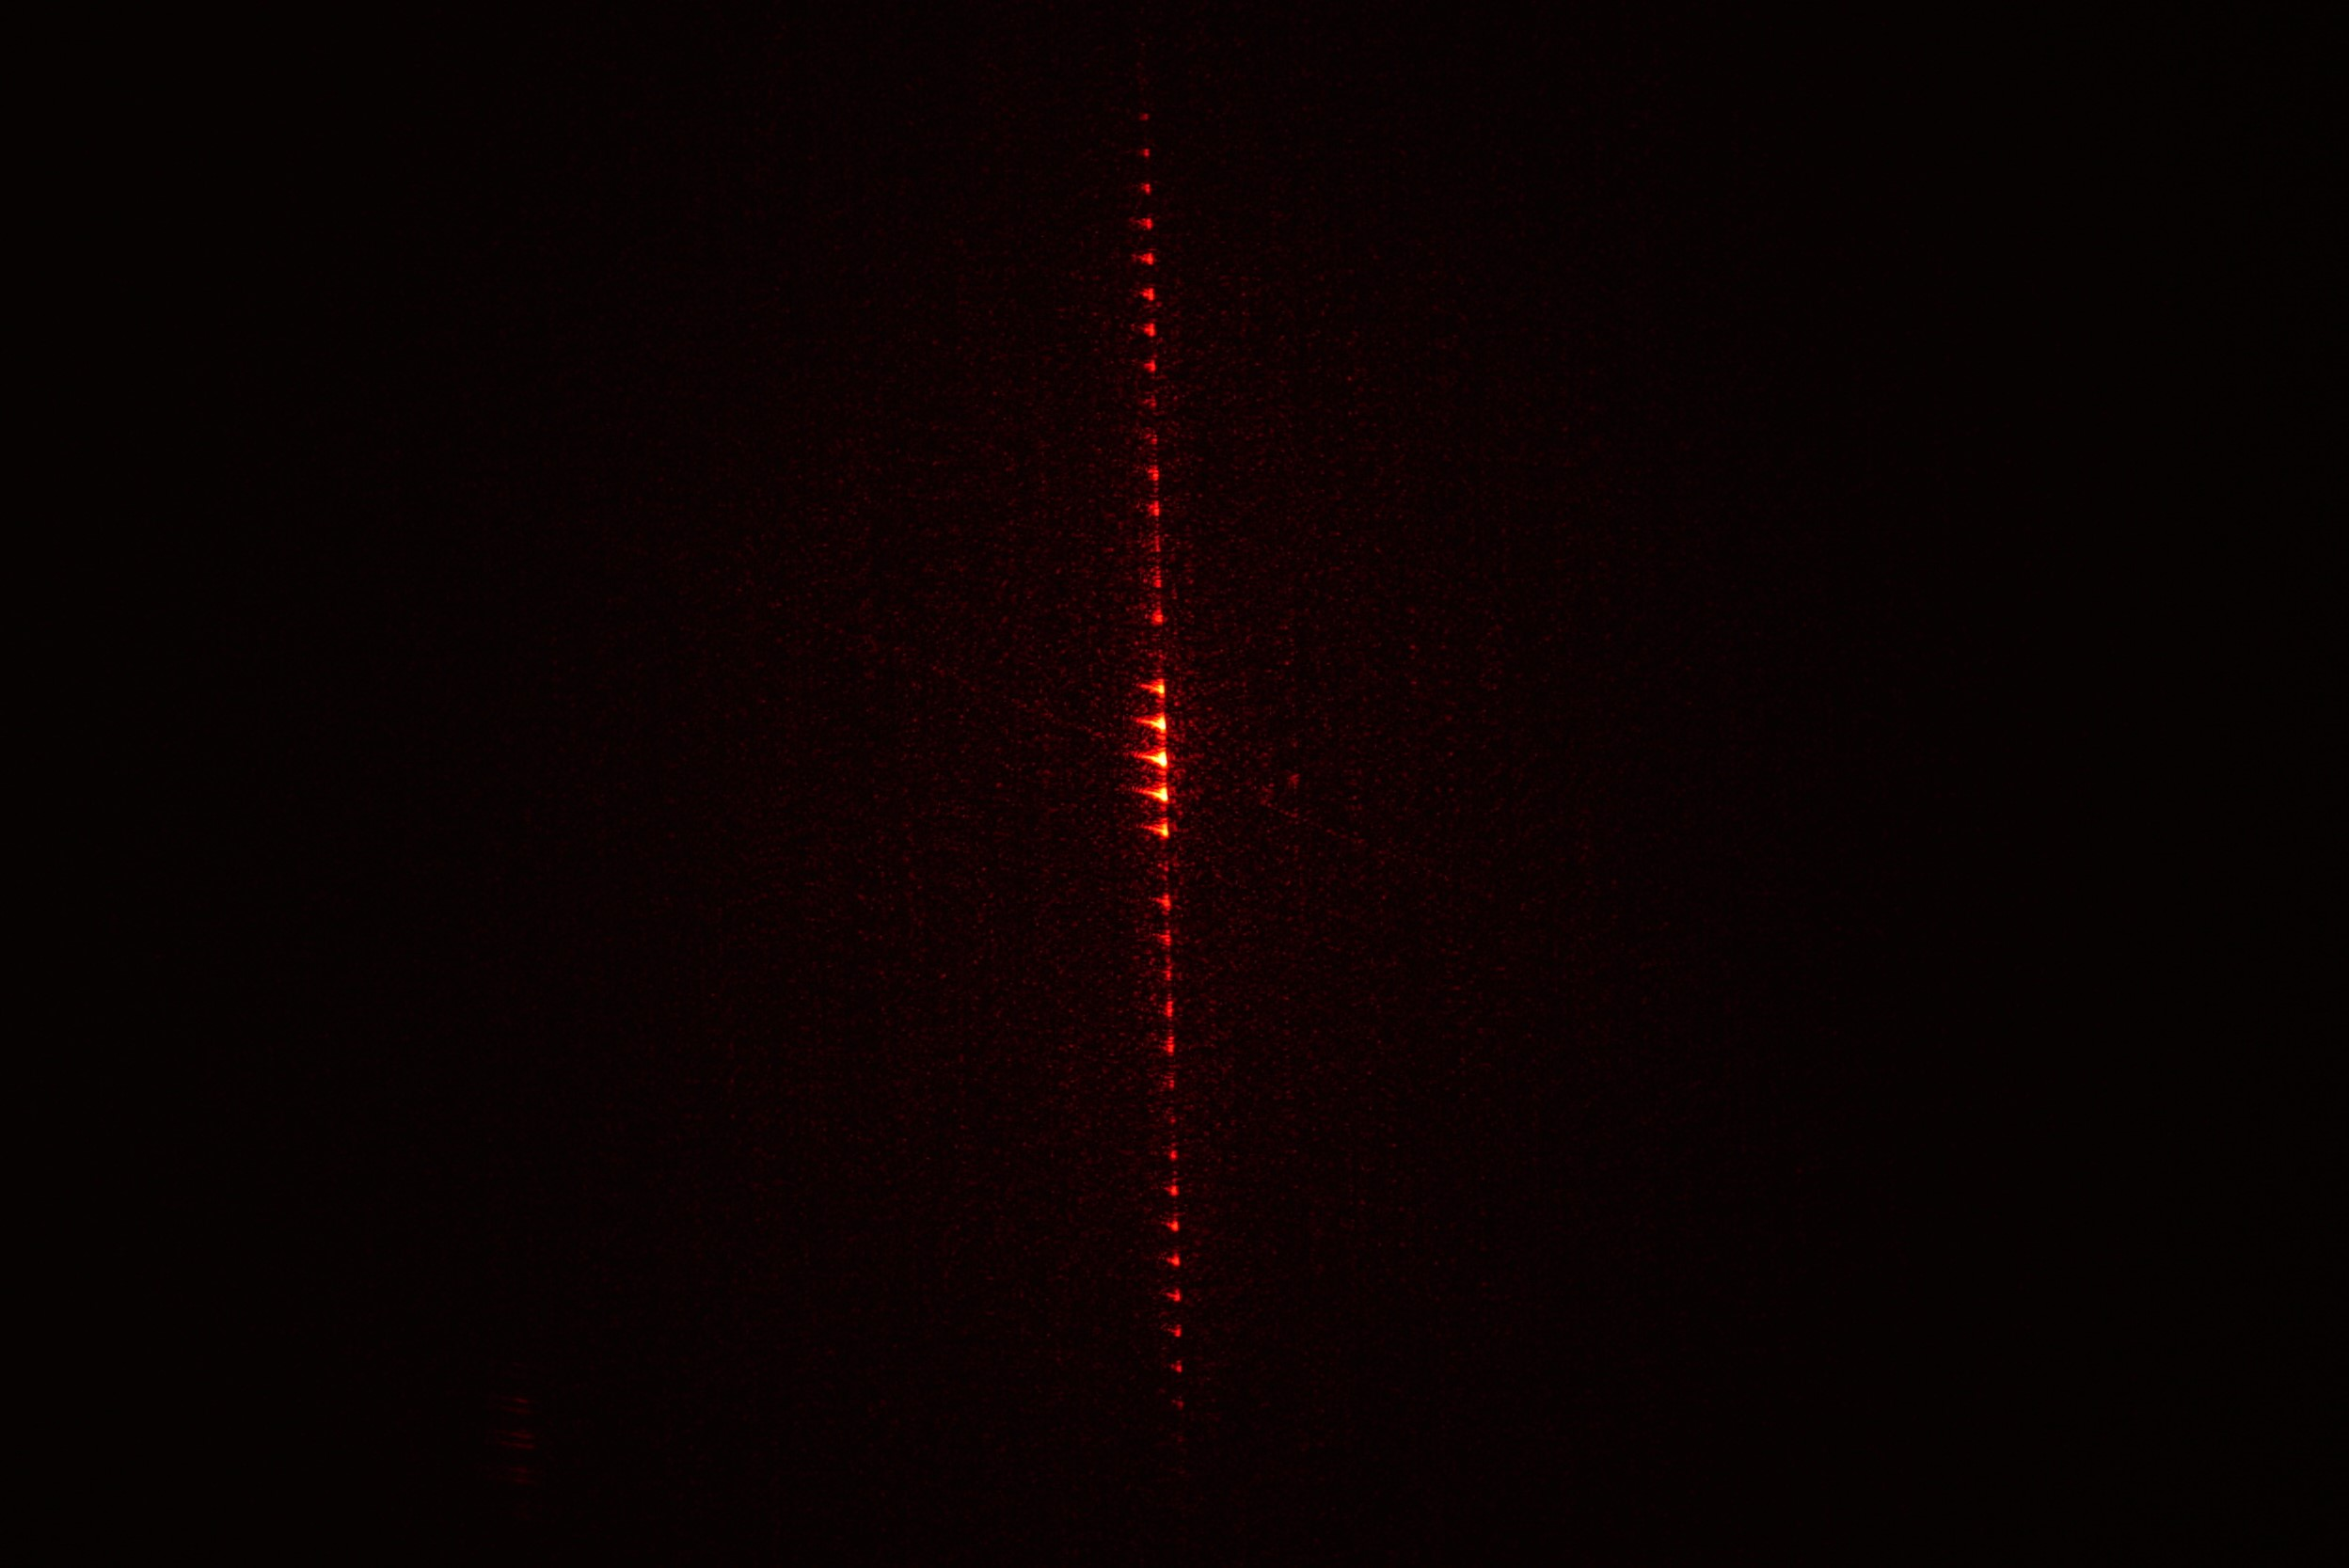
\includegraphics[ width = 0.95 \linewidth ]{figures/FT/DSC01515.JPG}
        \caption{The captured Fourier transform using filter 4}
    \end{minipage}%
    \vspace{2cm}
    \begin{minipage}{0.45\textwidth}
        \centering
        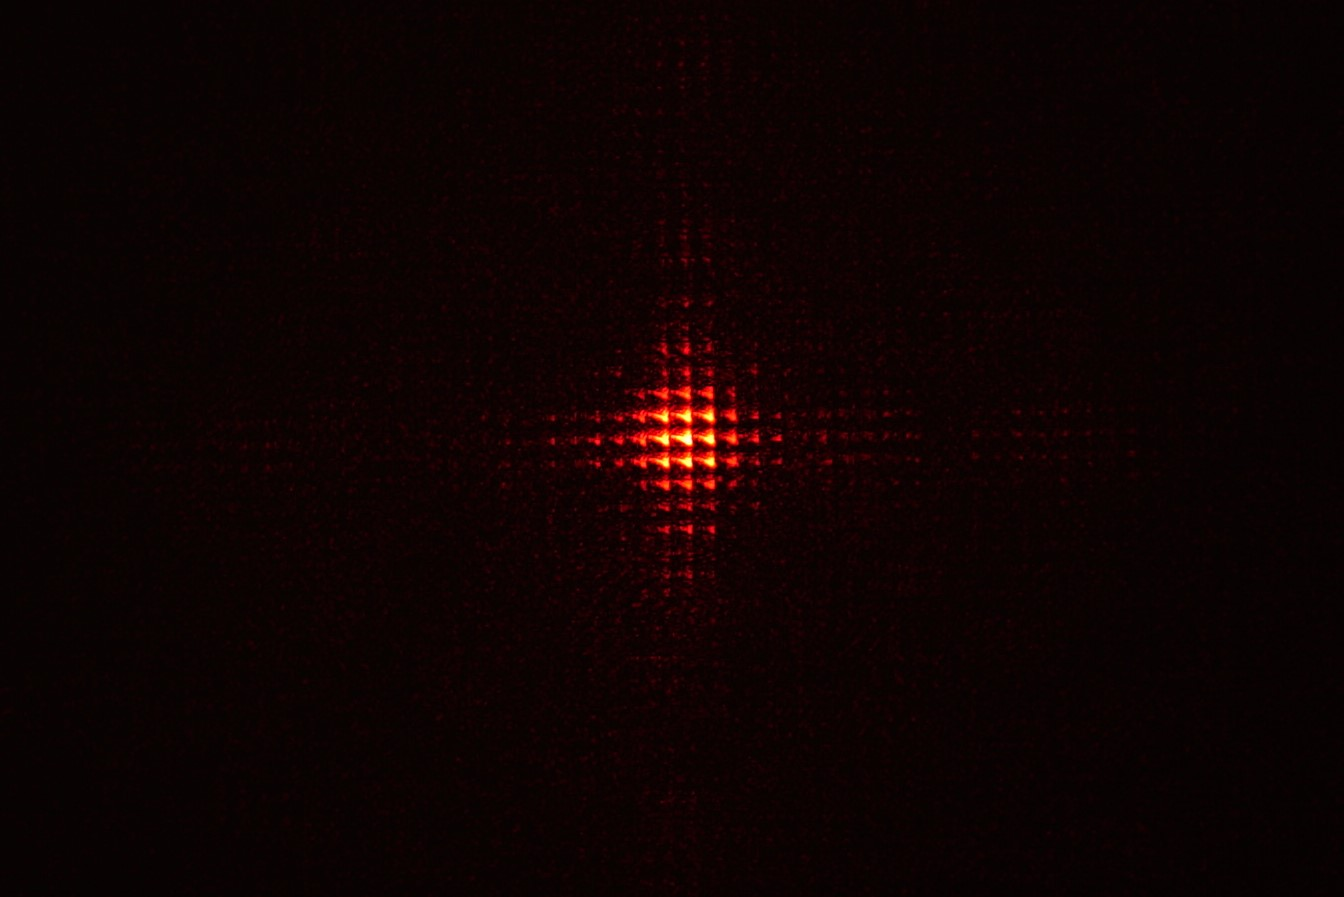
\includegraphics[ width = 0.95 \linewidth ]{figures/FT/DSC01518.JPG}
        \caption{The captured Fourier transform using filter 5}
    \end{minipage}%
    \begin{minipage}{0.45\textwidth}
        \centering
        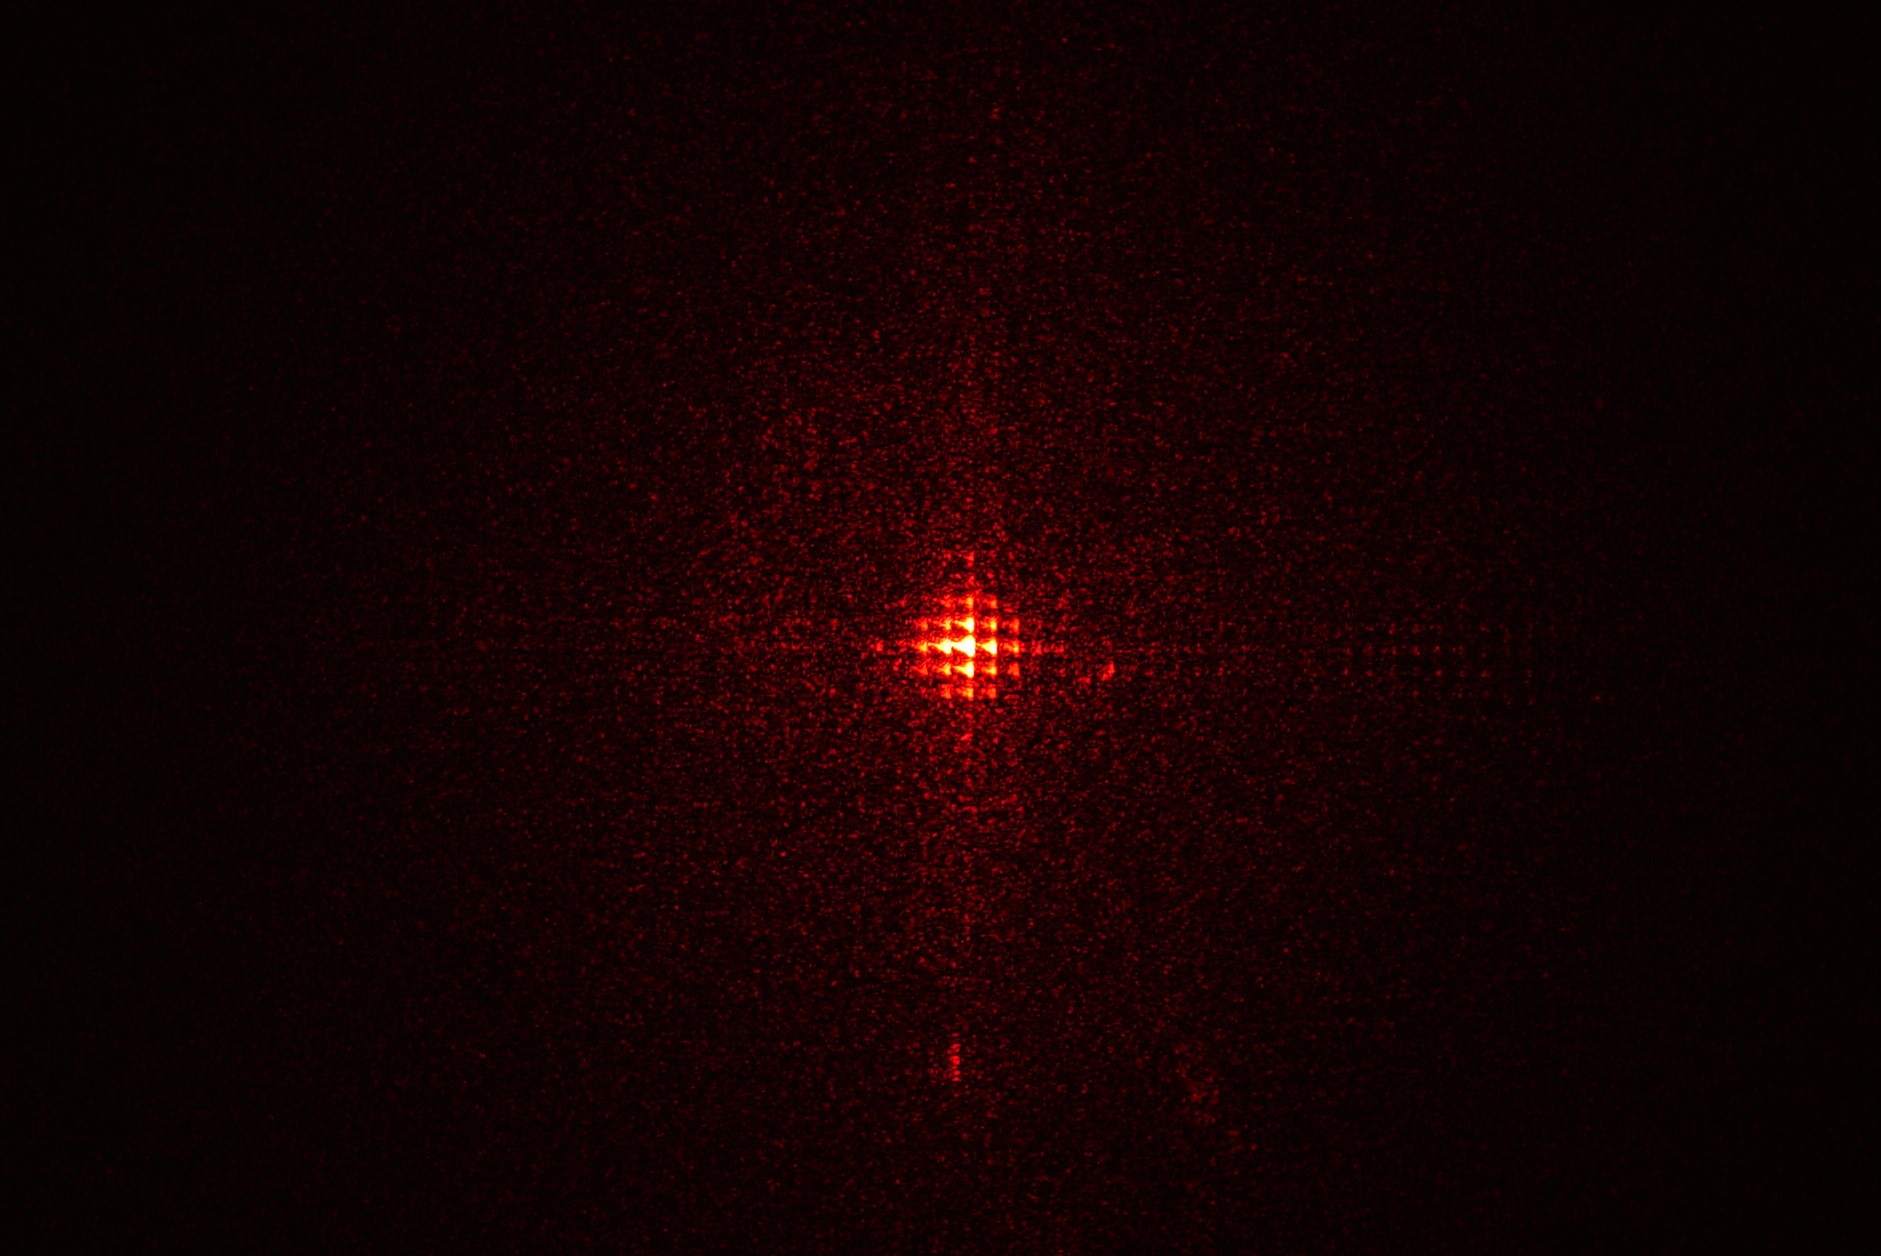
\includegraphics[ width = 0.95 \linewidth ]{figures/FT/DSC01521.JPG}
        \caption{The captured Fourier transform using filter 6}
    \end{minipage}%
\end{figure}

\subsection{Captured Inverse Fourier Transform}
\begin{figure}[H]
    \centering
    \begin{minipage}{0.45\textwidth}
        \centering
        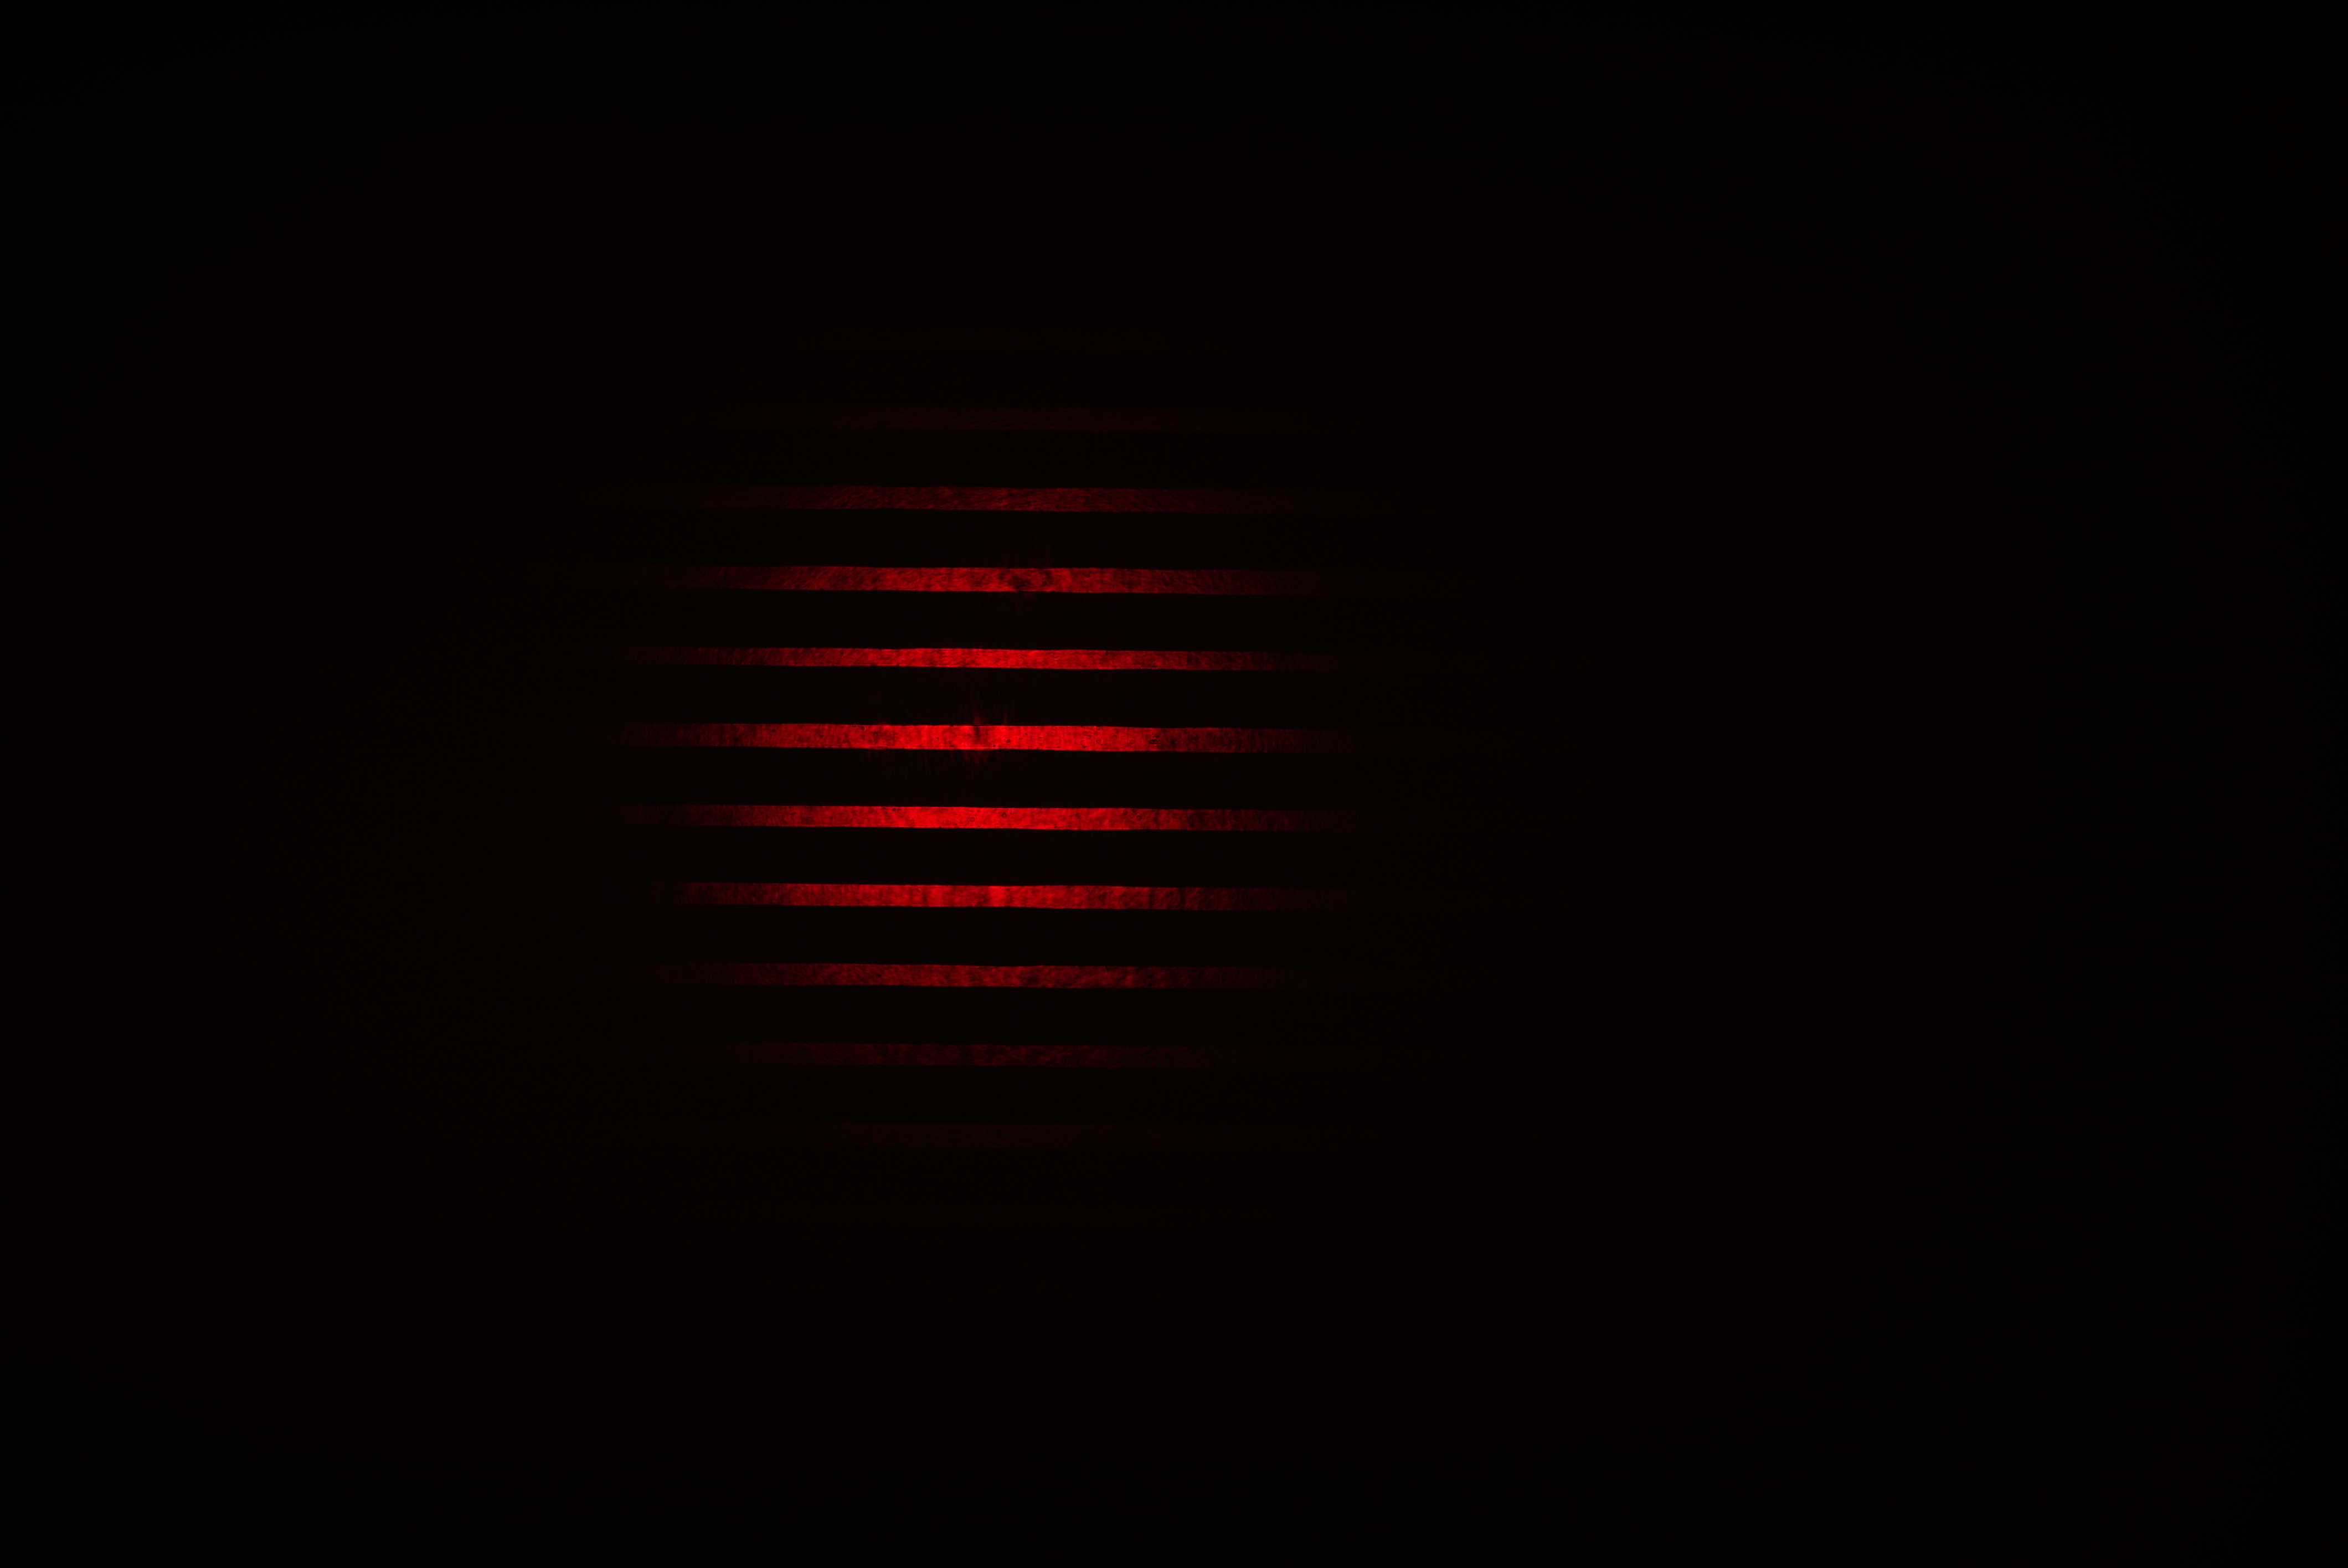
\includegraphics[ width = 0.95 \linewidth ]{figures/Inverse FT/DSC01507.JPG}
        \caption{The captured inverse FT using filter 1}
    \end{minipage}%
    \begin{minipage}{0.45\textwidth}
        \centering
        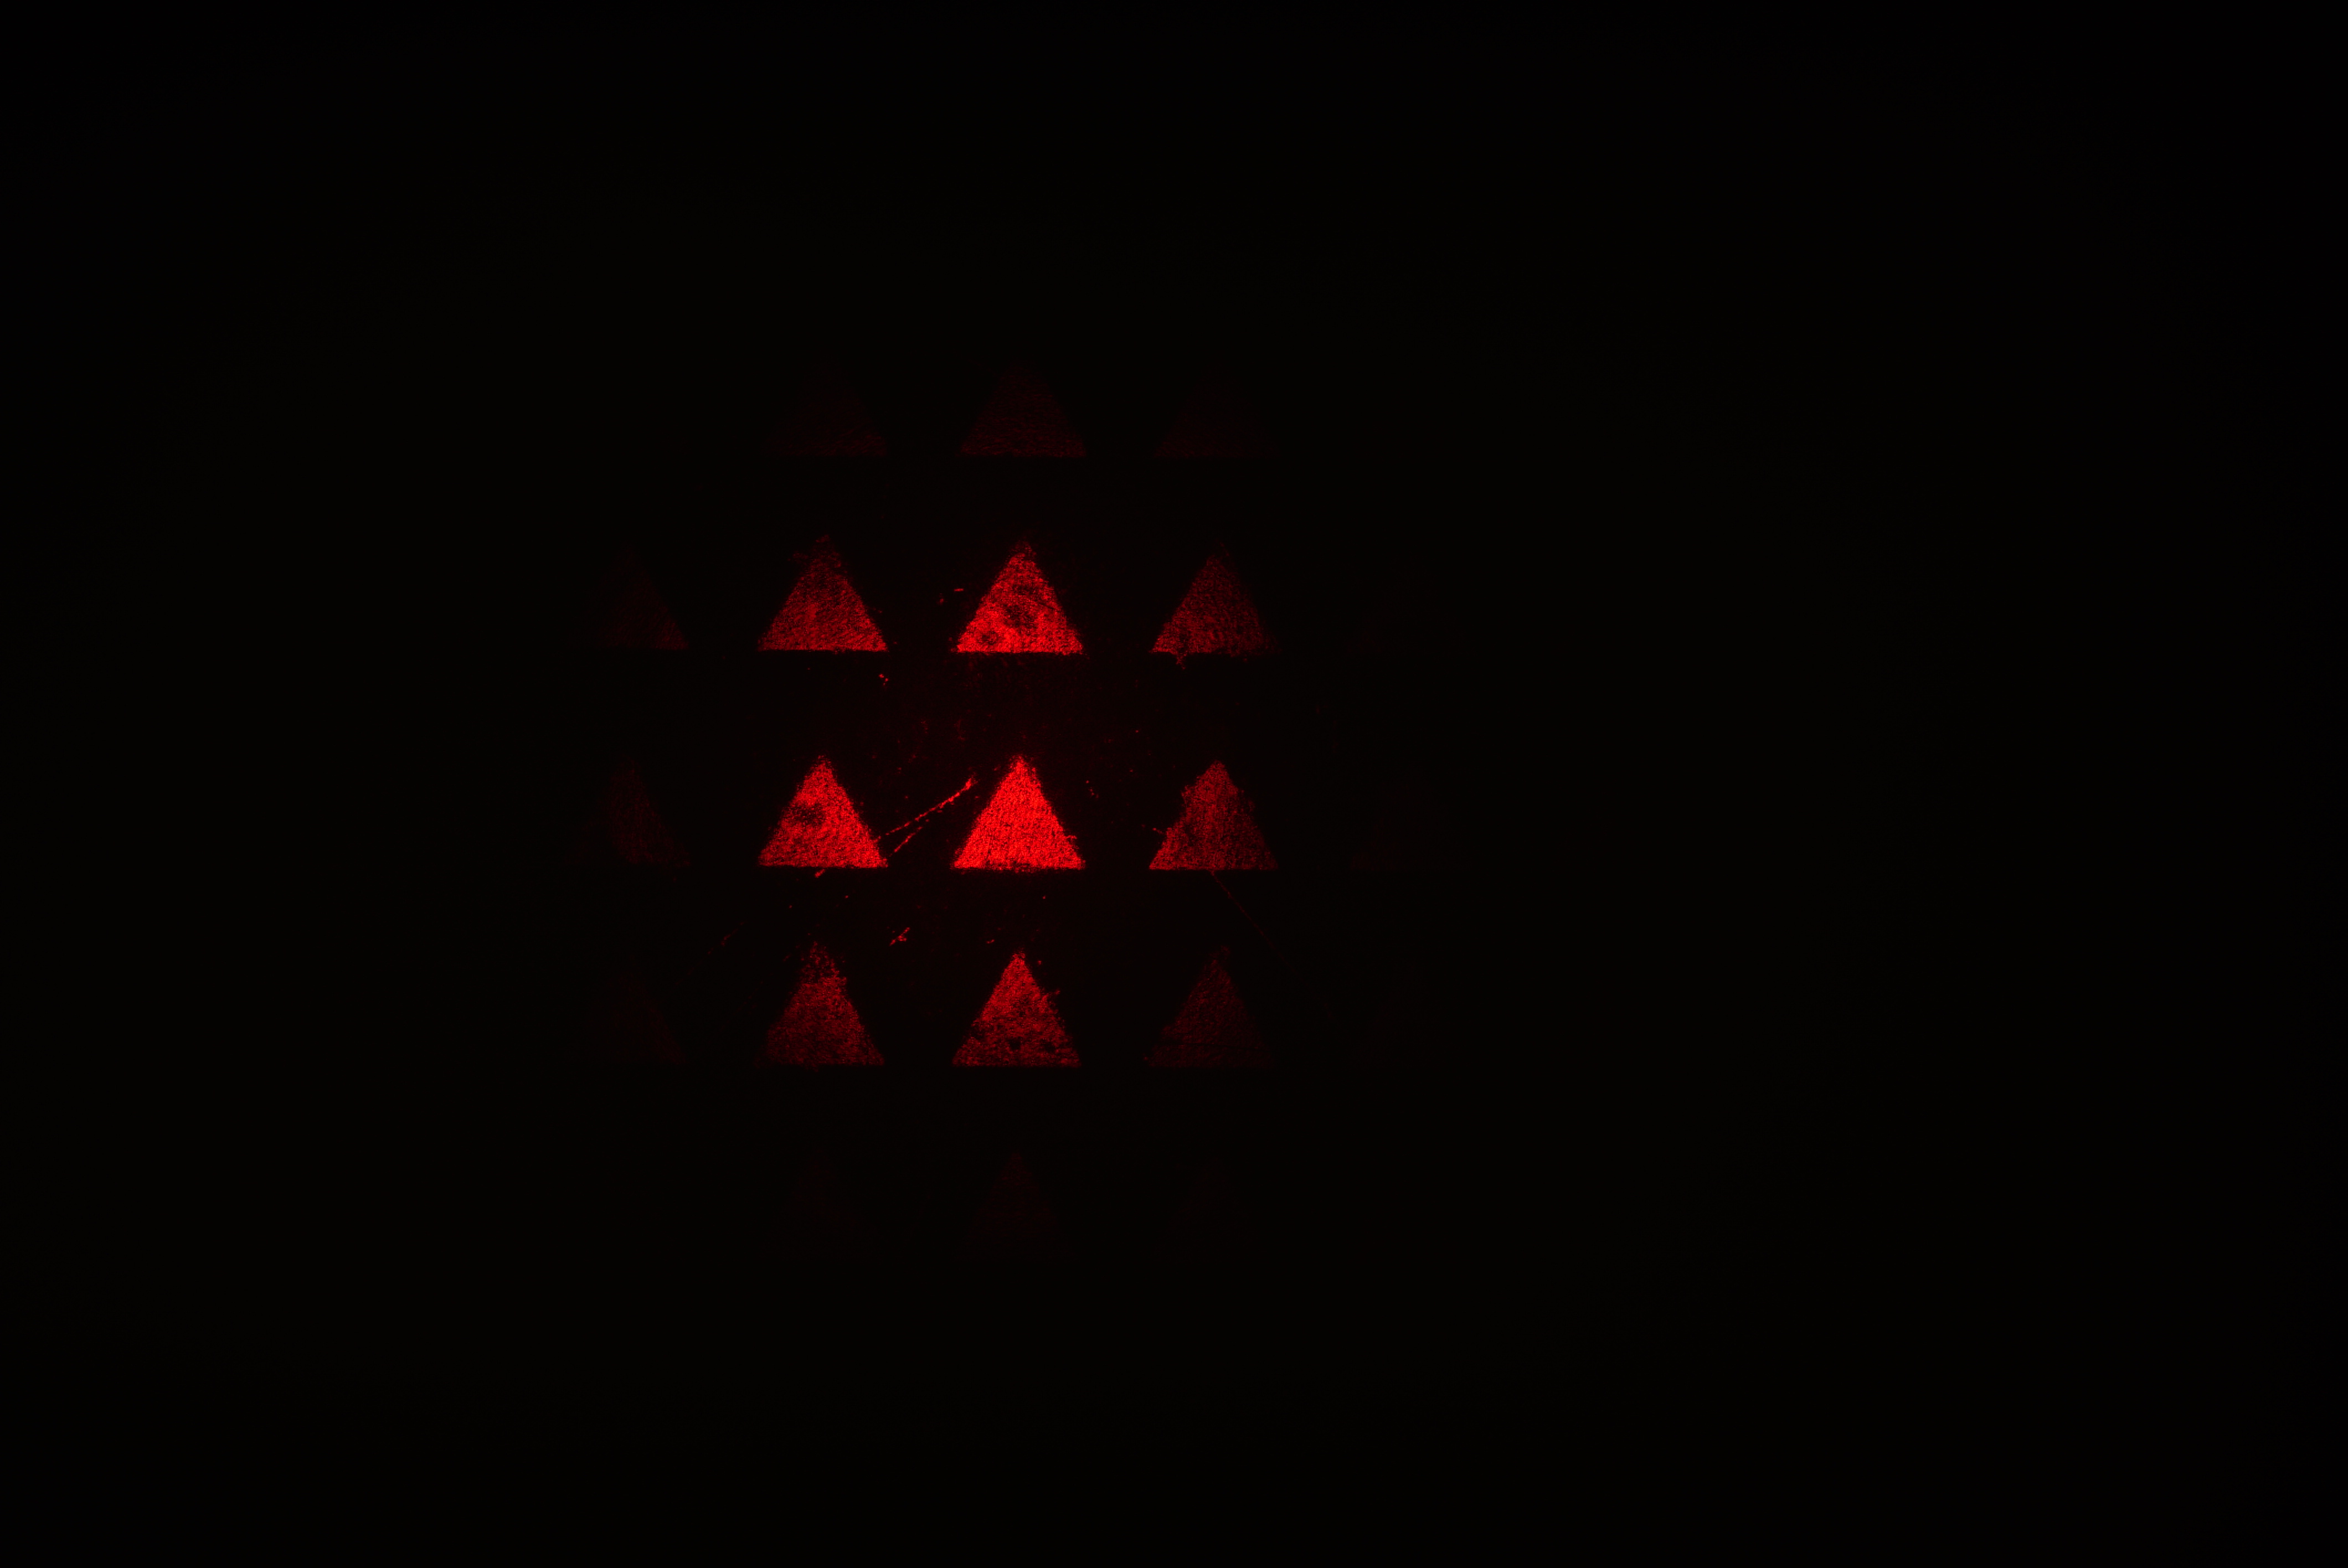
\includegraphics[ width = 0.95 \linewidth ]{figures/Inverse FT/DSC01510.JPG}
        \caption{The captured inverse FT using filter 2}
    \end{minipage}%
    \vspace{2cm}
    \begin{minipage}{0.45\textwidth}
        \centering
        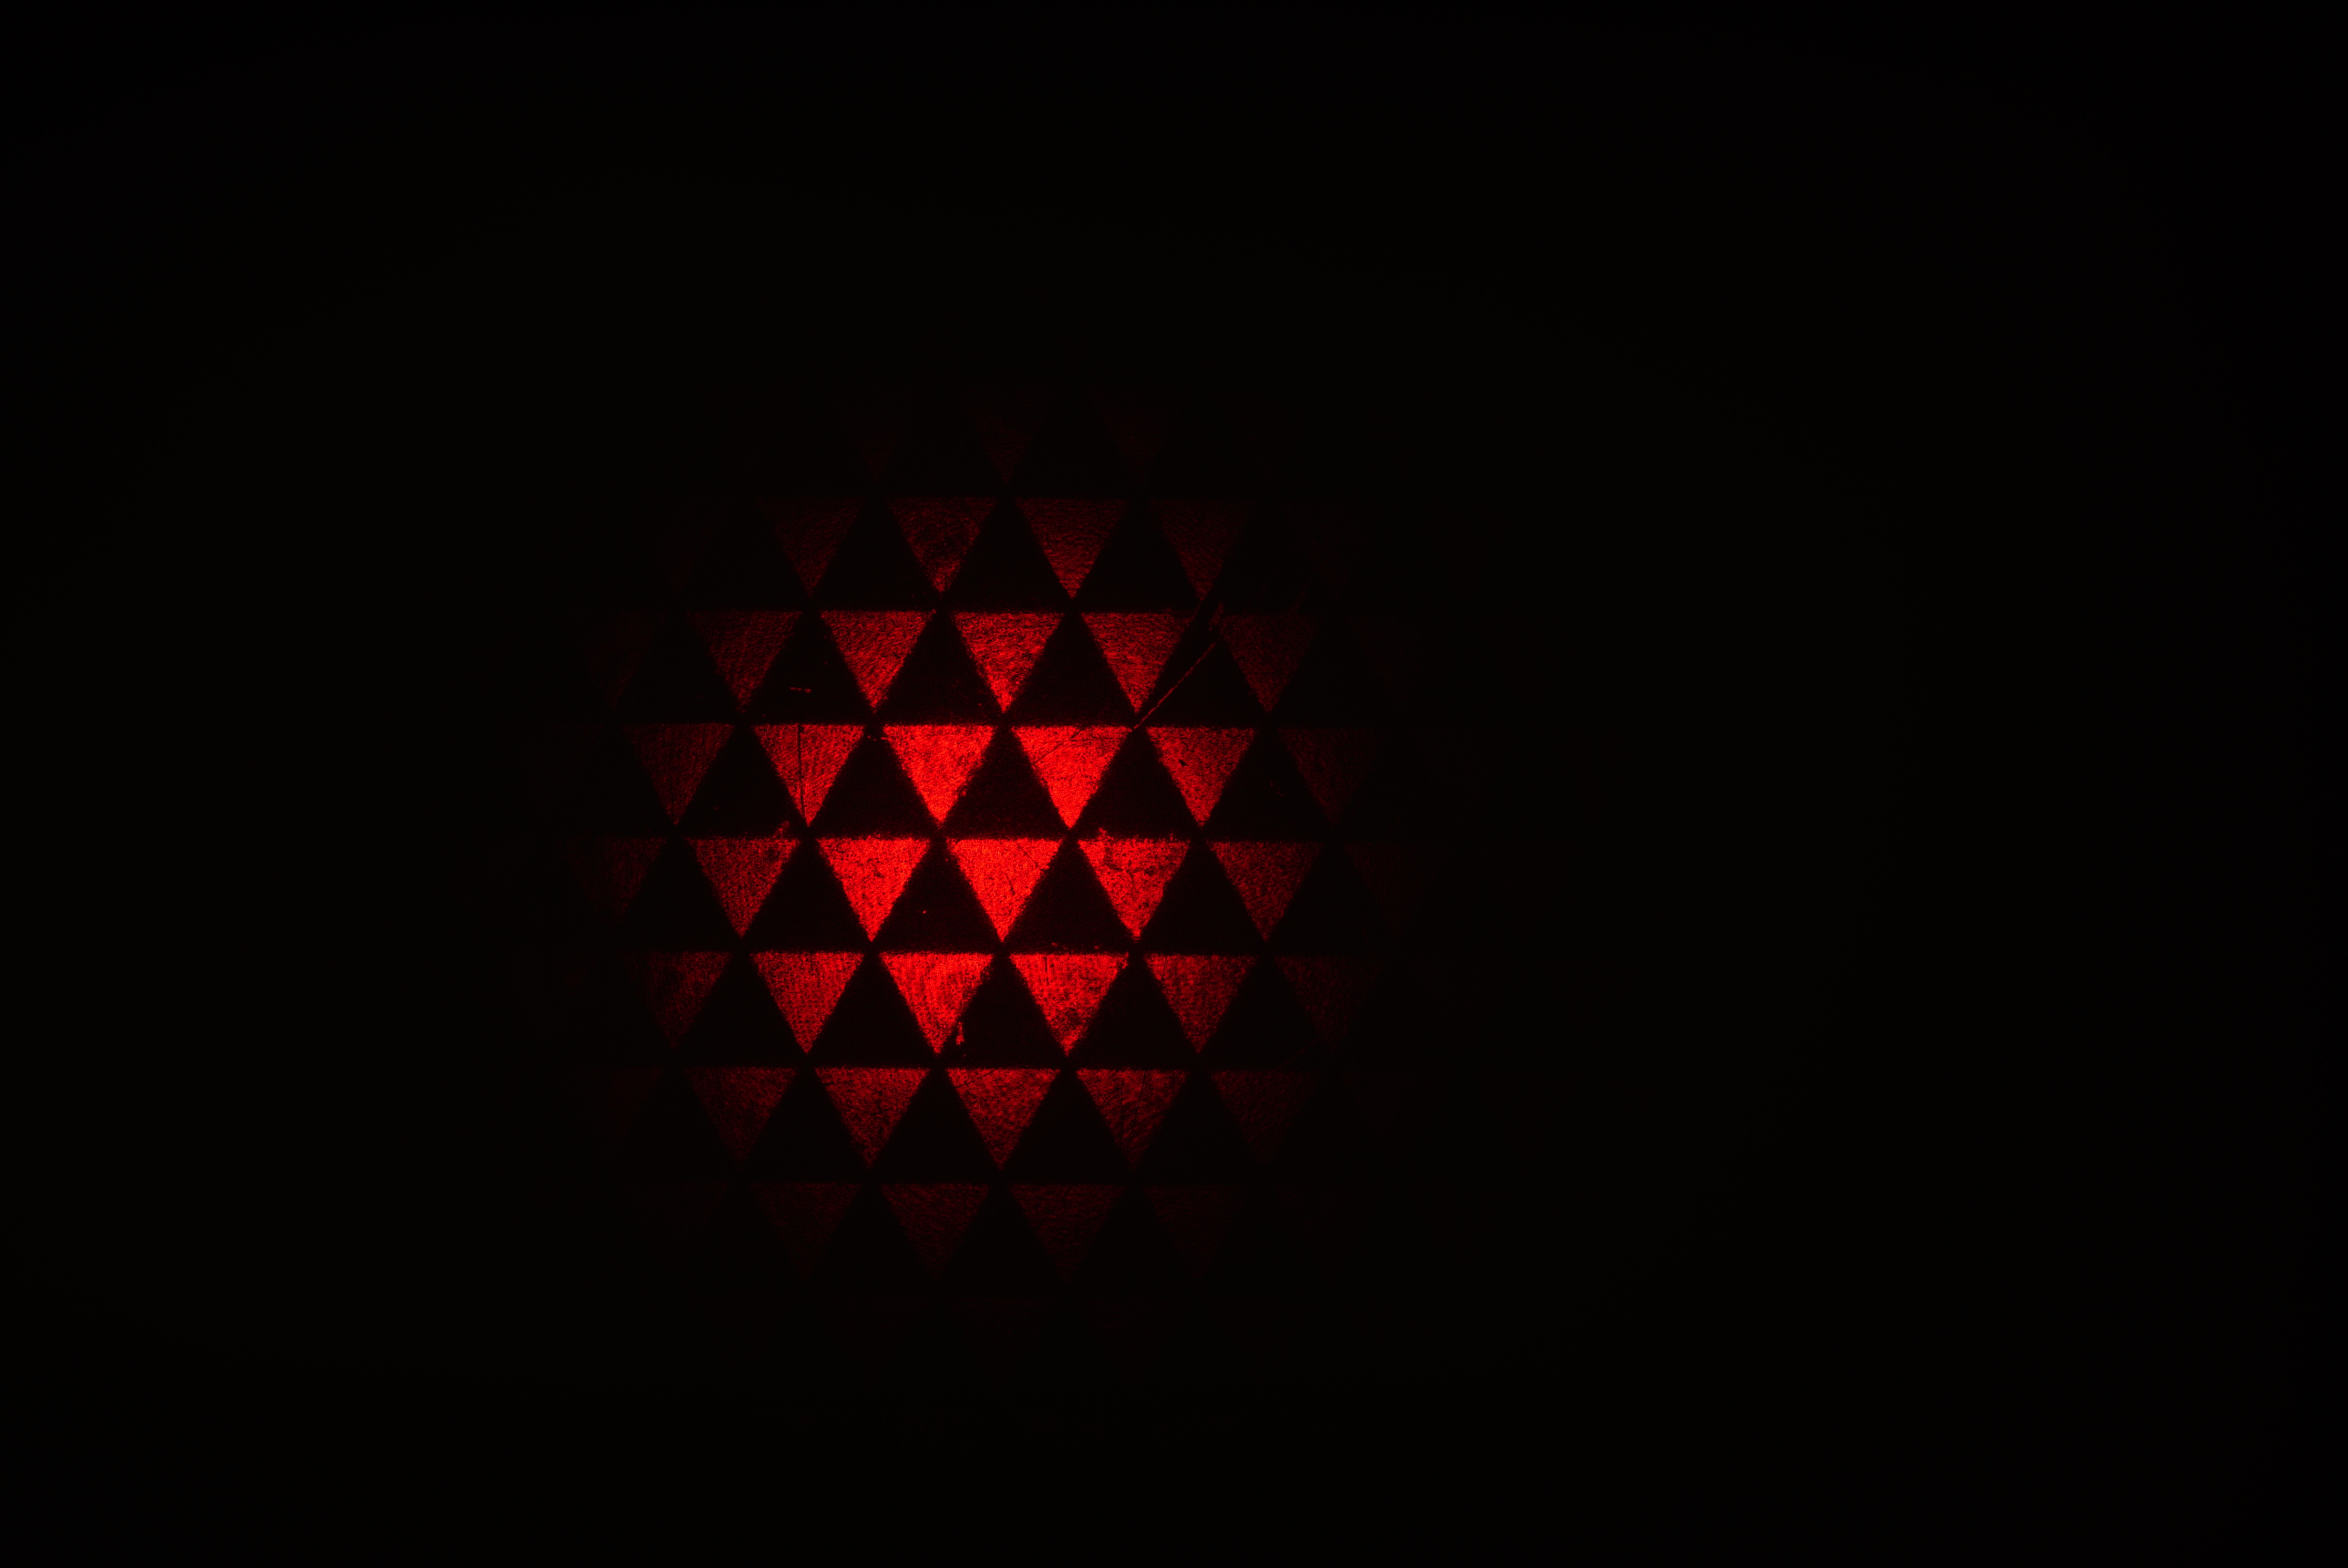
\includegraphics[ width = 0.95 \linewidth ]{figures/Inverse FT/DSC01513.JPG}
        \caption{The captured inverse FT using filter 3}
    \end{minipage}%
    \begin{minipage}{0.45\textwidth}
        \centering
        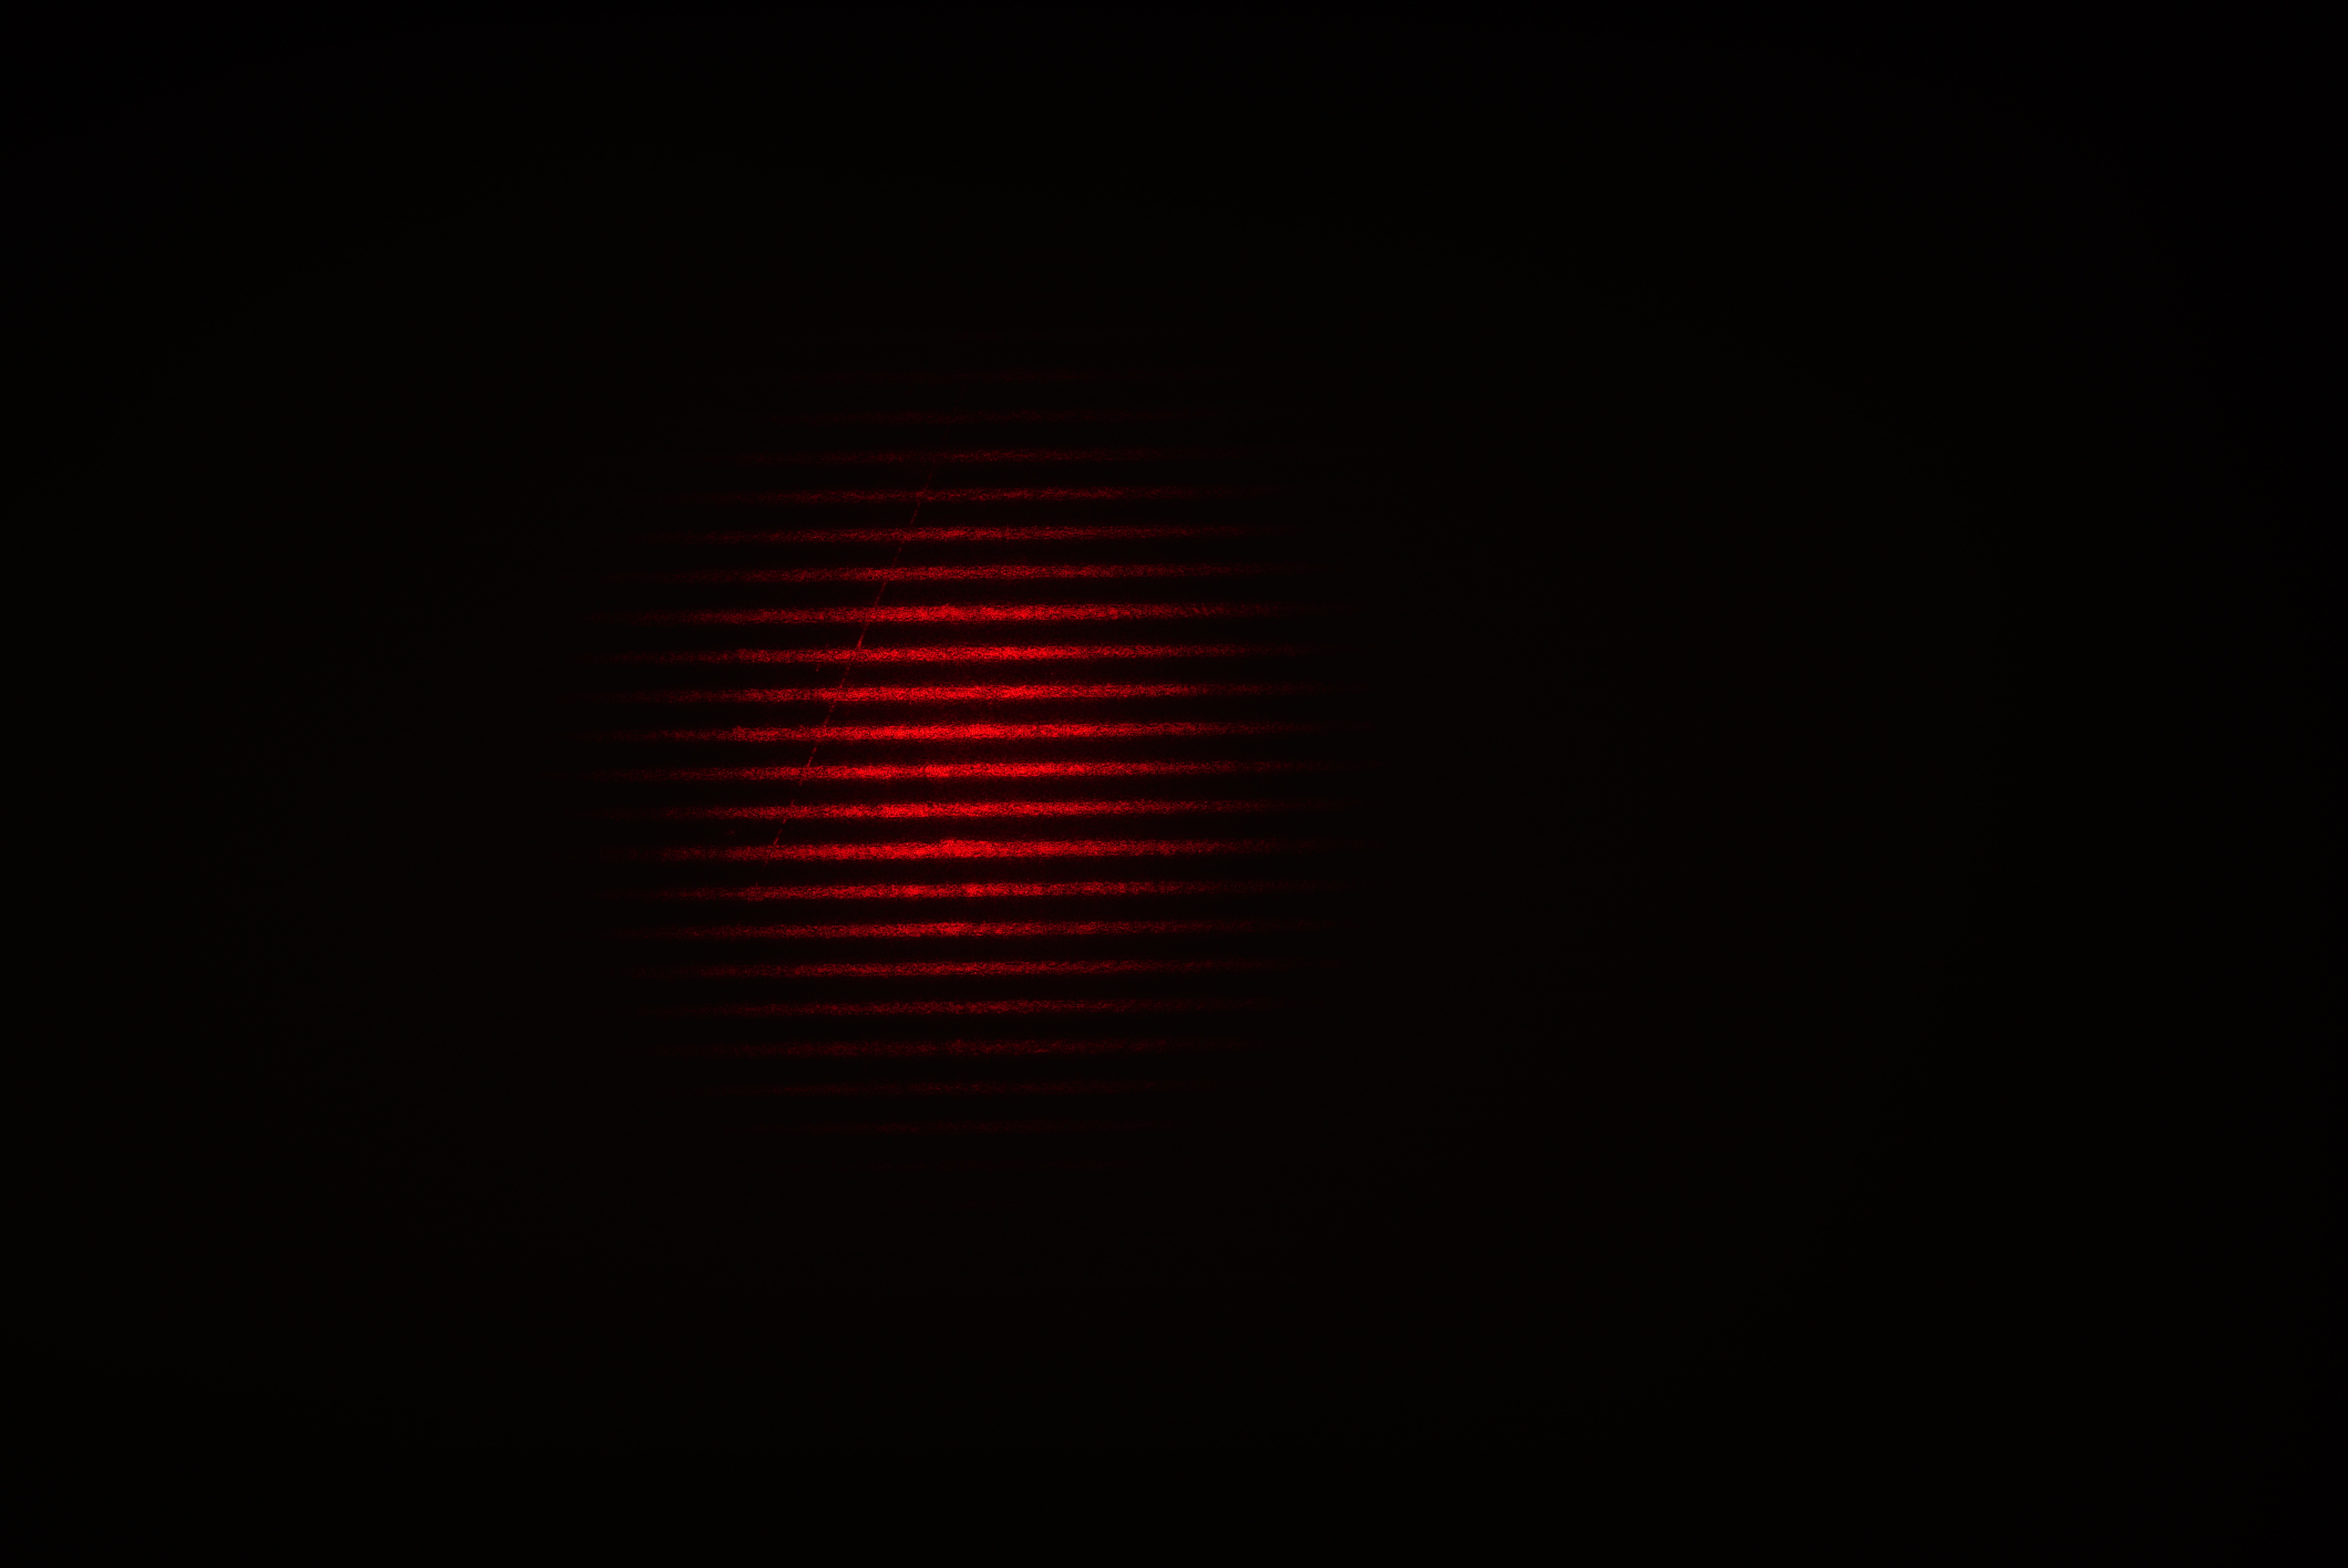
\includegraphics[ width = 0.95 \linewidth ]{figures/Inverse FT/DSC01516.JPG}
        \caption{The captured inverse FT using filter 4}
    \end{minipage}%
    \vspace{2cm}
    \begin{minipage}{0.45\textwidth}
        \centering
        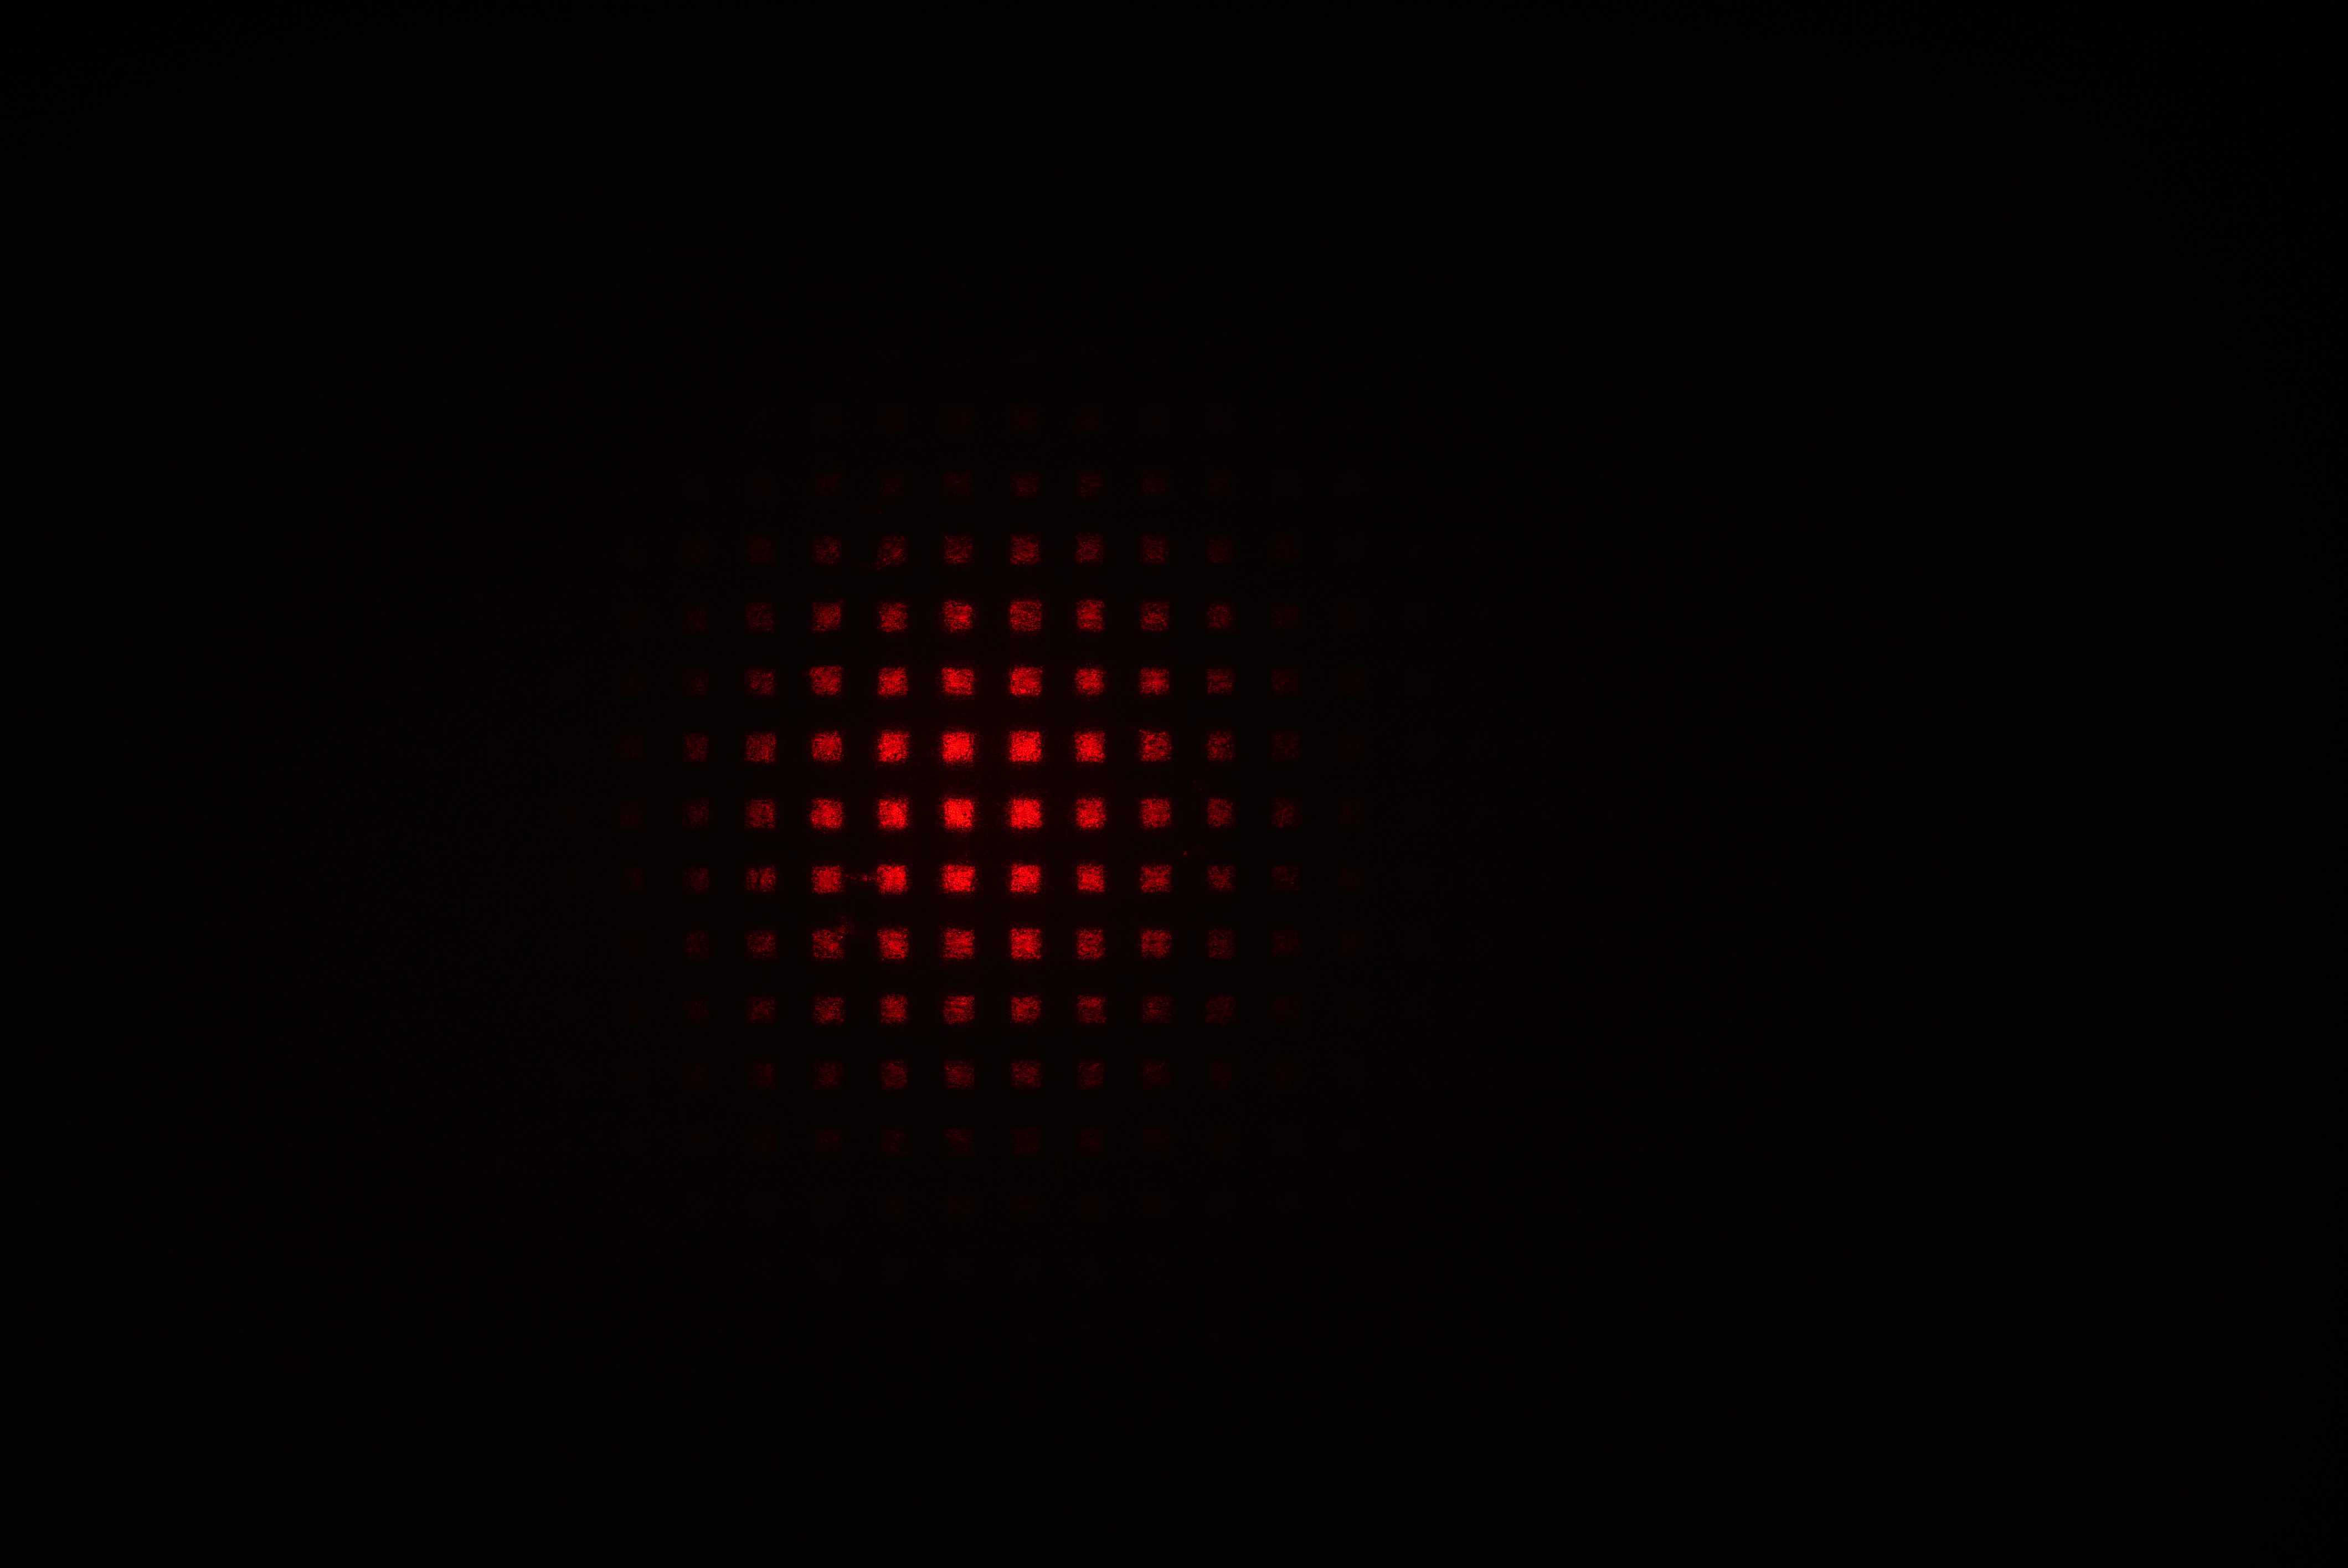
\includegraphics[ width = 0.95 \linewidth ]{figures/Inverse FT/DSC01519.JPG}
        \caption{The captured inverse FT using filter 5}
    \end{minipage}%
    \begin{minipage}{0.45\textwidth}
        \centering
        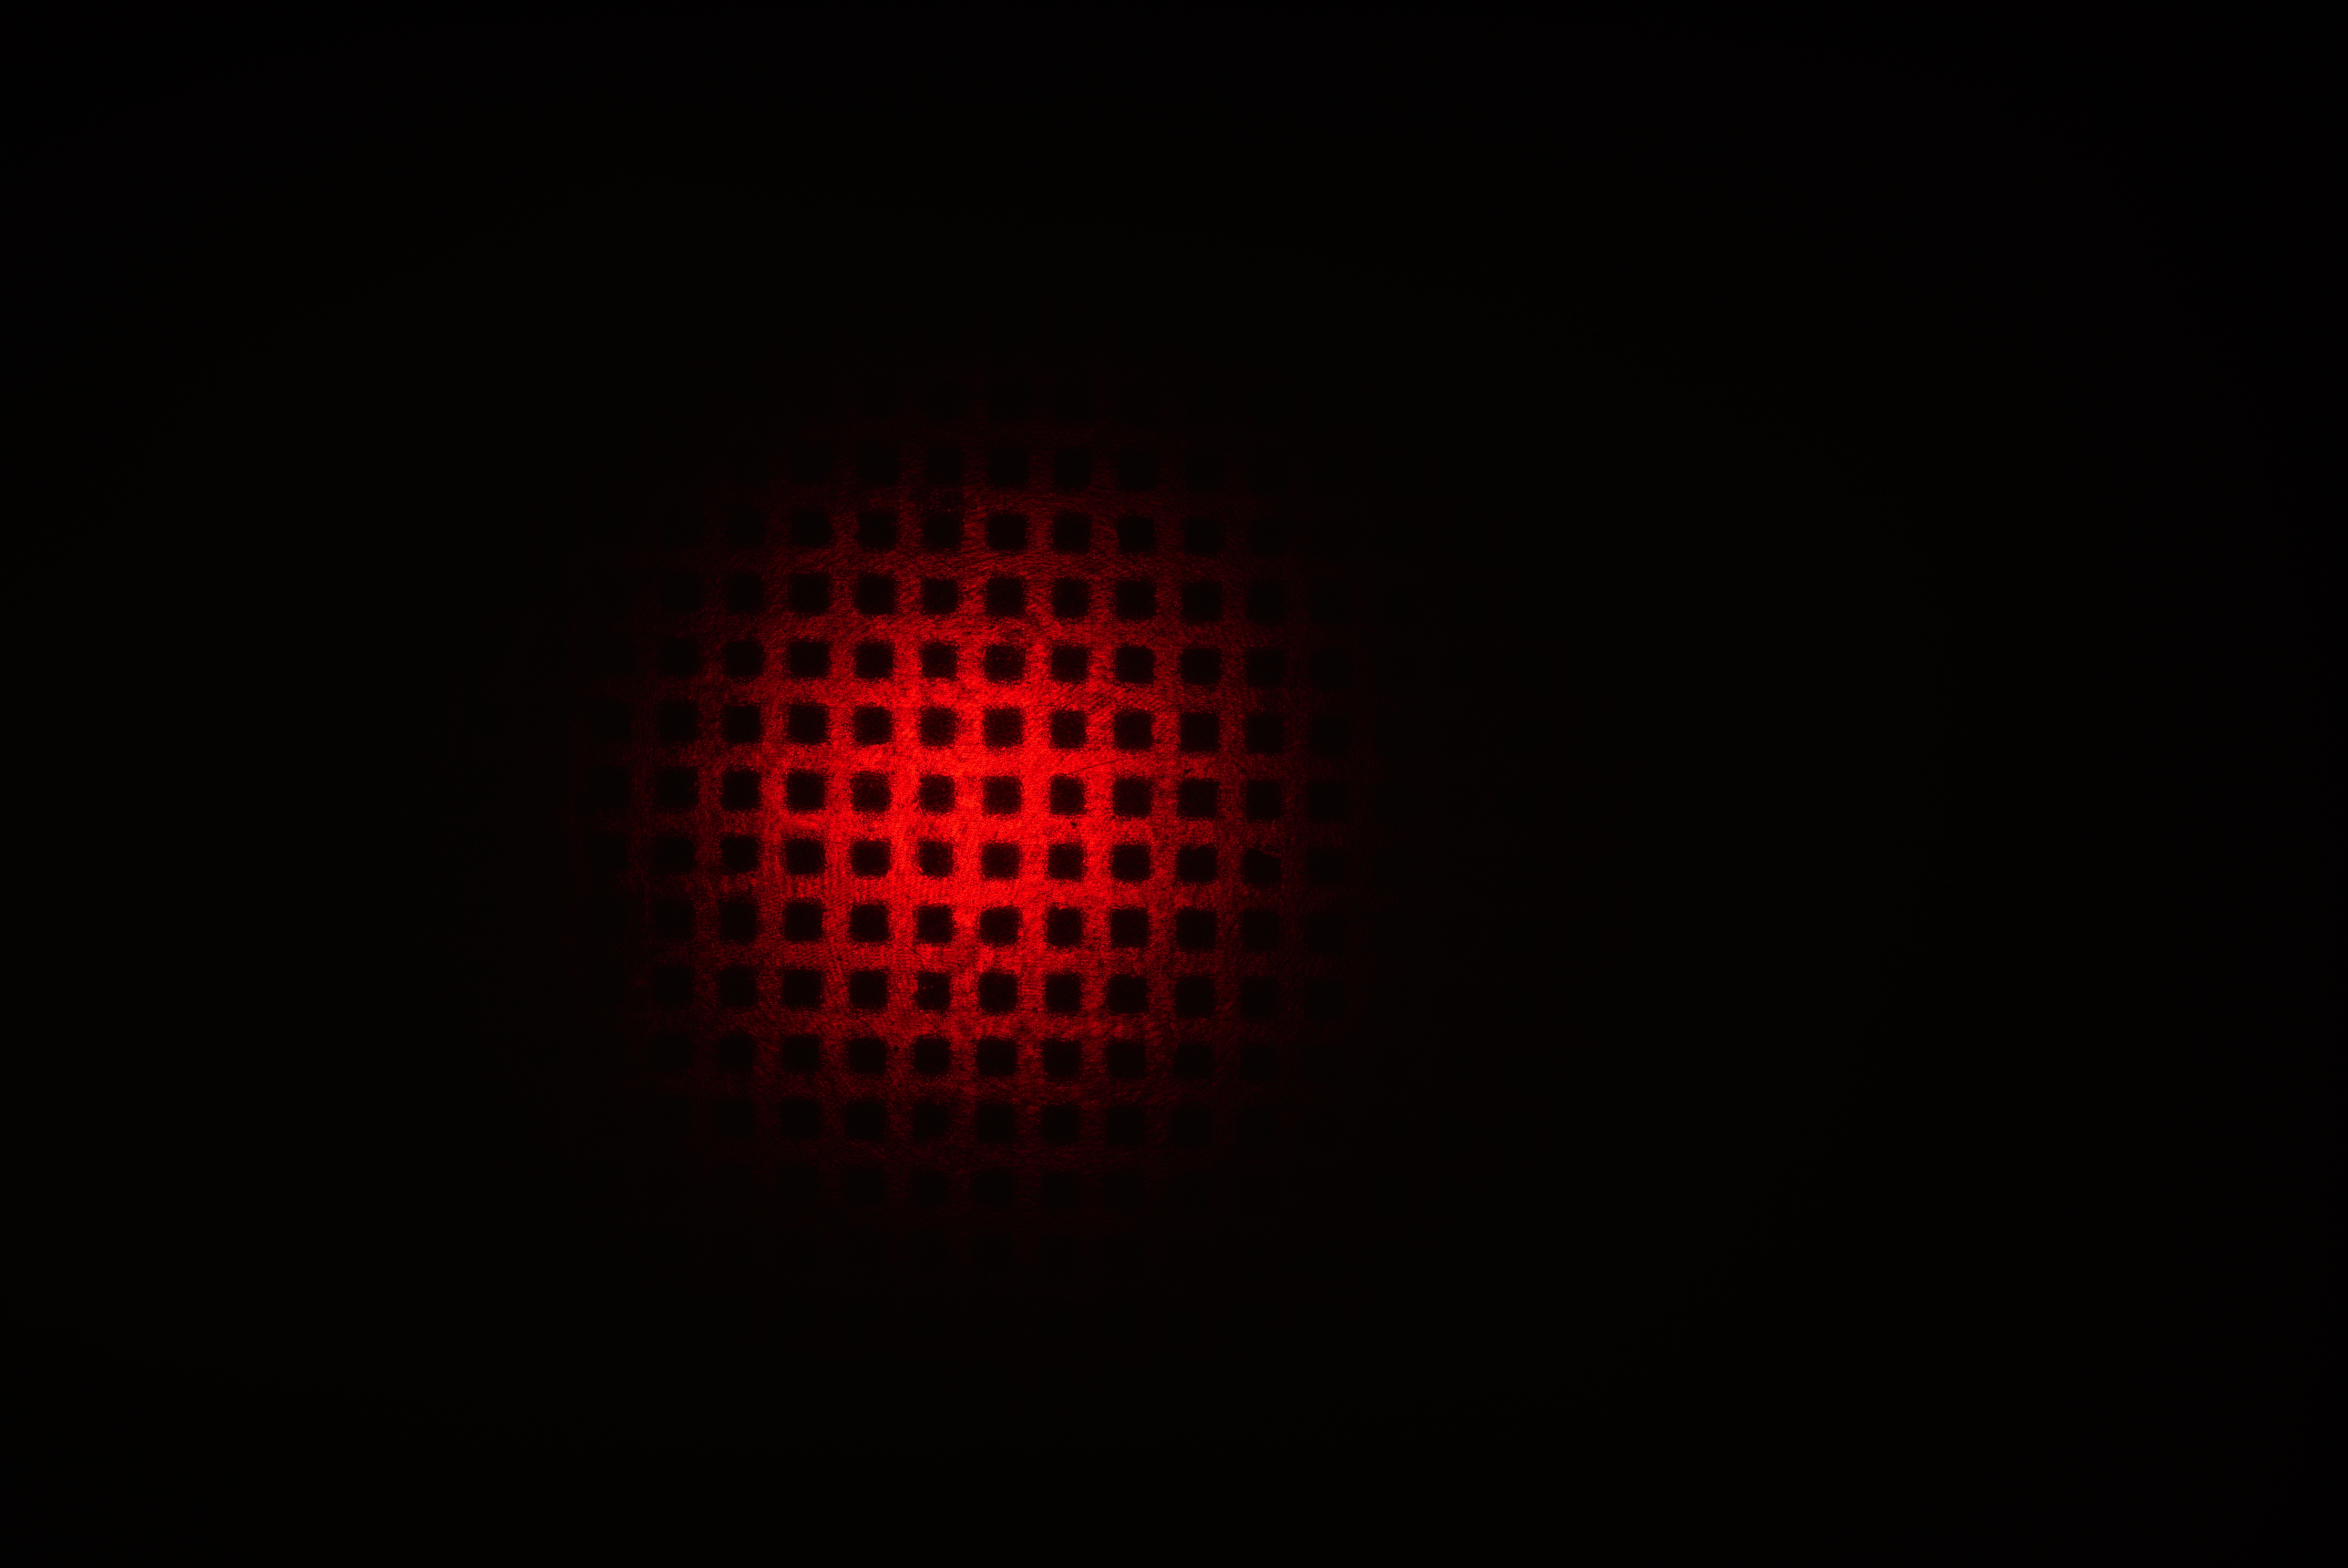
\includegraphics[ width = 0.95 \linewidth ]{figures/Inverse FT/DSC01522.JPG}
        \caption{The captured inverse FT using filter 6}
    \end{minipage}%
\end{figure}

\subsection{Calculated Fourier Transform}
\begin{figure}[H]
    \centering
    \begin{minipage}{0.45\textwidth}
        \centering
        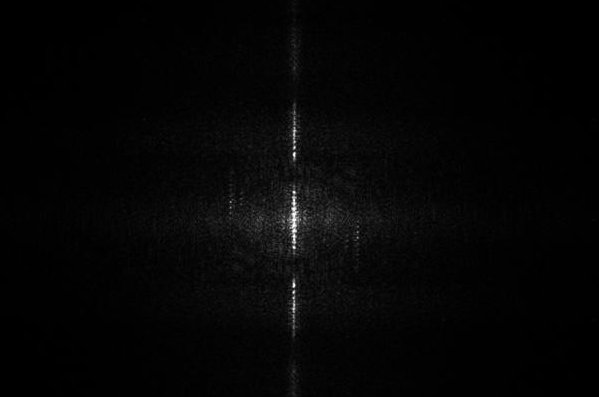
\includegraphics[ width = 0.95 \linewidth ]{figures/CalculatedFT/1505_FourierTransform_LinearPlot3.jpg}
        \caption{The calculated FT using filter 1}
    \end{minipage}%
    \begin{minipage}{0.45\textwidth}
        \centering
        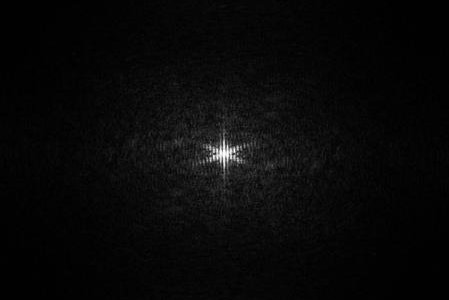
\includegraphics[ width = 0.95 \linewidth ]{figures/CalculatedFT/1508_FourierTransform_LinearPlot3.jpg}
        \caption{The calculated FT using filter 2}
    \end{minipage}%
    \vspace{2cm}
    \begin{minipage}{0.45\textwidth}
        \centering
        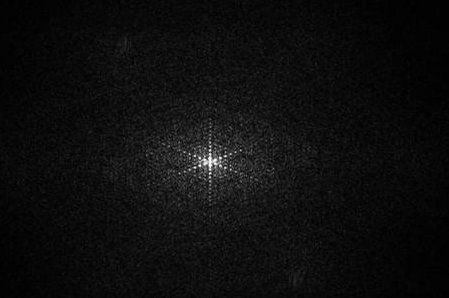
\includegraphics[ width = 0.95 \linewidth ]{figures/CalculatedFT/1511_FourierTransform_LinearPlot3.jpg}
        \caption{The calculated FT using filter 3}
    \end{minipage}%
    \begin{minipage}{0.45\textwidth}
        \centering
        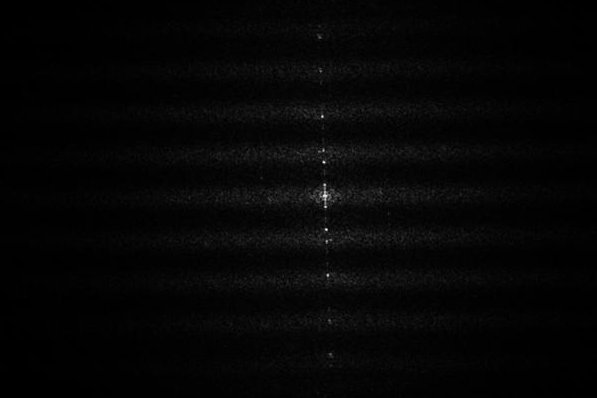
\includegraphics[ width = 0.95 \linewidth ]{figures/CalculatedFT/1514_FourierTransform_LinearPlot3.jpg}
        \caption{The calculated FT using filter 4}
    \end{minipage}%
    \vspace{2cm}
    \begin{minipage}{0.45\textwidth}
        \centering
        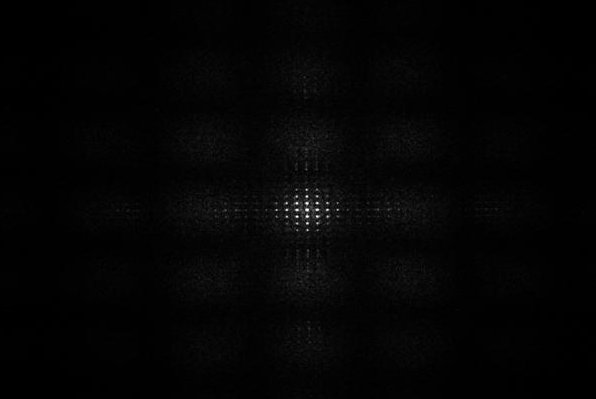
\includegraphics[ width = 0.95 \linewidth ]{figures/CalculatedFT/1517_FourierTransform_LinearPlot3.jpg}
        \caption{The calculated FT using filter 5}
    \end{minipage}%
    \begin{minipage}{0.45\textwidth}
        \centering
        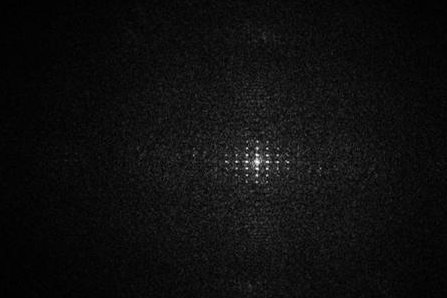
\includegraphics[ width = 0.95 \linewidth ]{figures/CalculatedFT/1520_FourierTransform_LinearPlot3.jpg}
        \caption{The calculated FT using filter 6}
    \end{minipage}%
\end{figure}

\subsection{Captured Inverse Fourier Transform with the Aperture Involved}
All of the captured images below were with filter 3.
\begin{figure}[H]
    \centering
    \begin{minipage}[t]{0.45\textwidth}
        \centering
        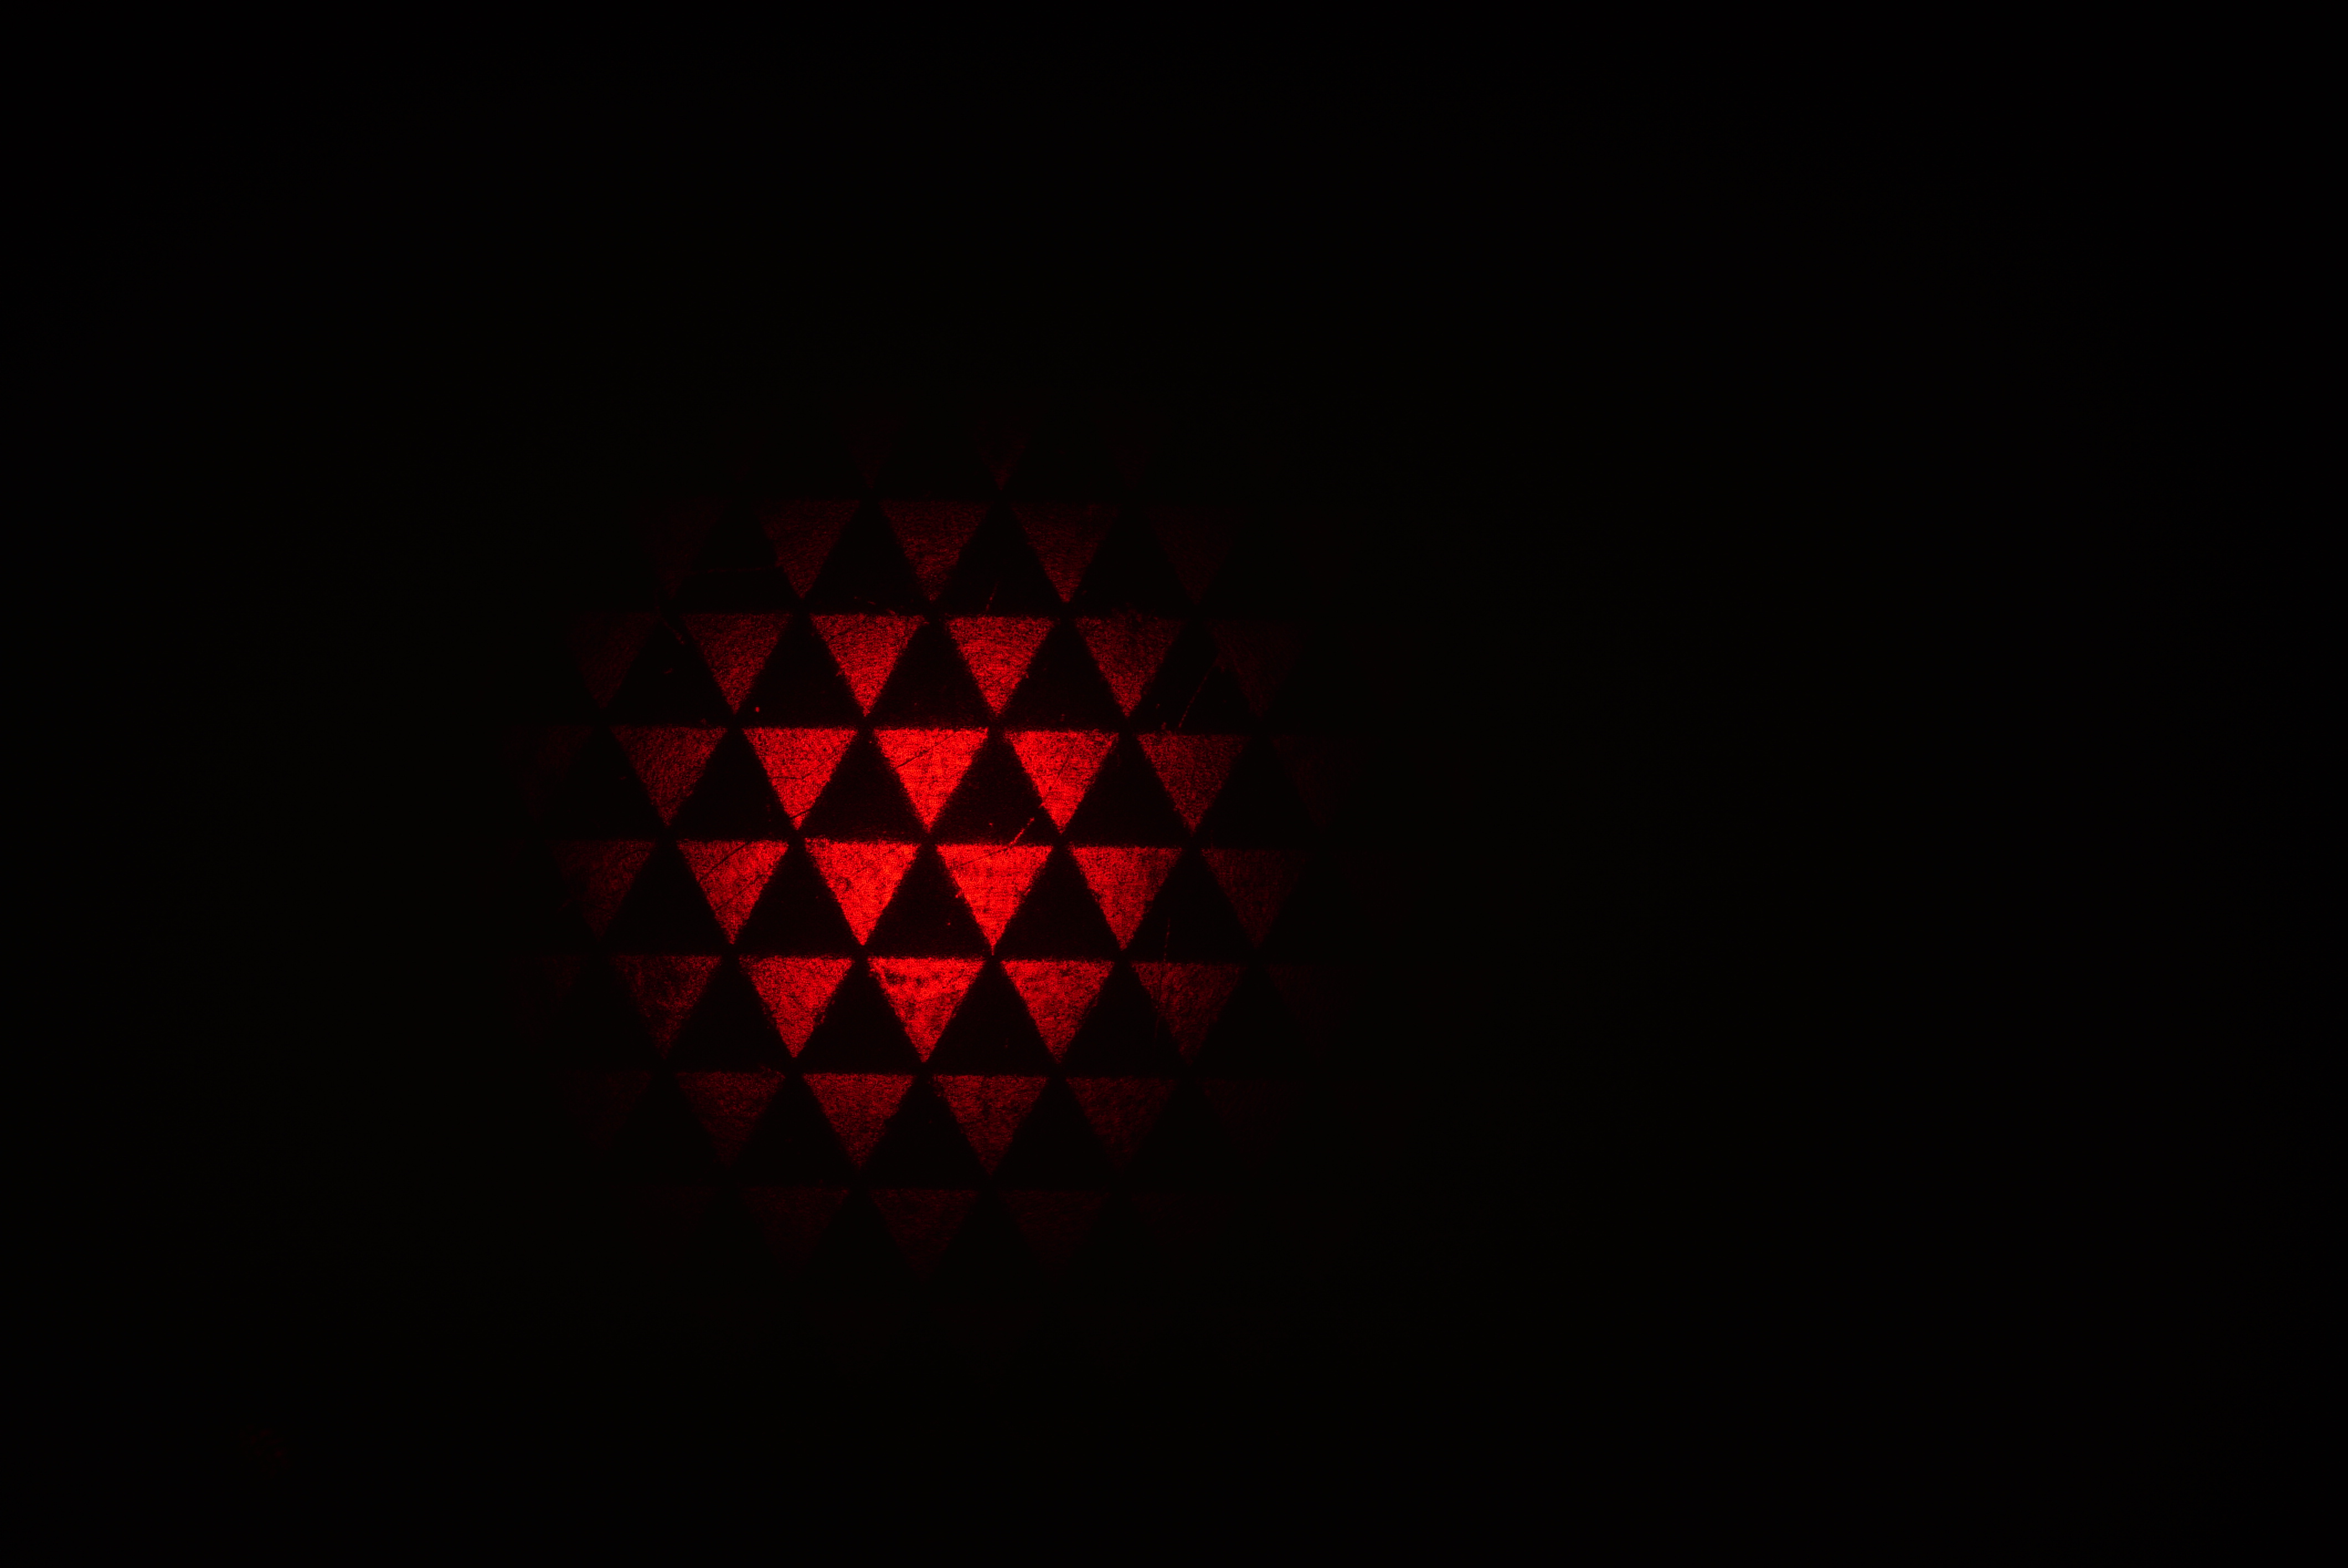
\includegraphics[ width = 0.95 \linewidth ]{figures/AperatureImages/DSC01549.JPG}
        \caption{The captured inverse Fourier transform using no aperture}
    \end{minipage}%
    \hspace{0.5cm}
    \begin{minipage}[t]{0.45\textwidth}
        \centering
        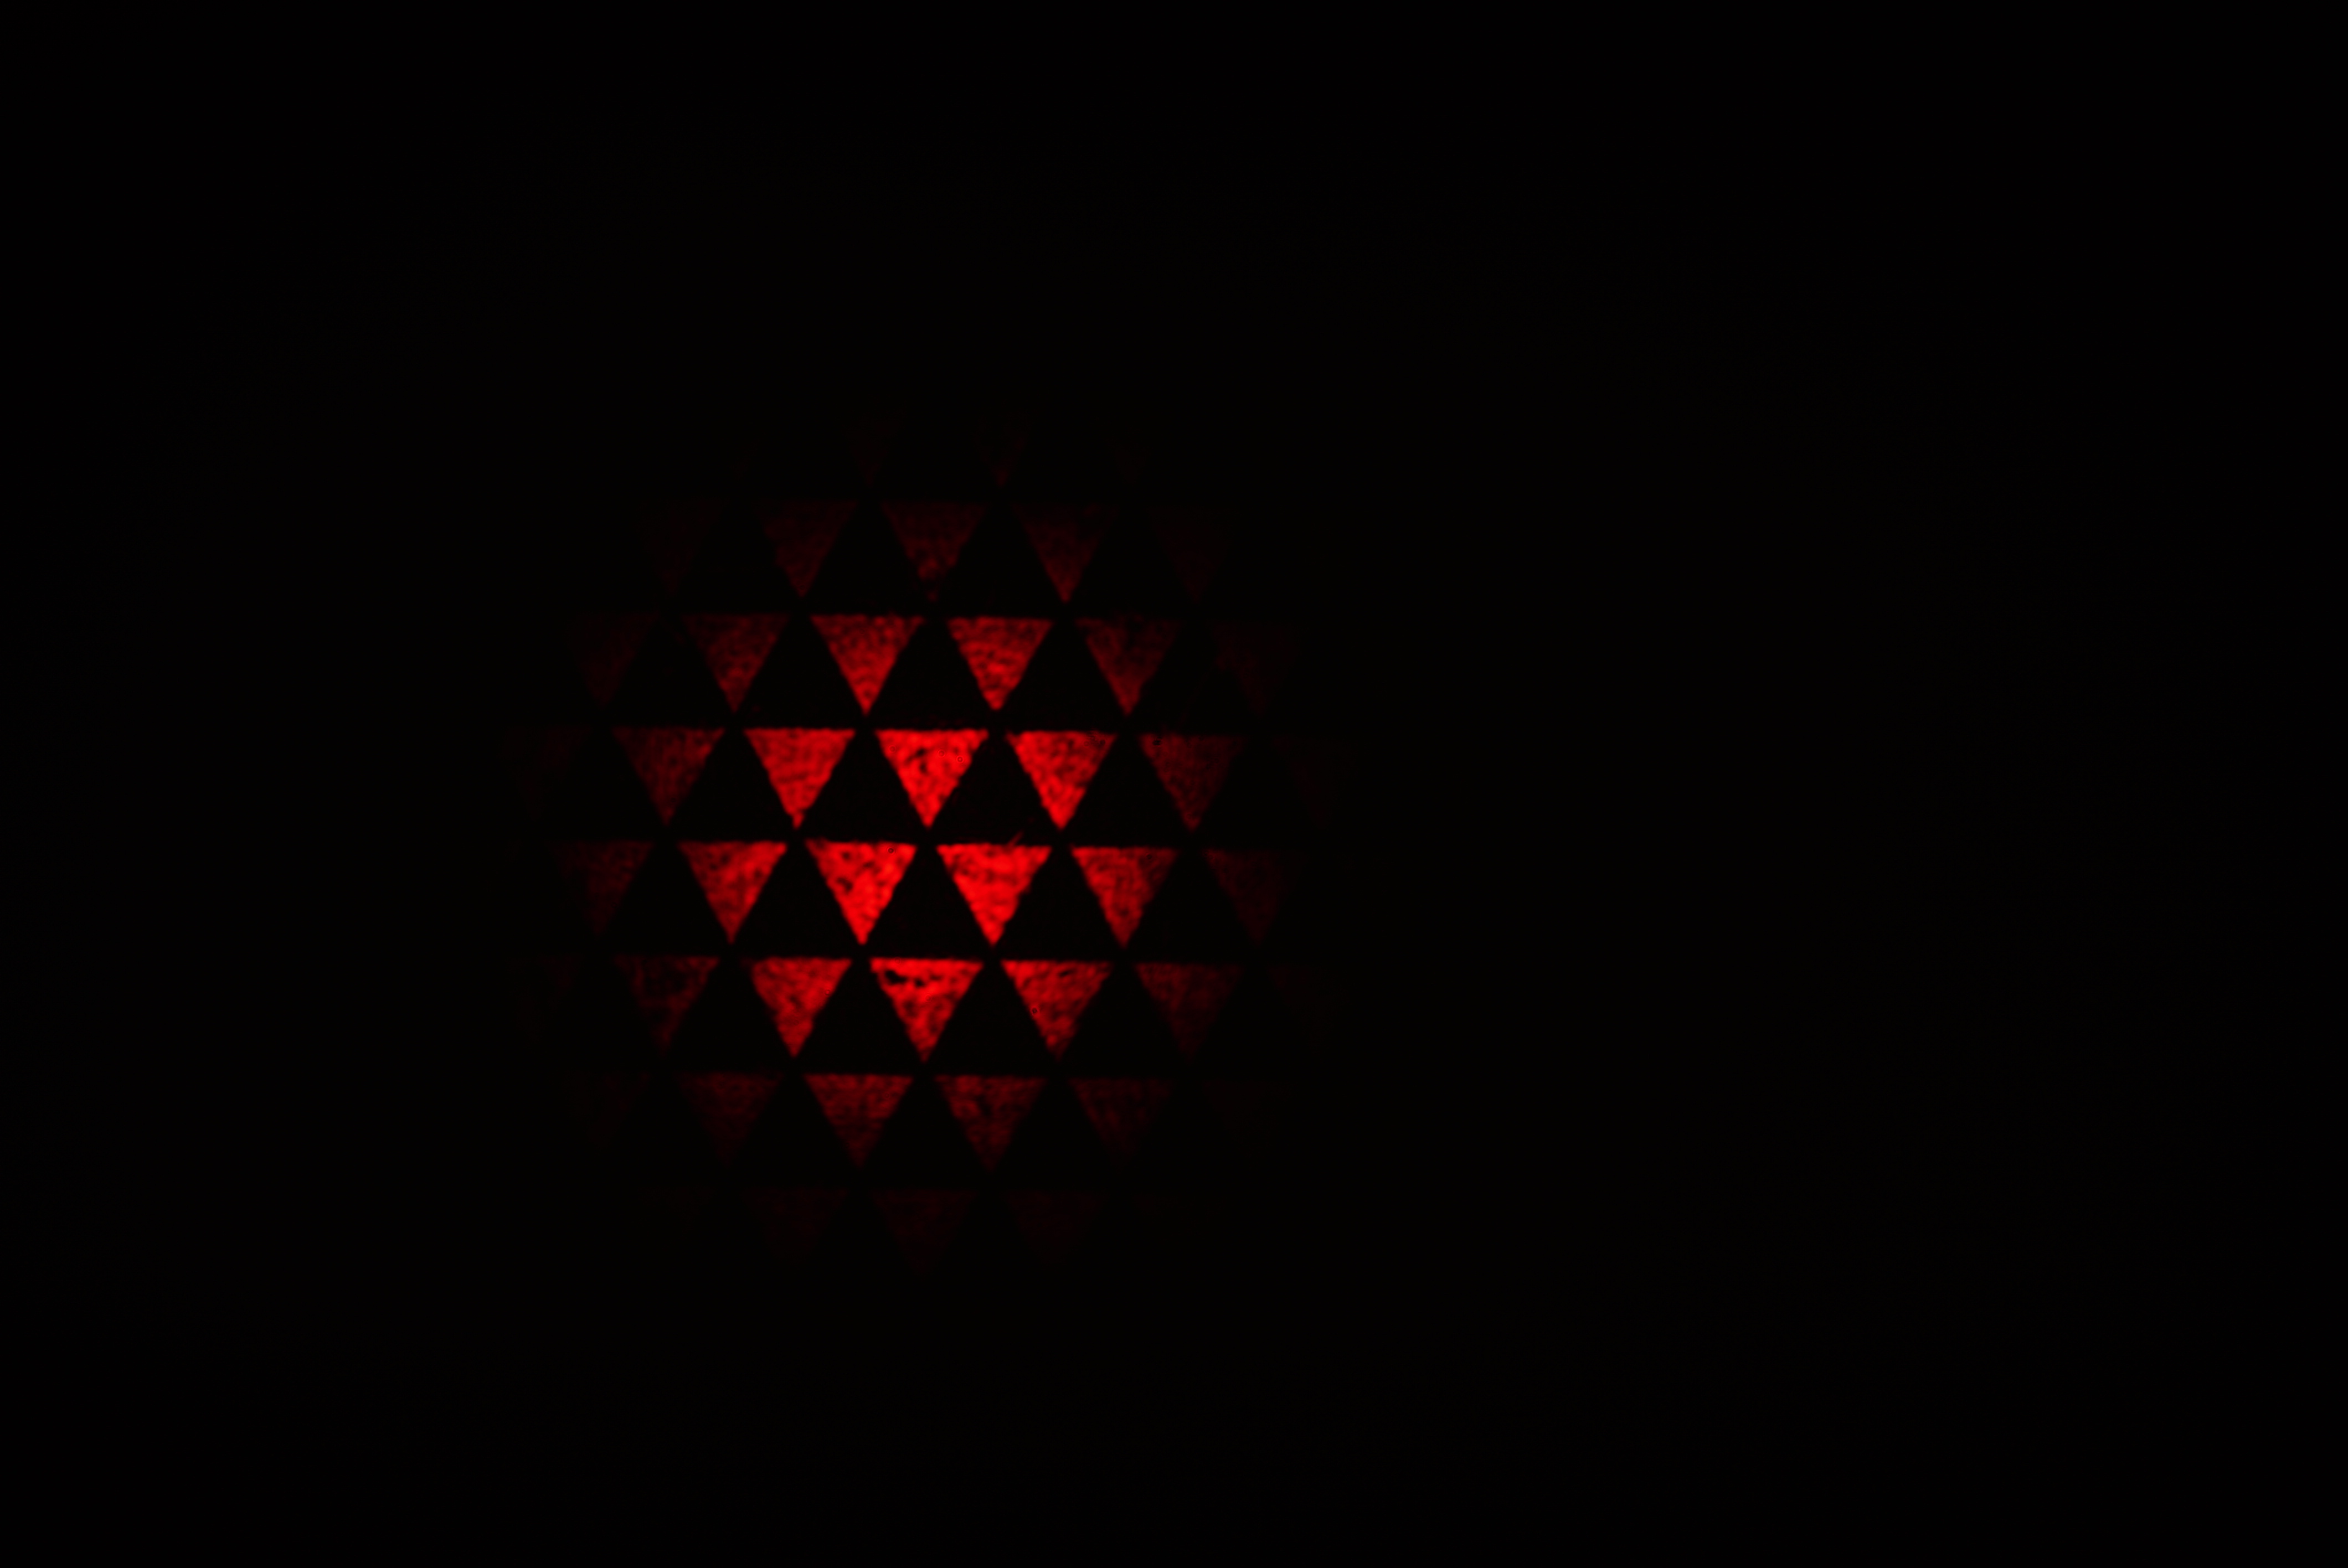
\includegraphics[ width = 0.95 \linewidth ]{figures/AperatureImages/DSC01548.JPG}
        \caption{The captured inverse Fourier transform using the aperture with a diameter of $2.0 \ \si{mm}$}
    \end{minipage}%
    \vspace{1.5cm}
    \begin{minipage}[t]{0.45\textwidth}
        \centering
        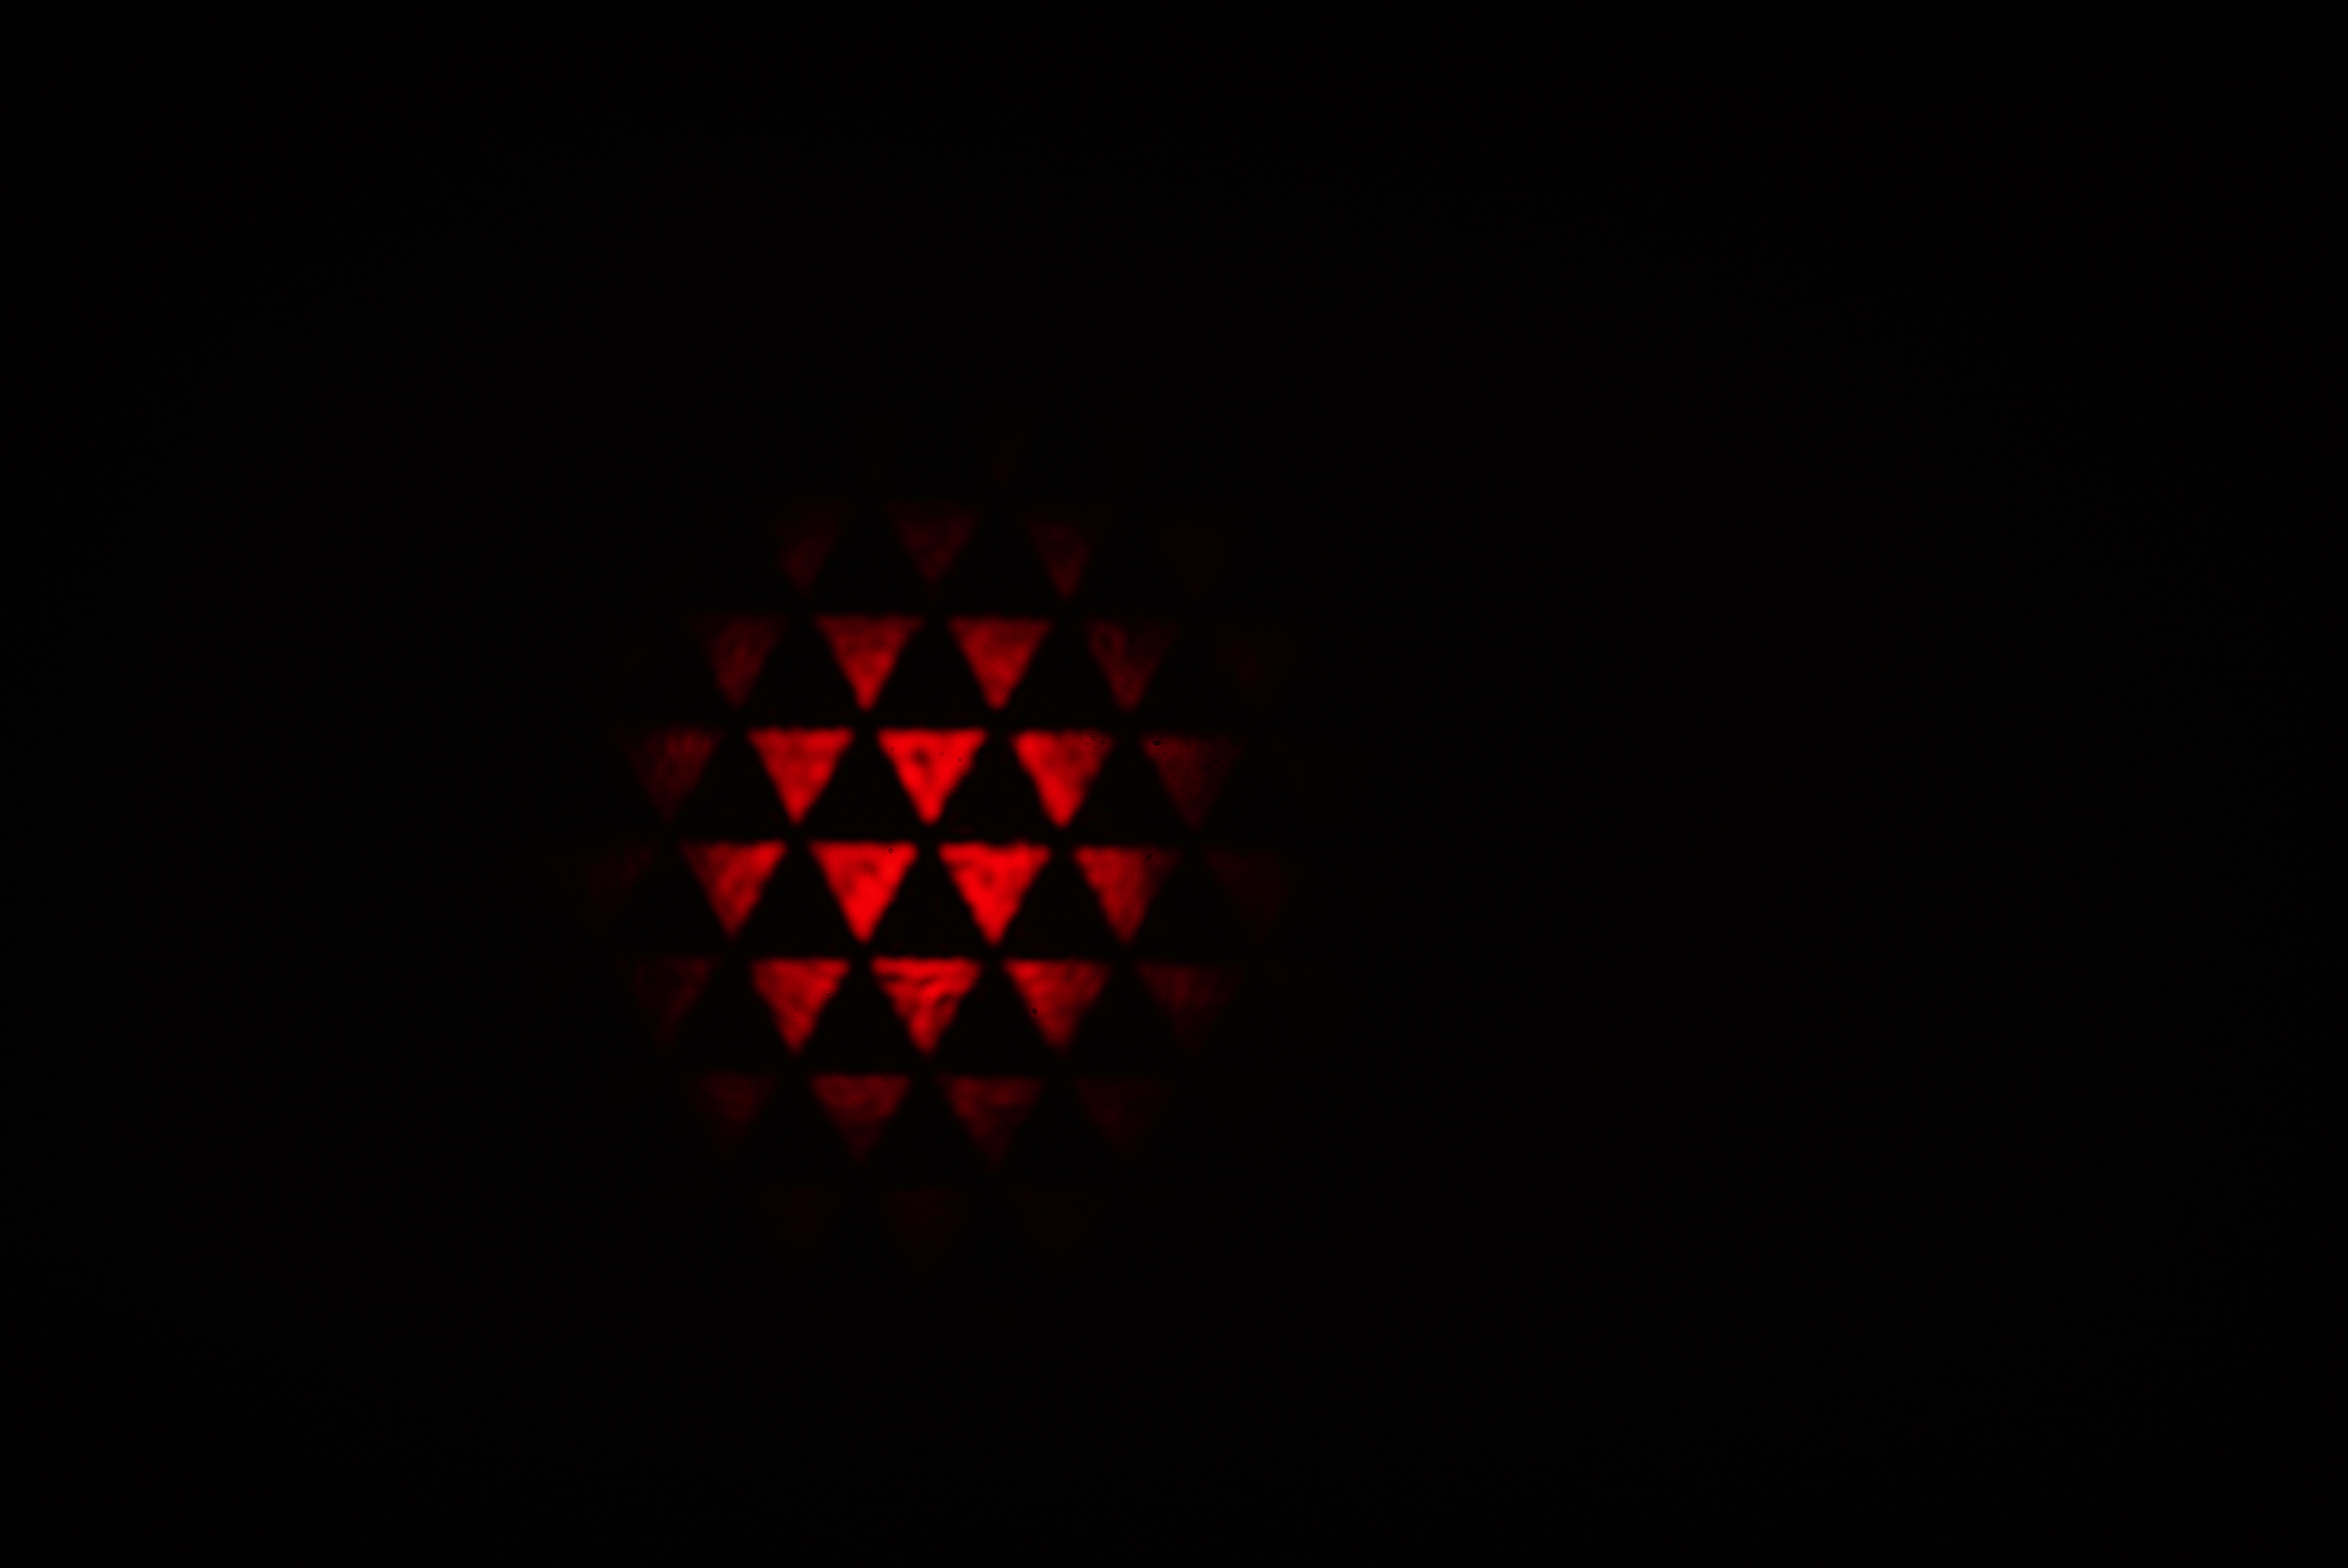
\includegraphics[ width = 0.95 \linewidth ]{figures/AperatureImages/DSC01547.JPG}
        \caption{The captured inverse Fourier transform using the aperture with a diameter of $1.0 \ \si{mm}$}
    \end{minipage}%
    \hspace{0.5cm}
    \begin{minipage}[t]{0.45\textwidth}
        \centering
        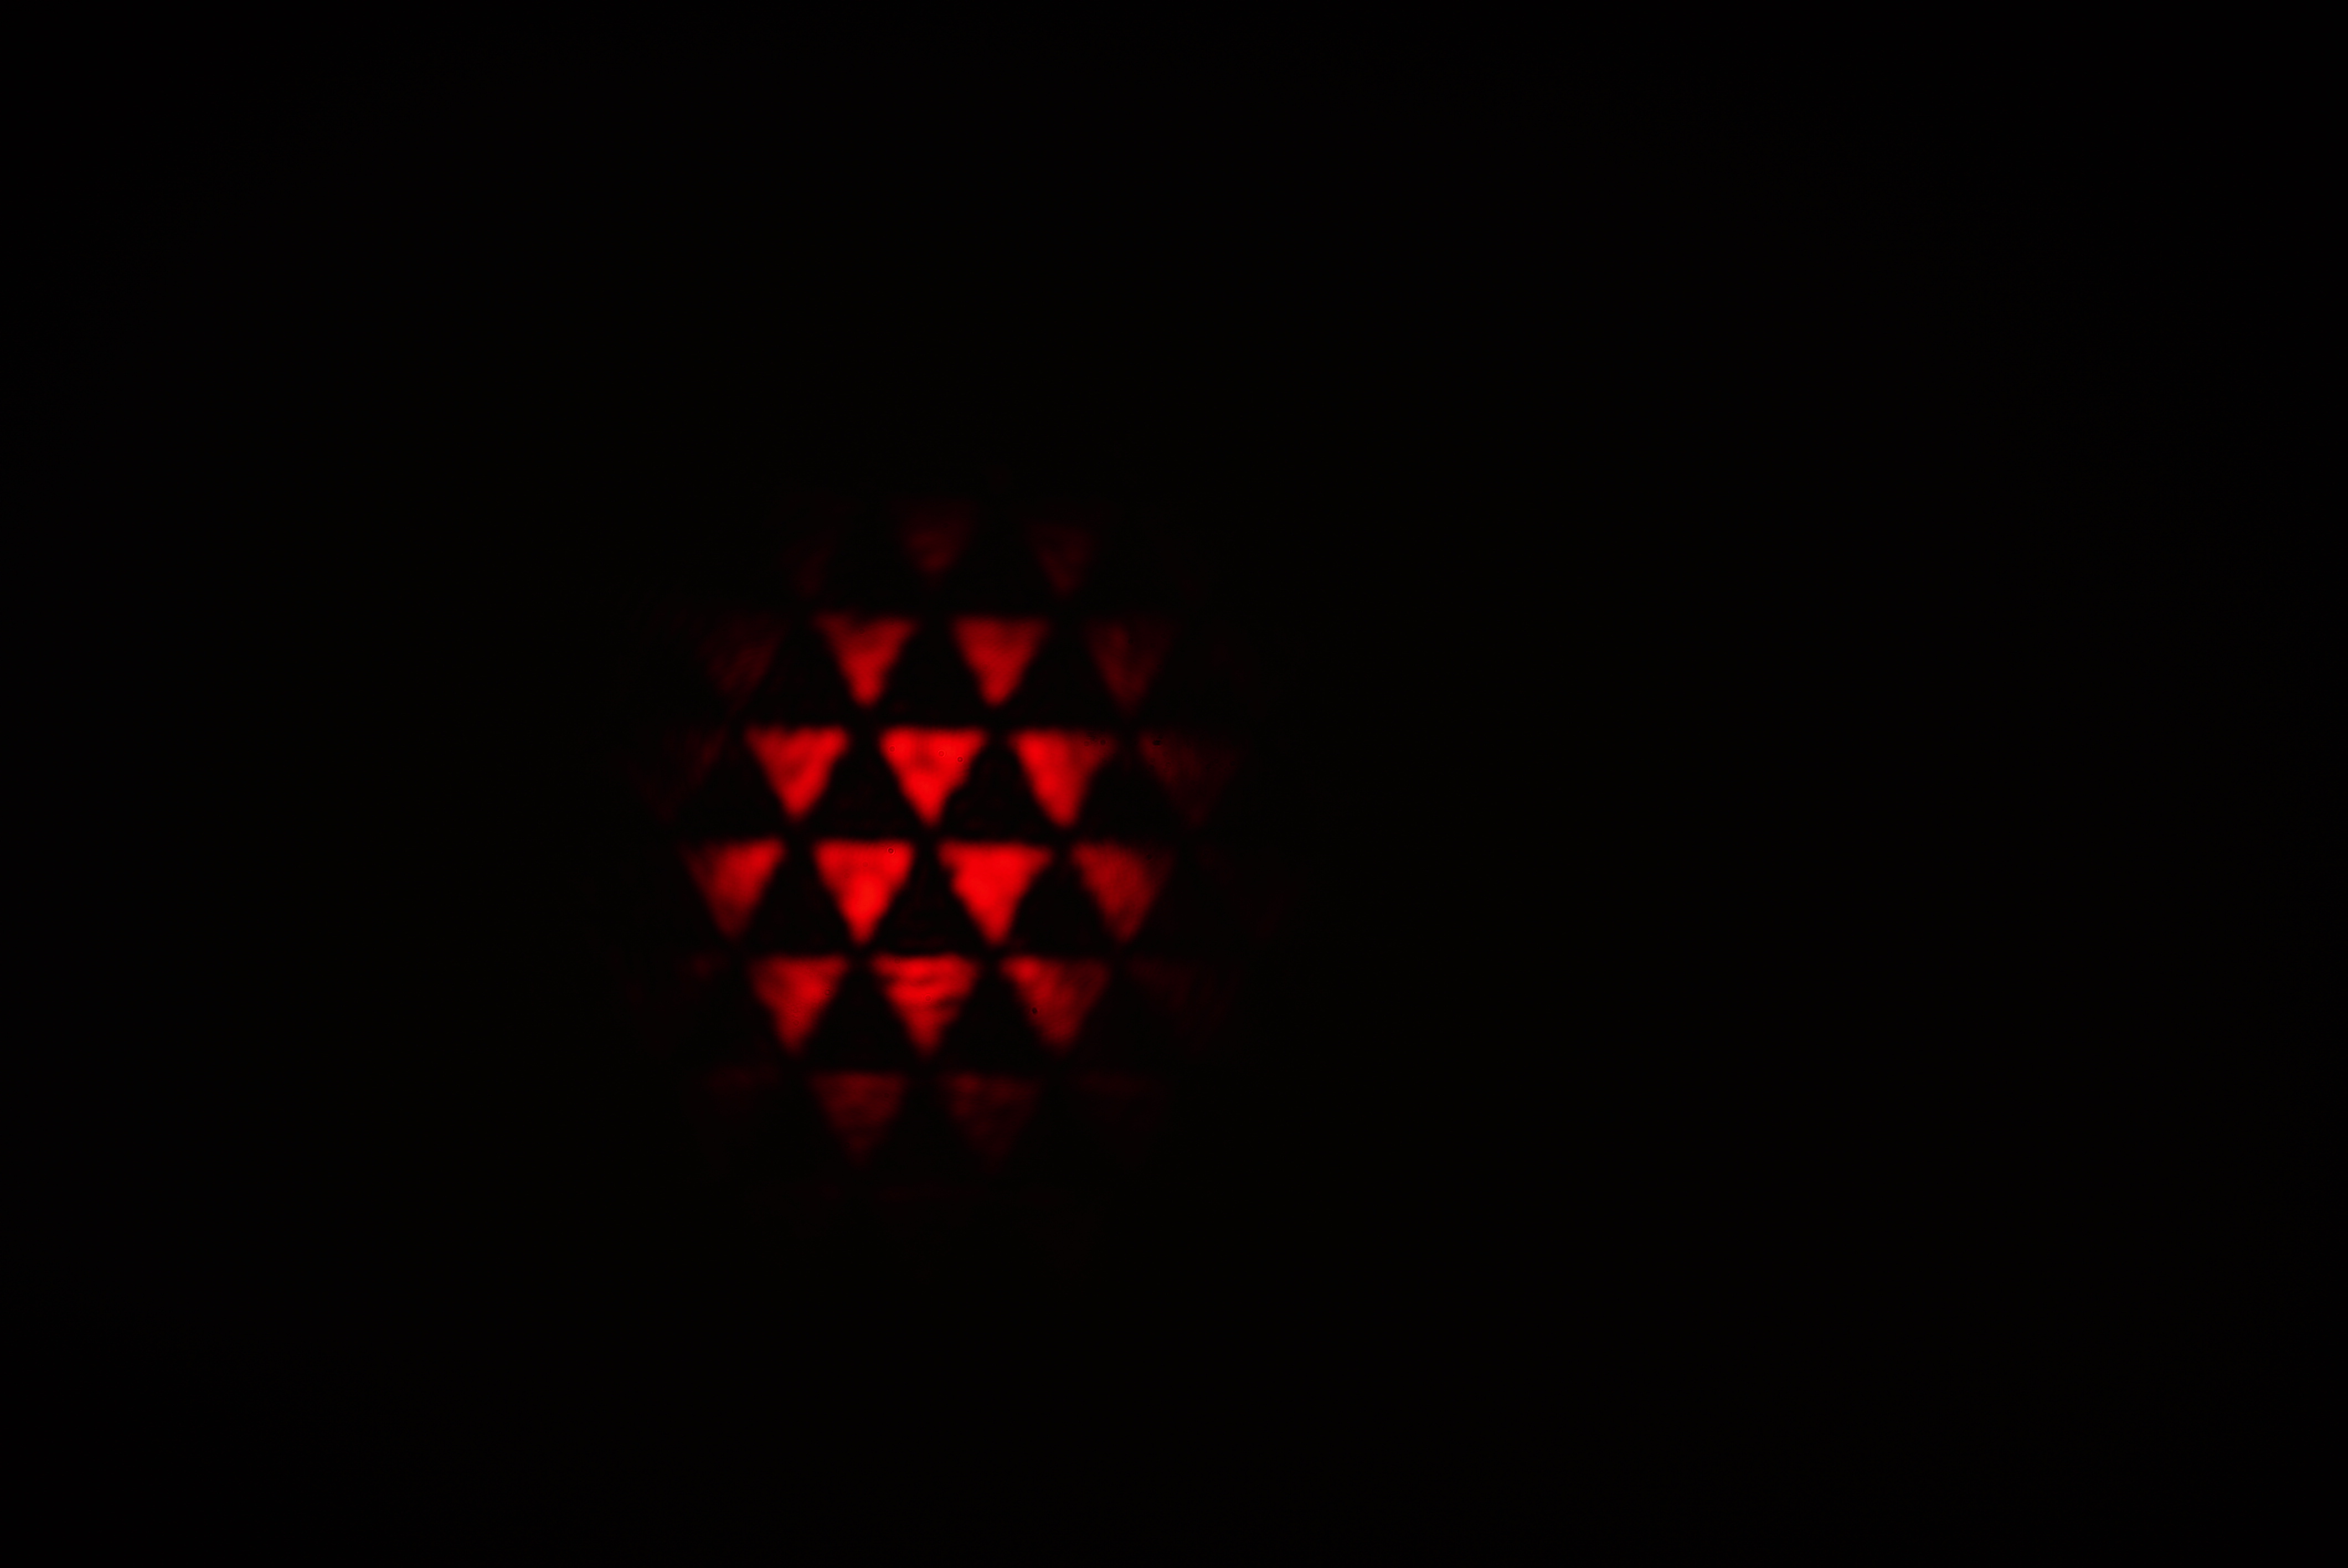
\includegraphics[ width = 0.95 \linewidth ]{figures/AperatureImages/DSC01546.JPG}
        \caption{The captured inverse Fourier transform using the aperture with a diameter of $0.70 \ \si{mm}$}
    \end{minipage}%
    \vspace{1.5cm}
    \begin{minipage}[t]{0.45\textwidth}
        \centering
        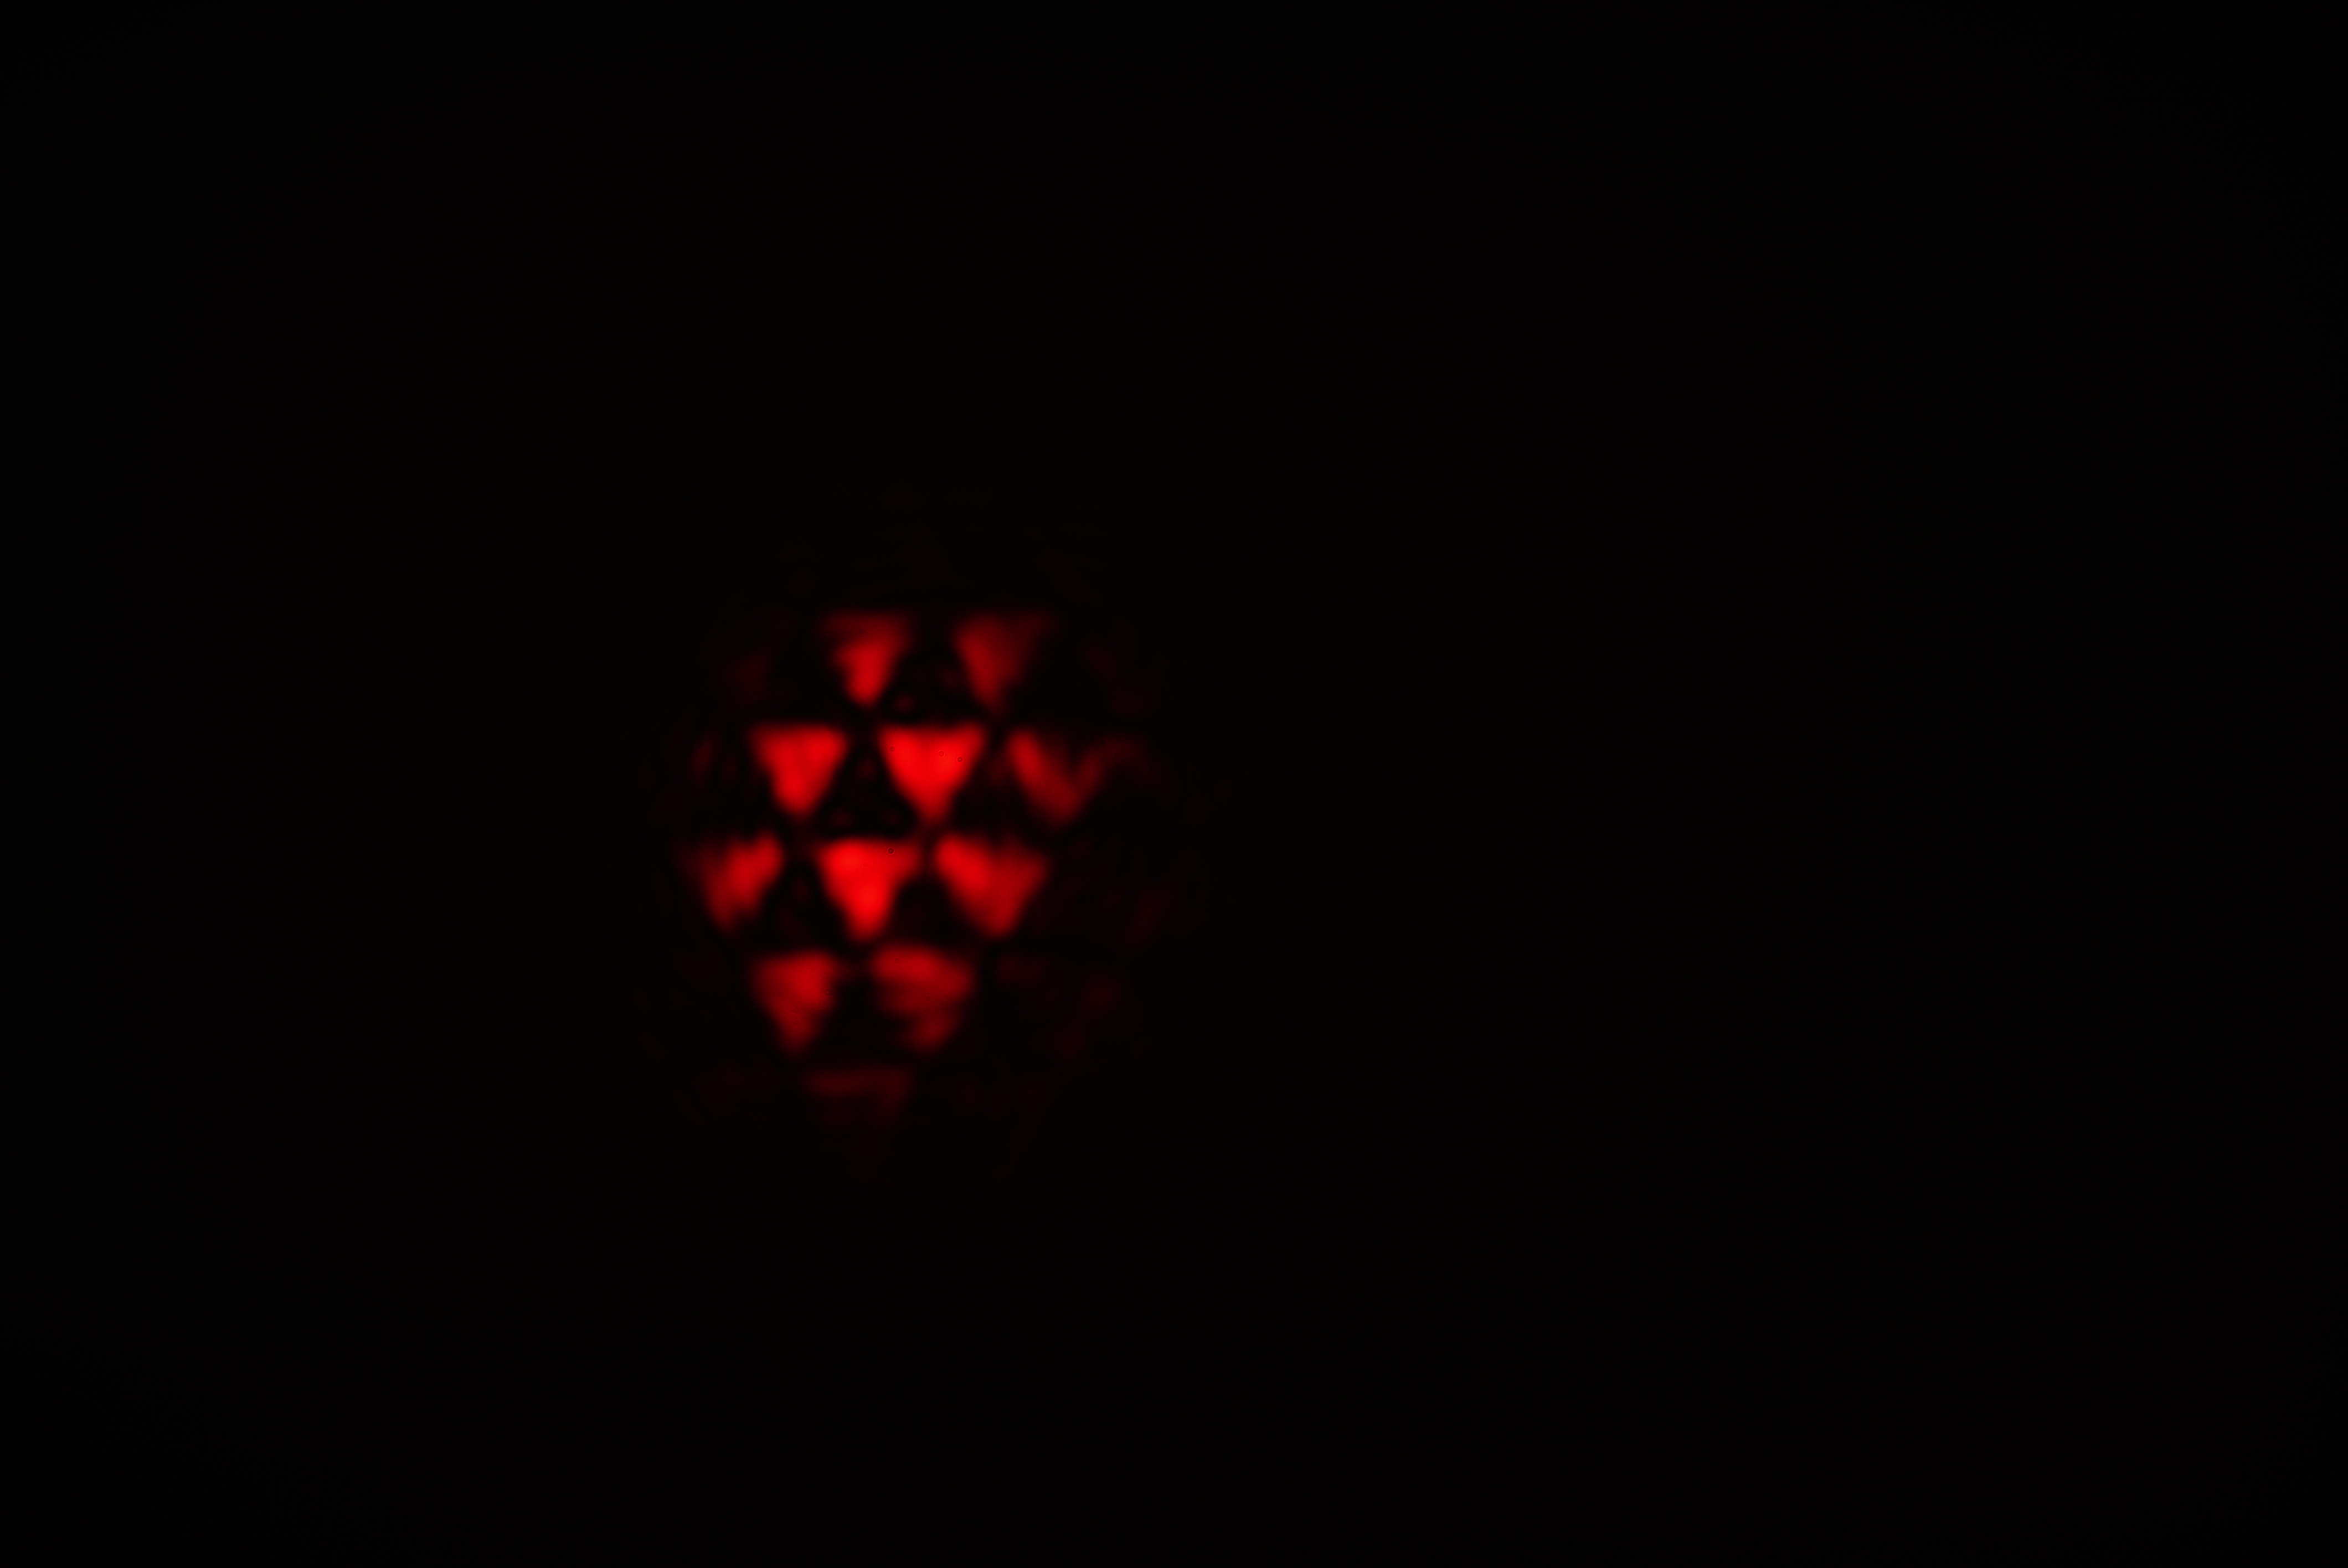
\includegraphics[ width = 0.95 \linewidth ]{figures/AperatureImages/DSC01545.JPG}
        \caption{The captured inverse Fourier transform using the aperture with a diameter of $0.50 \ \si{mm}$}
    \end{minipage}%
    \hspace{0.5cm}
    \begin{minipage}[t]{0.45\textwidth}
        \centering
        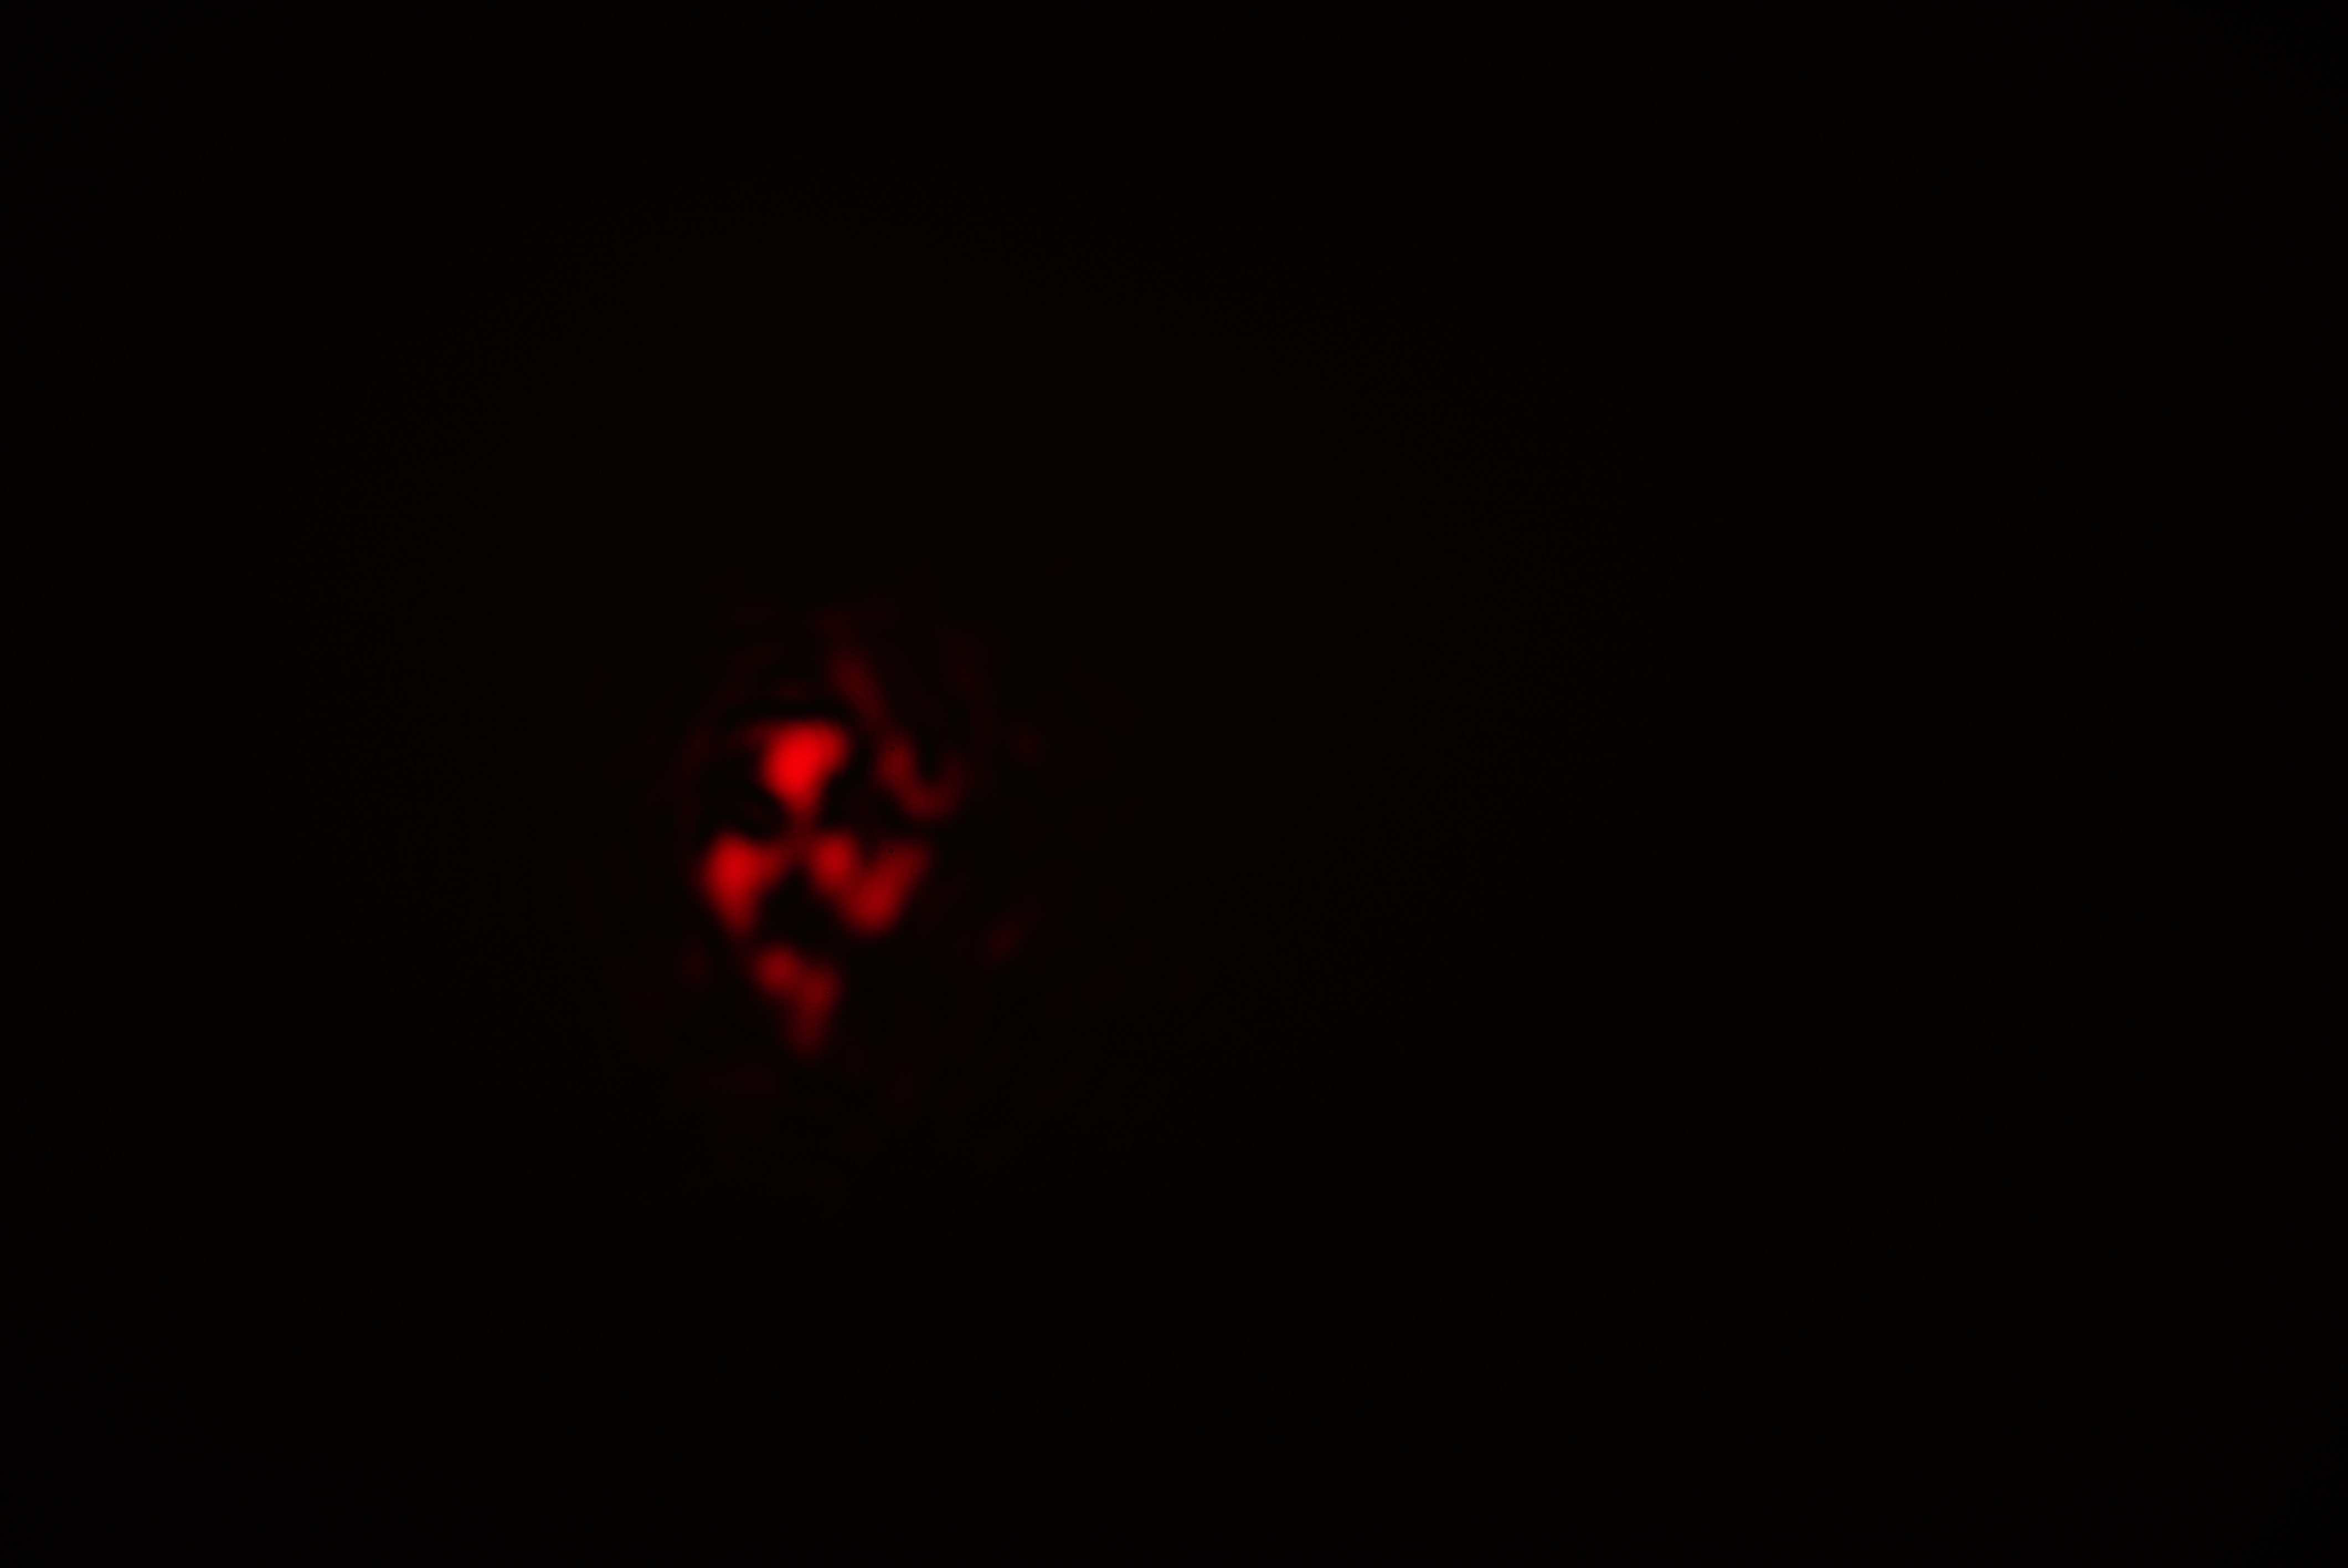
\includegraphics[ width = 0.95 \linewidth ]{figures/AperatureImages/DSC01544.JPG}
        \caption{The captured inverse Fourier transform using the aperture with a diameter of $0.30 \ \si{mm}$}
    \end{minipage}%
\end{figure}

\subsection{Calculated Fourier Transform with the Aperture Involved}
We calculated all of Fourier transforms of the image produced by using filter 3.
\begin{figure}[H]
    \centering
    \begin{minipage}[t]{0.45\textwidth}
        \centering
        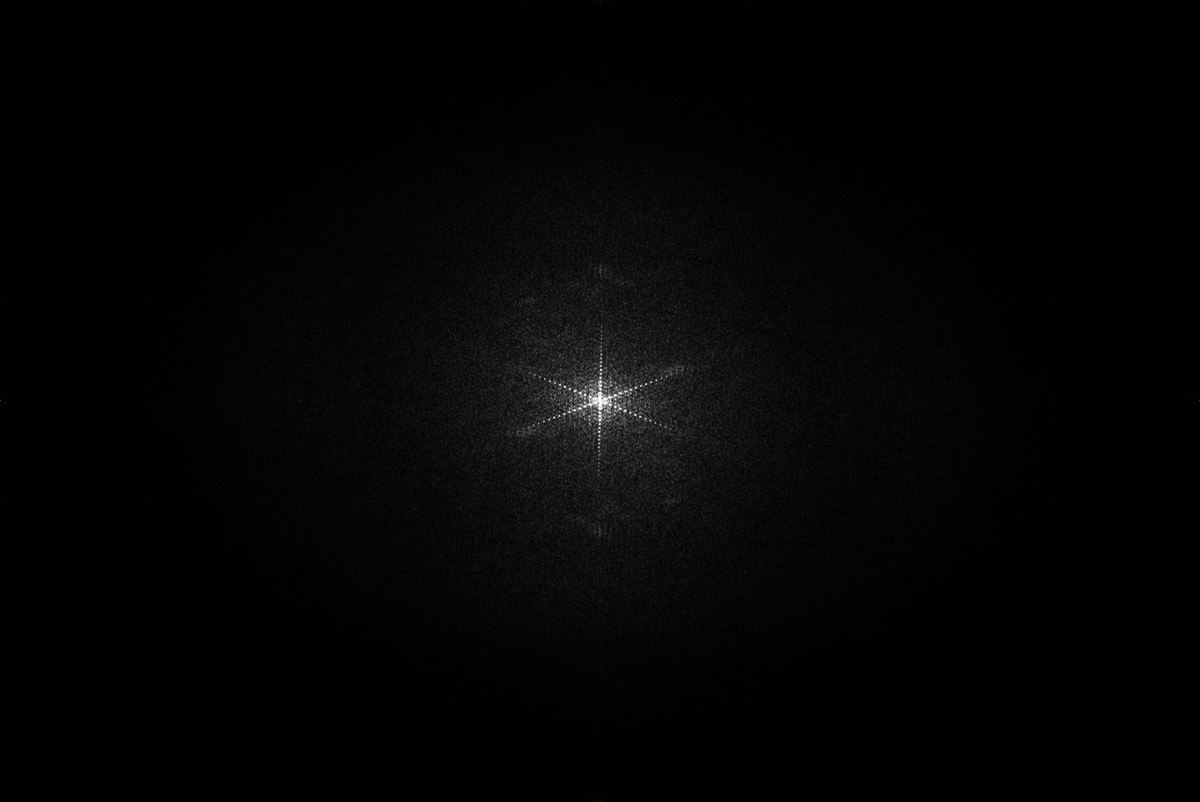
\includegraphics[ width = 0.95 \linewidth ]{figures/CalculatedFT/1549_FT_LinearPlot.png}
        \caption{The calculated FT with no aperture involved}
    \end{minipage}%
    \hspace{0.5cm}
    \begin{minipage}[t]{0.45\textwidth}
        \centering
        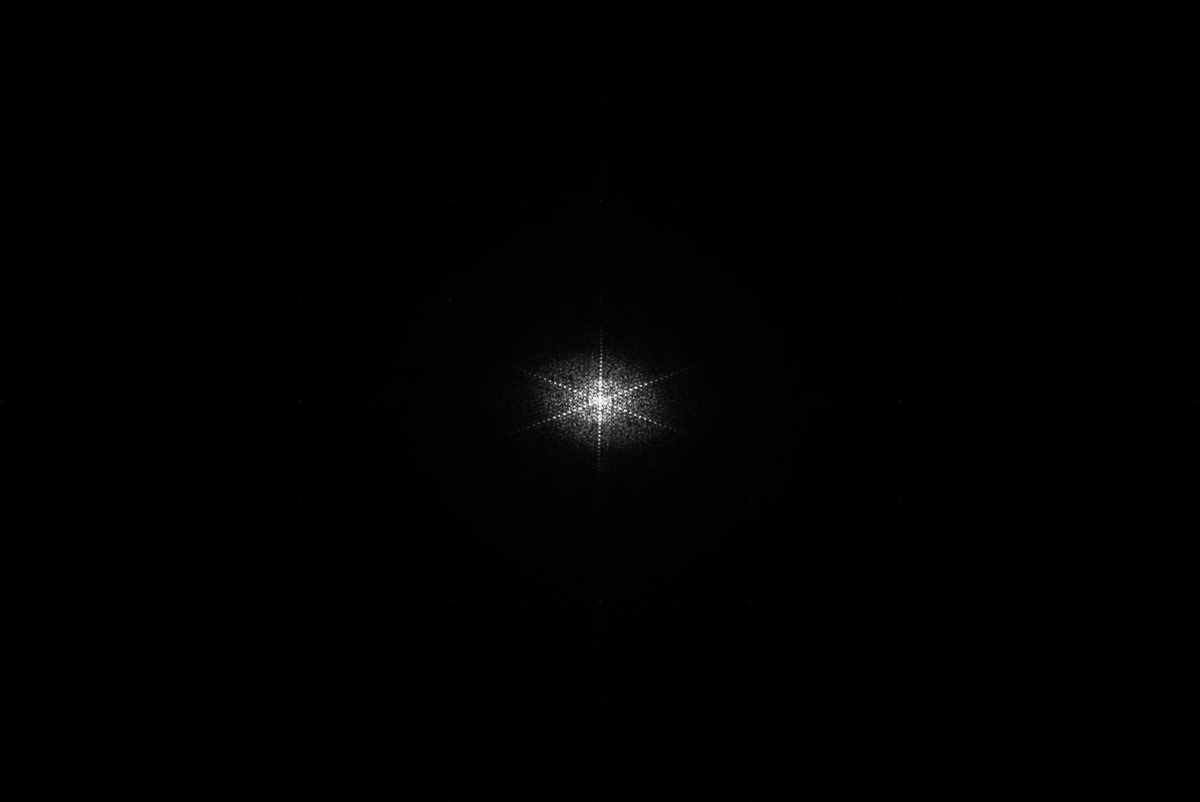
\includegraphics[ width = 0.95 \linewidth ]{figures/CalculatedFT/1548_FT_LinearPlot.png}
        \caption{The calculated FT using the aperture with a diameter of $2.0 \ \si{mm}$}
    \end{minipage}%
    \vspace{1.5cm}
    \begin{minipage}[t]{0.45\textwidth}
        \centering
        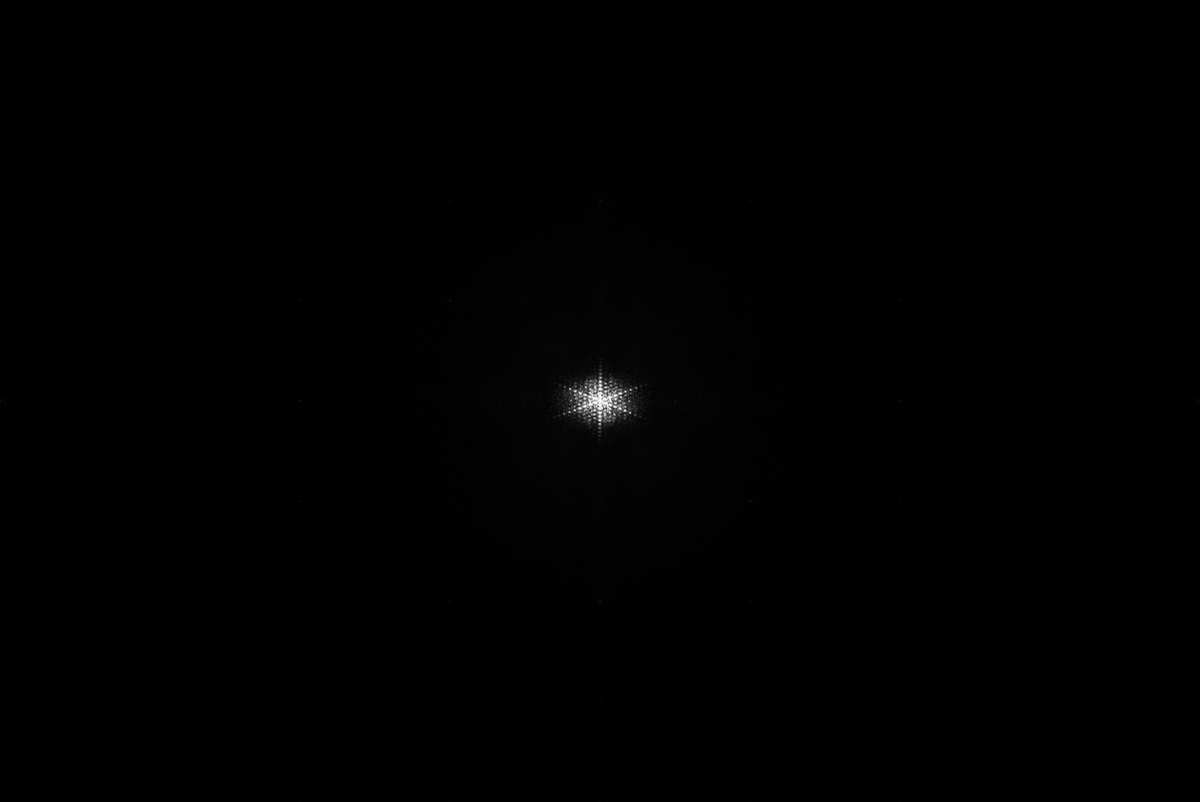
\includegraphics[ width = 0.95 \linewidth ]{figures/CalculatedFT/1547_FT_LinearPlot.png}
        \caption{The calculated FT using the aperture with a diameter of $1.0 \ \si{mm}$}
    \end{minipage}%
    \hspace{0.5cm}
    \begin{minipage}[t]{0.45\textwidth}
        \centering
        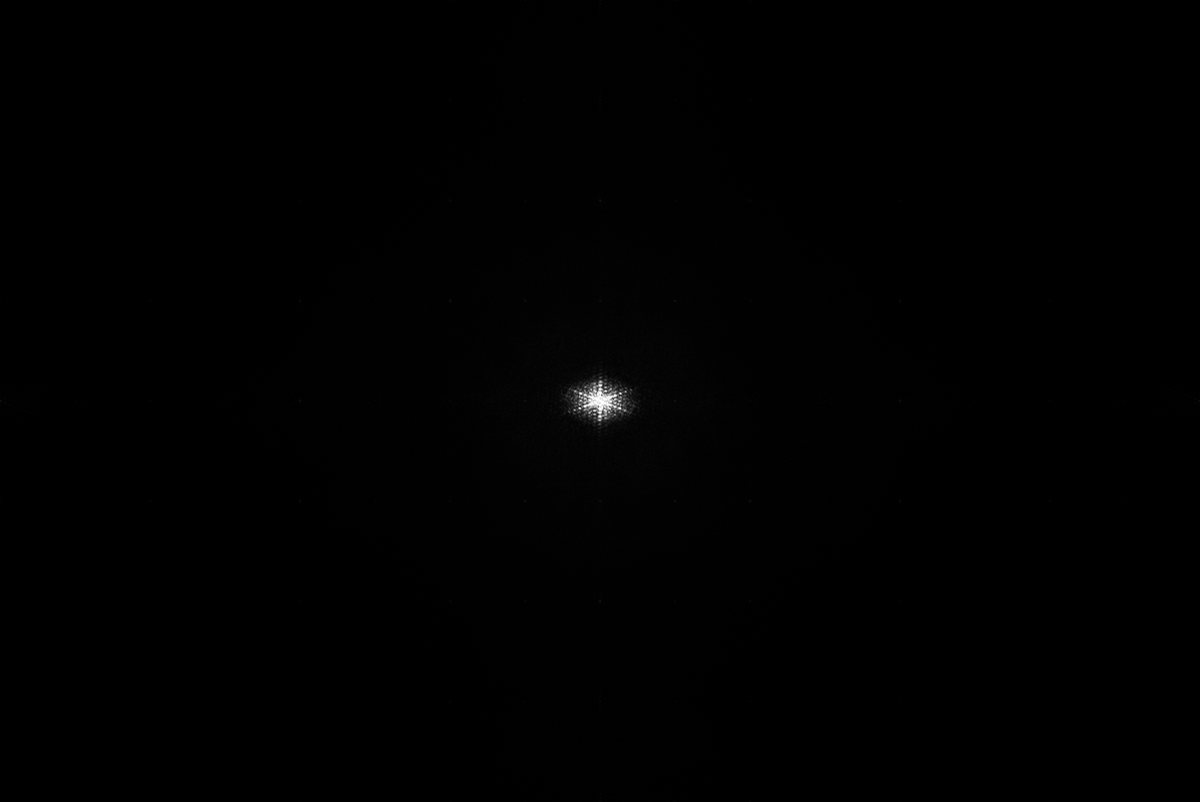
\includegraphics[ width = 0.95 \linewidth ]{figures/CalculatedFT/1546_FT_LinearPlot.png}
        \caption{The calculated FT using the aperture with a diameter of $0.70 \ \si{mm}$}
    \end{minipage}%
    \vspace{1.5cm}
    \begin{minipage}[t]{0.45\textwidth}
        \centering
        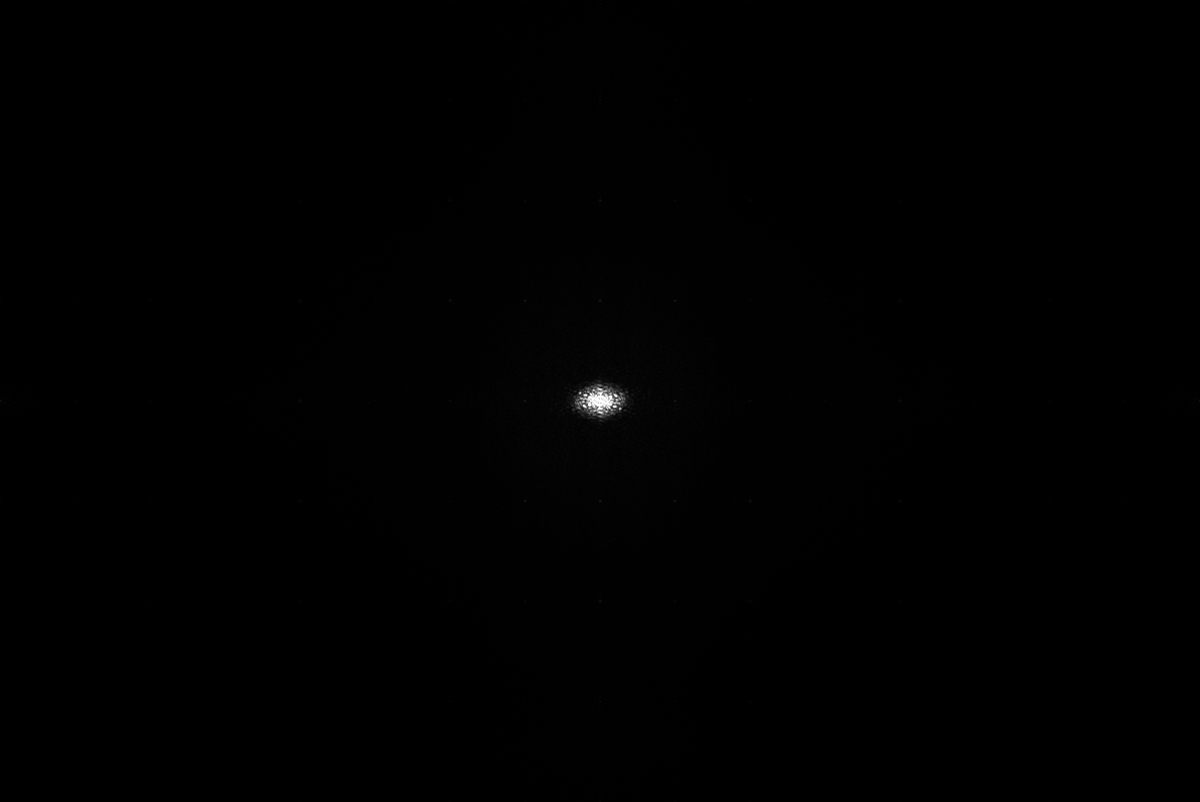
\includegraphics[ width = 0.95 \linewidth ]{figures/CalculatedFT/1545_FT_LinearPlot.png}
        \caption{The calculated FT using the aperture with a diameter of $0.50 \ \si{mm}$}
    \end{minipage}%
    \hspace{0.5cm}
    \begin{minipage}[t]{0.45\textwidth}
        \centering
        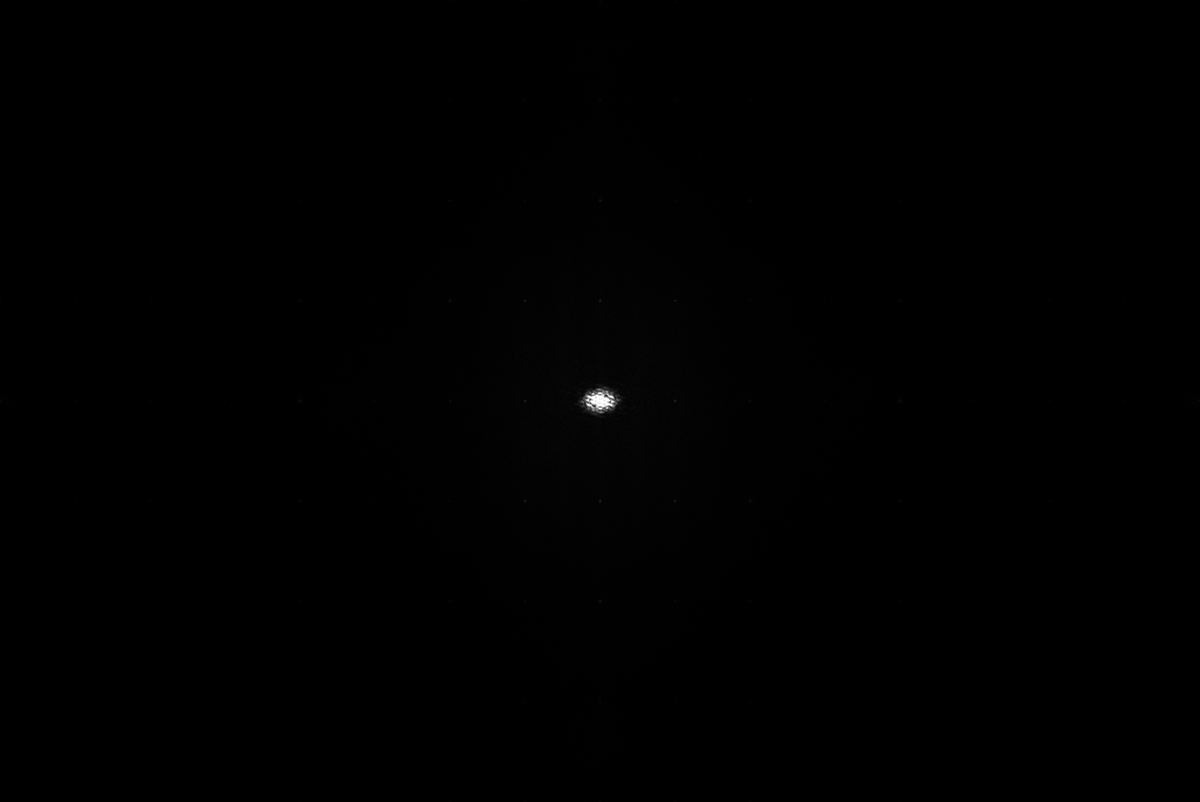
\includegraphics[ width = 0.95 \linewidth ]{figures/CalculatedFT/1544_FT_LinearPlot.png}
        \caption{The calculated FT using the aperture with a diameter of $0.30 \ \si{mm}$}
    \end{minipage}%
\end{figure}

\subsection{Gradient Images}
All the gradient images below correspond to the images we captured in Part E of the appendix.
\begin{figure}[H]
    \centering
    \begin{minipage}{0.45\textwidth}
        \centering
        
\includegraphics[ width = 0.95 \linewidth ]{figures/GradientImages/1549G.jpg}
        \caption{The gradient image of the captured inverse Fourier transform with no aperture}
    \end{minipage}%
    \hspace{0.75cm}
    \begin{minipage}{0.45\textwidth}
        \centering
        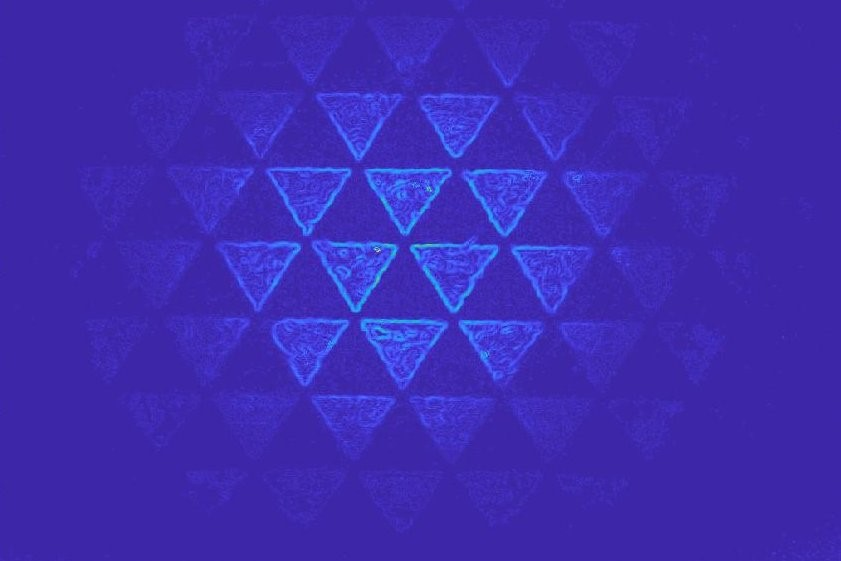
\includegraphics[ width = 0.95 \linewidth ]{figures/GradientImages/1548G.jpg}
        \caption{The gradient image of the captured inverse Fourier transform using the aperture with a diameter of $2.0 \ \si{mm}$}
    \end{minipage}%
    \vspace{1cm}
    \begin{minipage}{0.45\textwidth}
        \centering
        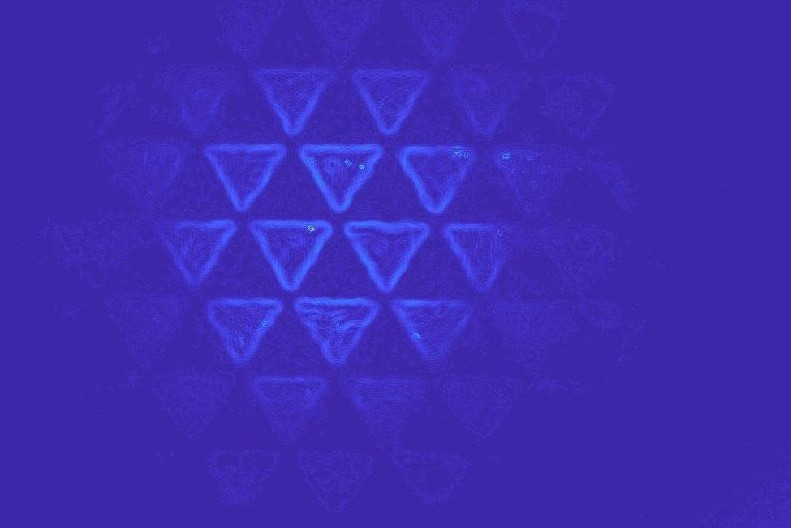
\includegraphics[ width = 0.95 \linewidth ]{figures/GradientImages/1547G.jpg}
        \caption{The gradient image of the captured inverse Fourier transform using the aperture with a diameter of $1.0 \ \si{mm}$}
    \end{minipage}%
    \hspace{0.75cm}
    \begin{minipage}{0.45\textwidth}
        \centering
        \includegraphics[ width = 0.95 \linewidth ]{figures/GradientImages/1546G.png}
        \caption{The gradient image of the captured inverse Fourier transform using the aperture with a diameter of $0.7 \ \si{mm}$}
    \end{minipage}%
    \vspace{1cm}
    \begin{minipage}{0.45\textwidth}
        \centering
        \includegraphics[ width = 0.95 \linewidth ]{figures/GradientImages/1545G.png}
        \caption{The gradient image of the captured inverse Fourier transform using the aperture with a diameter of $0.5 \ \si{mm}$}
    \end{minipage}%
    \hspace{0.75cm}
    \begin{minipage}{0.45\textwidth}
        \centering
        \includegraphics[ width = 0.95 \linewidth ]{figures/GradientImages/1544G.png}
        \caption{The gradient image of the captured inverse Fourier transform using the aperture with a diameter of $0.3 \ \si{mm}$}
    \end{minipage}%
\end{figure}
\end{document}